\documentclass[]{article}
\usepackage{lmodern}
\usepackage{amssymb,amsmath}
\usepackage{ifxetex,ifluatex}
\usepackage{fixltx2e} % provides \textsubscript
\ifnum 0\ifxetex 1\fi\ifluatex 1\fi=0 % if pdftex
  \usepackage[T1]{fontenc}
  \usepackage[utf8]{inputenc}
\else % if luatex or xelatex
  \ifxetex
    \usepackage{mathspec}
  \else
    \usepackage{fontspec}
  \fi
  \defaultfontfeatures{Ligatures=TeX,Scale=MatchLowercase}
\fi
% use upquote if available, for straight quotes in verbatim environments
\IfFileExists{upquote.sty}{\usepackage{upquote}}{}
% use microtype if available
\IfFileExists{microtype.sty}{%
\usepackage{microtype}
\UseMicrotypeSet[protrusion]{basicmath} % disable protrusion for tt fonts
}{}
\usepackage[margin=1in]{geometry}
\usepackage{hyperref}
\hypersetup{unicode=true,
            pdfborder={0 0 0},
            breaklinks=true}
\urlstyle{same}  % don't use monospace font for urls
\usepackage{color}
\usepackage{fancyvrb}
\newcommand{\VerbBar}{|}
\newcommand{\VERB}{\Verb[commandchars=\\\{\}]}
\DefineVerbatimEnvironment{Highlighting}{Verbatim}{commandchars=\\\{\}}
% Add ',fontsize=\small' for more characters per line
\usepackage{framed}
\definecolor{shadecolor}{RGB}{248,248,248}
\newenvironment{Shaded}{\begin{snugshade}}{\end{snugshade}}
\newcommand{\KeywordTok}[1]{\textcolor[rgb]{0.13,0.29,0.53}{\textbf{#1}}}
\newcommand{\DataTypeTok}[1]{\textcolor[rgb]{0.13,0.29,0.53}{#1}}
\newcommand{\DecValTok}[1]{\textcolor[rgb]{0.00,0.00,0.81}{#1}}
\newcommand{\BaseNTok}[1]{\textcolor[rgb]{0.00,0.00,0.81}{#1}}
\newcommand{\FloatTok}[1]{\textcolor[rgb]{0.00,0.00,0.81}{#1}}
\newcommand{\ConstantTok}[1]{\textcolor[rgb]{0.00,0.00,0.00}{#1}}
\newcommand{\CharTok}[1]{\textcolor[rgb]{0.31,0.60,0.02}{#1}}
\newcommand{\SpecialCharTok}[1]{\textcolor[rgb]{0.00,0.00,0.00}{#1}}
\newcommand{\StringTok}[1]{\textcolor[rgb]{0.31,0.60,0.02}{#1}}
\newcommand{\VerbatimStringTok}[1]{\textcolor[rgb]{0.31,0.60,0.02}{#1}}
\newcommand{\SpecialStringTok}[1]{\textcolor[rgb]{0.31,0.60,0.02}{#1}}
\newcommand{\ImportTok}[1]{#1}
\newcommand{\CommentTok}[1]{\textcolor[rgb]{0.56,0.35,0.01}{\textit{#1}}}
\newcommand{\DocumentationTok}[1]{\textcolor[rgb]{0.56,0.35,0.01}{\textbf{\textit{#1}}}}
\newcommand{\AnnotationTok}[1]{\textcolor[rgb]{0.56,0.35,0.01}{\textbf{\textit{#1}}}}
\newcommand{\CommentVarTok}[1]{\textcolor[rgb]{0.56,0.35,0.01}{\textbf{\textit{#1}}}}
\newcommand{\OtherTok}[1]{\textcolor[rgb]{0.56,0.35,0.01}{#1}}
\newcommand{\FunctionTok}[1]{\textcolor[rgb]{0.00,0.00,0.00}{#1}}
\newcommand{\VariableTok}[1]{\textcolor[rgb]{0.00,0.00,0.00}{#1}}
\newcommand{\ControlFlowTok}[1]{\textcolor[rgb]{0.13,0.29,0.53}{\textbf{#1}}}
\newcommand{\OperatorTok}[1]{\textcolor[rgb]{0.81,0.36,0.00}{\textbf{#1}}}
\newcommand{\BuiltInTok}[1]{#1}
\newcommand{\ExtensionTok}[1]{#1}
\newcommand{\PreprocessorTok}[1]{\textcolor[rgb]{0.56,0.35,0.01}{\textit{#1}}}
\newcommand{\AttributeTok}[1]{\textcolor[rgb]{0.77,0.63,0.00}{#1}}
\newcommand{\RegionMarkerTok}[1]{#1}
\newcommand{\InformationTok}[1]{\textcolor[rgb]{0.56,0.35,0.01}{\textbf{\textit{#1}}}}
\newcommand{\WarningTok}[1]{\textcolor[rgb]{0.56,0.35,0.01}{\textbf{\textit{#1}}}}
\newcommand{\AlertTok}[1]{\textcolor[rgb]{0.94,0.16,0.16}{#1}}
\newcommand{\ErrorTok}[1]{\textcolor[rgb]{0.64,0.00,0.00}{\textbf{#1}}}
\newcommand{\NormalTok}[1]{#1}
\usepackage{graphicx,grffile}
\makeatletter
\def\maxwidth{\ifdim\Gin@nat@width>\linewidth\linewidth\else\Gin@nat@width\fi}
\def\maxheight{\ifdim\Gin@nat@height>\textheight\textheight\else\Gin@nat@height\fi}
\makeatother
% Scale images if necessary, so that they will not overflow the page
% margins by default, and it is still possible to overwrite the defaults
% using explicit options in \includegraphics[width, height, ...]{}
\setkeys{Gin}{width=\maxwidth,height=\maxheight,keepaspectratio}
\IfFileExists{parskip.sty}{%
\usepackage{parskip}
}{% else
\setlength{\parindent}{0pt}
\setlength{\parskip}{6pt plus 2pt minus 1pt}
}
\setlength{\emergencystretch}{3em}  % prevent overfull lines
\providecommand{\tightlist}{%
  \setlength{\itemsep}{0pt}\setlength{\parskip}{0pt}}
\setcounter{secnumdepth}{0}
% Redefines (sub)paragraphs to behave more like sections
\ifx\paragraph\undefined\else
\let\oldparagraph\paragraph
\renewcommand{\paragraph}[1]{\oldparagraph{#1}\mbox{}}
\fi
\ifx\subparagraph\undefined\else
\let\oldsubparagraph\subparagraph
\renewcommand{\subparagraph}[1]{\oldsubparagraph{#1}\mbox{}}
\fi

%%% Use protect on footnotes to avoid problems with footnotes in titles
\let\rmarkdownfootnote\footnote%
\def\footnote{\protect\rmarkdownfootnote}

%%% Change title format to be more compact
\usepackage{titling}

% Create subtitle command for use in maketitle
\newcommand{\subtitle}[1]{
  \posttitle{
    \begin{center}\large#1\end{center}
    }
}

\setlength{\droptitle}{-2em}
  \title{}
  \pretitle{\vspace{\droptitle}}
  \posttitle{}
  \author{}
  \preauthor{}\postauthor{}
  \date{}
  \predate{}\postdate{}


\begin{document}

\section{White Wine Quality Analysis - Divya
Chandramouli}\label{white-wine-quality-analysis---divya-chandramouli}

Load the data and print the names of variables in the dataset

\begin{verbatim}
##  [1] "X"                    "fixed.acidity"        "volatile.acidity"    
##  [4] "citric.acid"          "residual.sugar"       "chlorides"           
##  [7] "free.sulfur.dioxide"  "total.sulfur.dioxide" "density"             
## [10] "pH"                   "sulphates"            "alcohol"             
## [13] "quality"
\end{verbatim}

\subsection{Introduction to the
dataset}\label{introduction-to-the-dataset}

This dataset contains data on white variants of the Portuguese ``Vinho
Verde'' wine. There are 11 variables quantifying the chemical properties
of each wine. At least 3 wine experts rated the quality of each wine,
providing a rating between 0 (very bad) and 10 (very excellent).This
dataset is publicly available for research.

Citation: P. Cortez, A. Cerdeira, F. Almeida, T. Matos and J. Reis.
Modeling wine preferences by data mining from physicochemical
properties. In Decision Support Systems, Elsevier, 47(4):547-553. ISSN:
0167-9236.

The inputs include objective tests (e.g.~PH values) and the output is
based on sensory data (median of at least 3 evaluations made by wine
experts).

\subsection{Description of Attributes}\label{description-of-attributes}

\begin{enumerate}
\def\labelenumi{\arabic{enumi}.}
\item
  Fixed acidity: most acids involved with wine or fixed or nonvolatile
  (do not evaporate readily)
\item
  Volatile acidity: the amount of acetic acid in wine, which at too high
  of levels can lead to an unpleasant, vinegar taste
\item
  Citric acid: found in small quantities, citric acid can add
  `freshness' and flavor to wines
\item
  Residual sugar: the amount of sugar remaining after fermentation
  stops, it's rare to find wines with less than 1 gram/liter and wines
  with greater than 45 grams/liter are considered sweet
\item
  Chlorides: the amount of salt in the wine
\item
  Free sulfur dioxide: the free form of SO2 exists in equilibrium
  between molecular SO2 (as a dissolved gas) and bisulfite ion; it
  prevents microbial growth and the oxidation of wine
\item
  Total sulfur dioxide: amount of free and bound forms of S02; in low
  concentrations, SO2 is mostly undetectable in wine, but at free SO2
  concentrations over 50 ppm, SO2 becomes evident in the nose and taste
  of wine
\item
  Density: the density of water is close to that of water depending on
  the percent alcohol and sugar content
\item
  pH: describes how acidic or basic a wine is on a scale from 0 (very
  acidic) to 14 (very basic); most wines are between 3-4 on the pH scale
\item
  Sulphates: a wine additive which can contribute to sulfur dioxide gas
  (S02) levels, wich acts as an antimicrobial and antioxidant
\item
  Alcohol: the percent alcohol content of the wine

  Output variable (based on sensory data):
\item
  Quality (score between 0 and 10)
\end{enumerate}

\subsection{Research Question}\label{research-question}

This project investigates which chemical properties influence the
quality of white wines

\subsection{Understanding the dataset}\label{understanding-the-dataset}

In this section, we will perform some preliminary exploration of the
dataset- Running some summaries of the data and creating univariate
plots to understand the structure of the individual variables in the
dataset.

\subsubsection{Dimensions of the
dataset}\label{dimensions-of-the-dataset}

\begin{verbatim}
## [1] 4898   13
\end{verbatim}

We have 4898 rows and 13 variables in the dataset - 11 physicochemical
properties, 1 quality rating and 1 index/serial number

\subsubsection{Let's examine the structure of the dataframe, the
variables and the type
of}\label{lets-examine-the-structure-of-the-dataframe-the-variables-and-the-type-of}

data they hold

\begin{verbatim}
## 'data.frame':    4898 obs. of  13 variables:
##  $ X                   : int  1 2 3 4 5 6 7 8 9 10 ...
##  $ fixed.acidity       : num  7 6.3 8.1 7.2 7.2 8.1 6.2 7 6.3 8.1 ...
##  $ volatile.acidity    : num  0.27 0.3 0.28 0.23 0.23 0.28 0.32 0.27 0.3 0.22 ...
##  $ citric.acid         : num  0.36 0.34 0.4 0.32 0.32 0.4 0.16 0.36 0.34 0.43 ...
##  $ residual.sugar      : num  20.7 1.6 6.9 8.5 8.5 6.9 7 20.7 1.6 1.5 ...
##  $ chlorides           : num  0.045 0.049 0.05 0.058 0.058 0.05 0.045 0.045 0.049 0.044 ...
##  $ free.sulfur.dioxide : num  45 14 30 47 47 30 30 45 14 28 ...
##  $ total.sulfur.dioxide: num  170 132 97 186 186 97 136 170 132 129 ...
##  $ density             : num  1.001 0.994 0.995 0.996 0.996 ...
##  $ pH                  : num  3 3.3 3.26 3.19 3.19 3.26 3.18 3 3.3 3.22 ...
##  $ sulphates           : num  0.45 0.49 0.44 0.4 0.4 0.44 0.47 0.45 0.49 0.45 ...
##  $ alcohol             : num  8.8 9.5 10.1 9.9 9.9 10.1 9.6 8.8 9.5 11 ...
##  $ quality             : int  6 6 6 6 6 6 6 6 6 6 ...
\end{verbatim}

\subsubsection{Summary of the dataset}\label{summary-of-the-dataset}

\begin{verbatim}
##        X        fixed.acidity    volatile.acidity  citric.acid    
##  Min.   :   1   Min.   : 3.800   Min.   :0.0800   Min.   :0.0000  
##  1st Qu.:1225   1st Qu.: 6.300   1st Qu.:0.2100   1st Qu.:0.2700  
##  Median :2450   Median : 6.800   Median :0.2600   Median :0.3200  
##  Mean   :2450   Mean   : 6.855   Mean   :0.2782   Mean   :0.3342  
##  3rd Qu.:3674   3rd Qu.: 7.300   3rd Qu.:0.3200   3rd Qu.:0.3900  
##  Max.   :4898   Max.   :14.200   Max.   :1.1000   Max.   :1.6600  
##  residual.sugar     chlorides       free.sulfur.dioxide
##  Min.   : 0.600   Min.   :0.00900   Min.   :  2.00     
##  1st Qu.: 1.700   1st Qu.:0.03600   1st Qu.: 23.00     
##  Median : 5.200   Median :0.04300   Median : 34.00     
##  Mean   : 6.391   Mean   :0.04577   Mean   : 35.31     
##  3rd Qu.: 9.900   3rd Qu.:0.05000   3rd Qu.: 46.00     
##  Max.   :65.800   Max.   :0.34600   Max.   :289.00     
##  total.sulfur.dioxide    density             pH          sulphates     
##  Min.   :  9.0        Min.   :0.9871   Min.   :2.720   Min.   :0.2200  
##  1st Qu.:108.0        1st Qu.:0.9917   1st Qu.:3.090   1st Qu.:0.4100  
##  Median :134.0        Median :0.9937   Median :3.180   Median :0.4700  
##  Mean   :138.4        Mean   :0.9940   Mean   :3.188   Mean   :0.4898  
##  3rd Qu.:167.0        3rd Qu.:0.9961   3rd Qu.:3.280   3rd Qu.:0.5500  
##  Max.   :440.0        Max.   :1.0390   Max.   :3.820   Max.   :1.0800  
##     alcohol         quality     
##  Min.   : 8.00   Min.   :3.000  
##  1st Qu.: 9.50   1st Qu.:5.000  
##  Median :10.40   Median :6.000  
##  Mean   :10.51   Mean   :5.878  
##  3rd Qu.:11.40   3rd Qu.:6.000  
##  Max.   :14.20   Max.   :9.000
\end{verbatim}

\subsubsection{Check for missing or null values in the
dataset}\label{check-for-missing-or-null-values-in-the-dataset}

\begin{verbatim}
## [1] FALSE
\end{verbatim}

We do not any have missing values in the dataset

\subsubsection{Are there duplicate records in the
dataset?}\label{are-there-duplicate-records-in-the-dataset}

\begin{verbatim}
## [1] 0
\end{verbatim}

No, the dataset does not have duplicate records

\subsubsection{Univariate exploration}\label{univariate-exploration}

\paragraph{Fixed acidity}\label{fixed-acidity}

\includegraphics{White_wine_quality_files/figure-latex/unnamed-chunk-5-1.pdf}

The distribution of fixed acidity looks like the bell curve and appears
to be normally distributed. The range of fixed acidity is from 3.8 to
14.2 from the summary table. In the plot we can clearly see that the
fixed acidity values for the bulk of wines lies between 4 and 10 with
outliers on the right. 6.8 is the most commonly occurring value of fixed
acidity

\paragraph{Volatile acidity}\label{volatile-acidity}

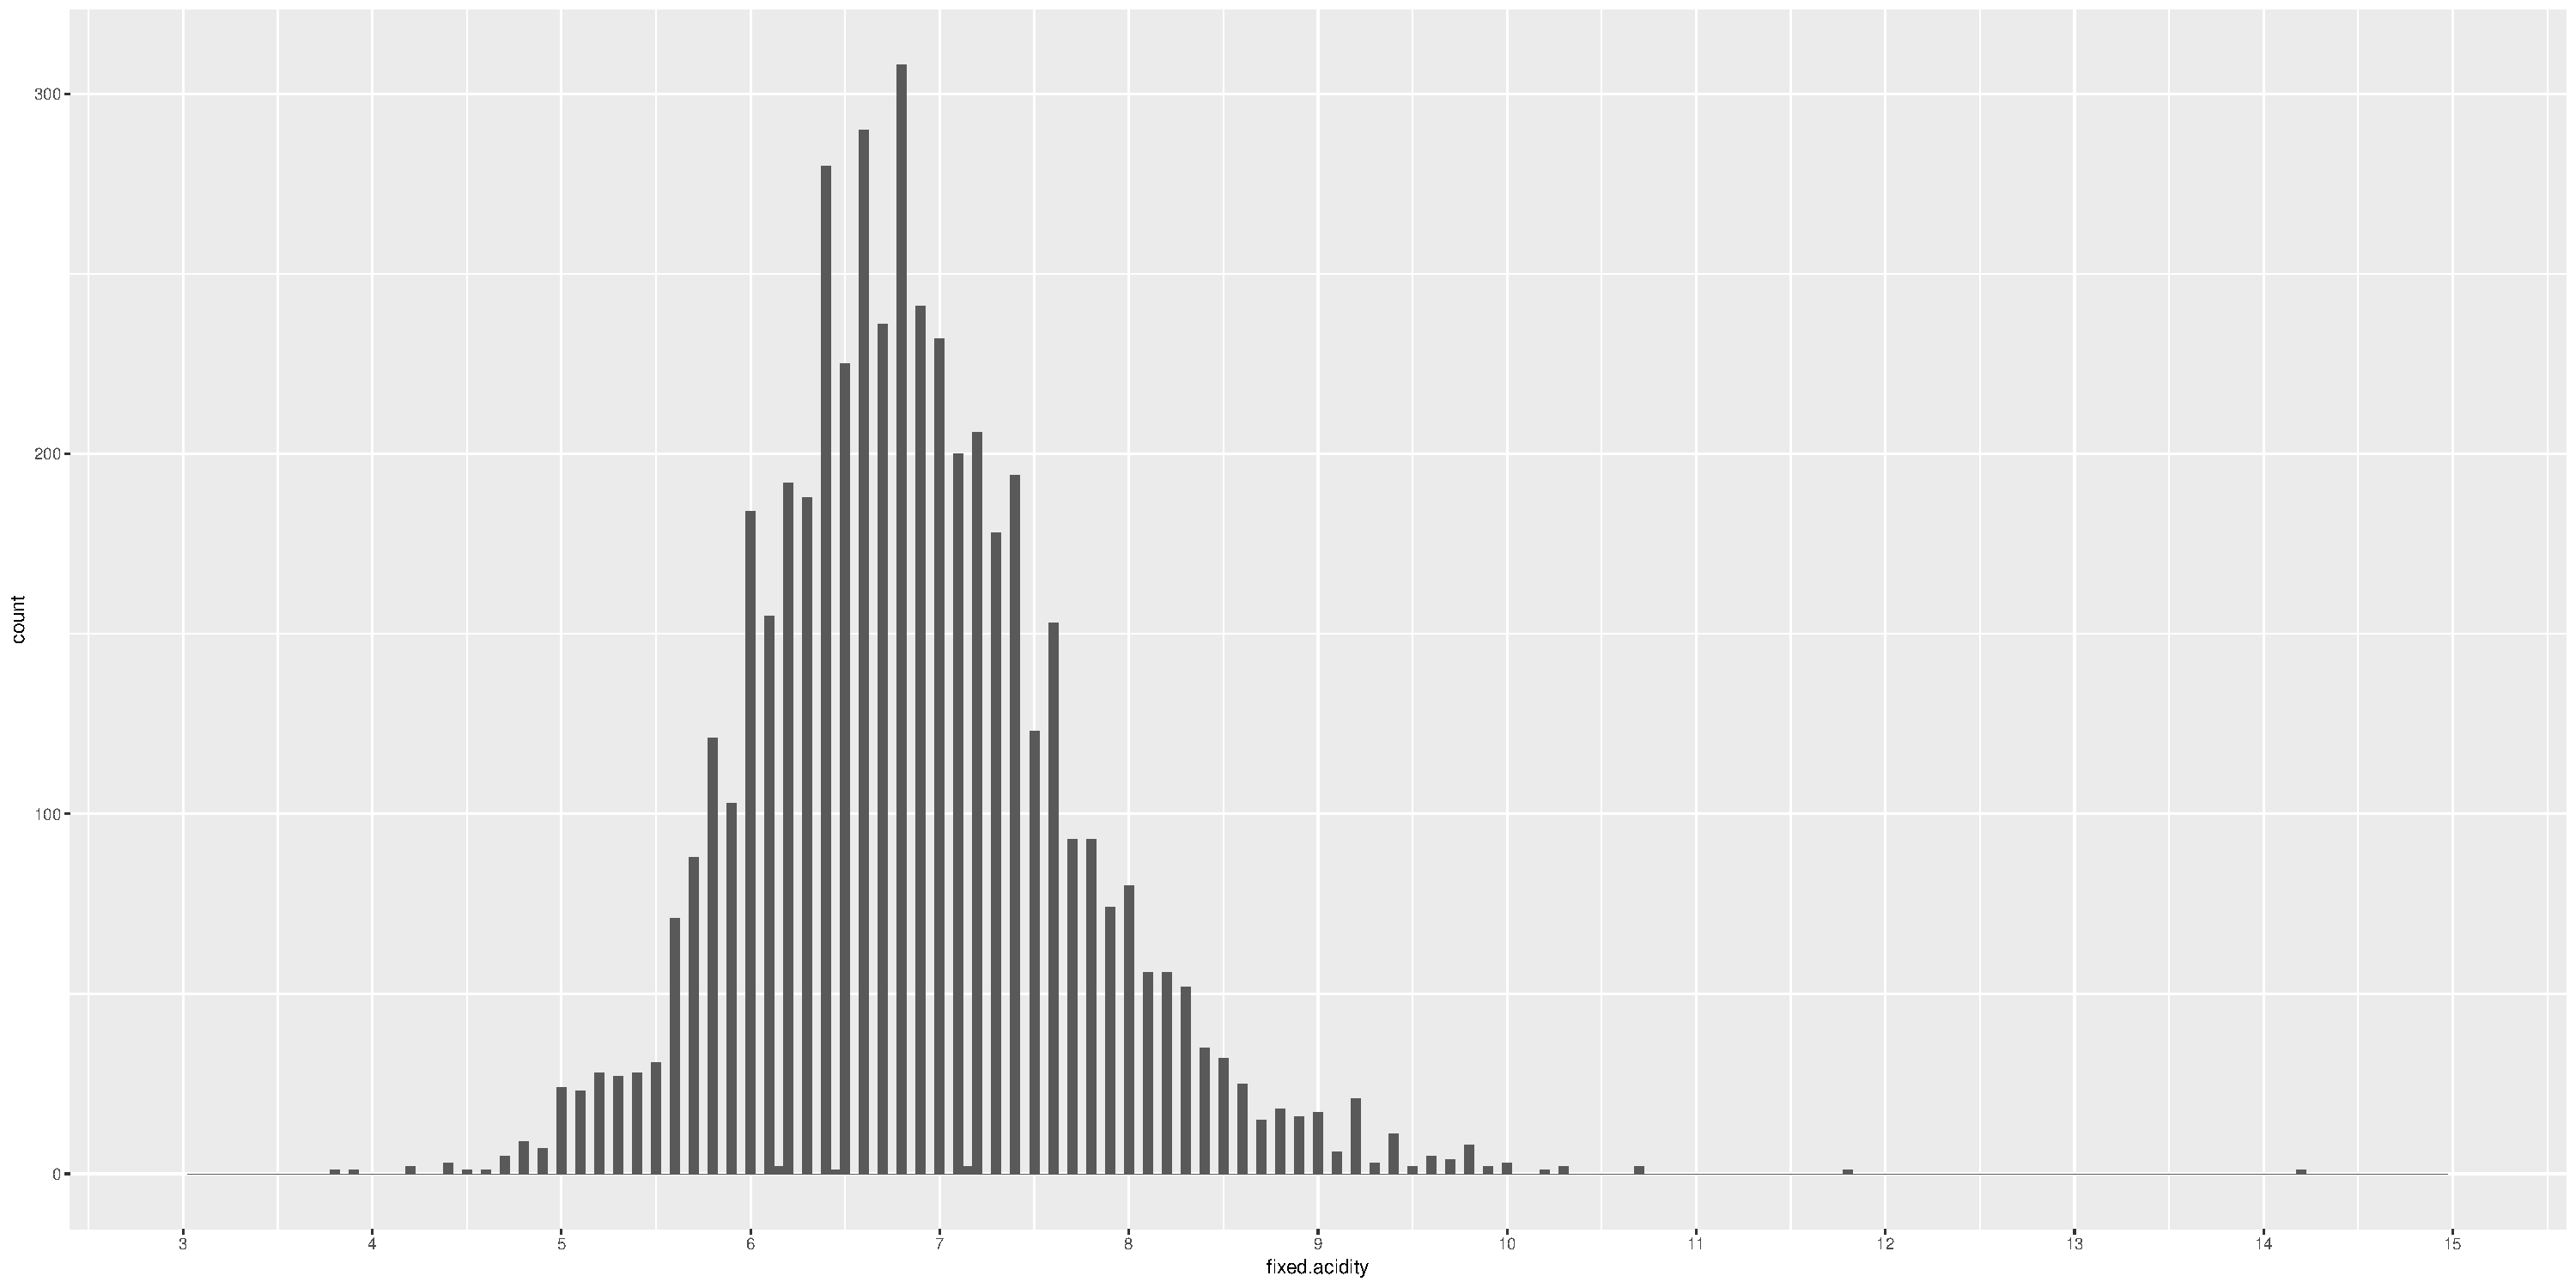
\includegraphics{White_wine_quality_files/figure-latex/unnamed-chunk-6-1.pdf}

The distribution of volatile acidity looks skewed to the right. Most
common value of volatile acidity is 0.28. Bulk of the wines have
volatile acidity value under 0.6.

Since the distribution is skewed to the right, let us try a log10
transform

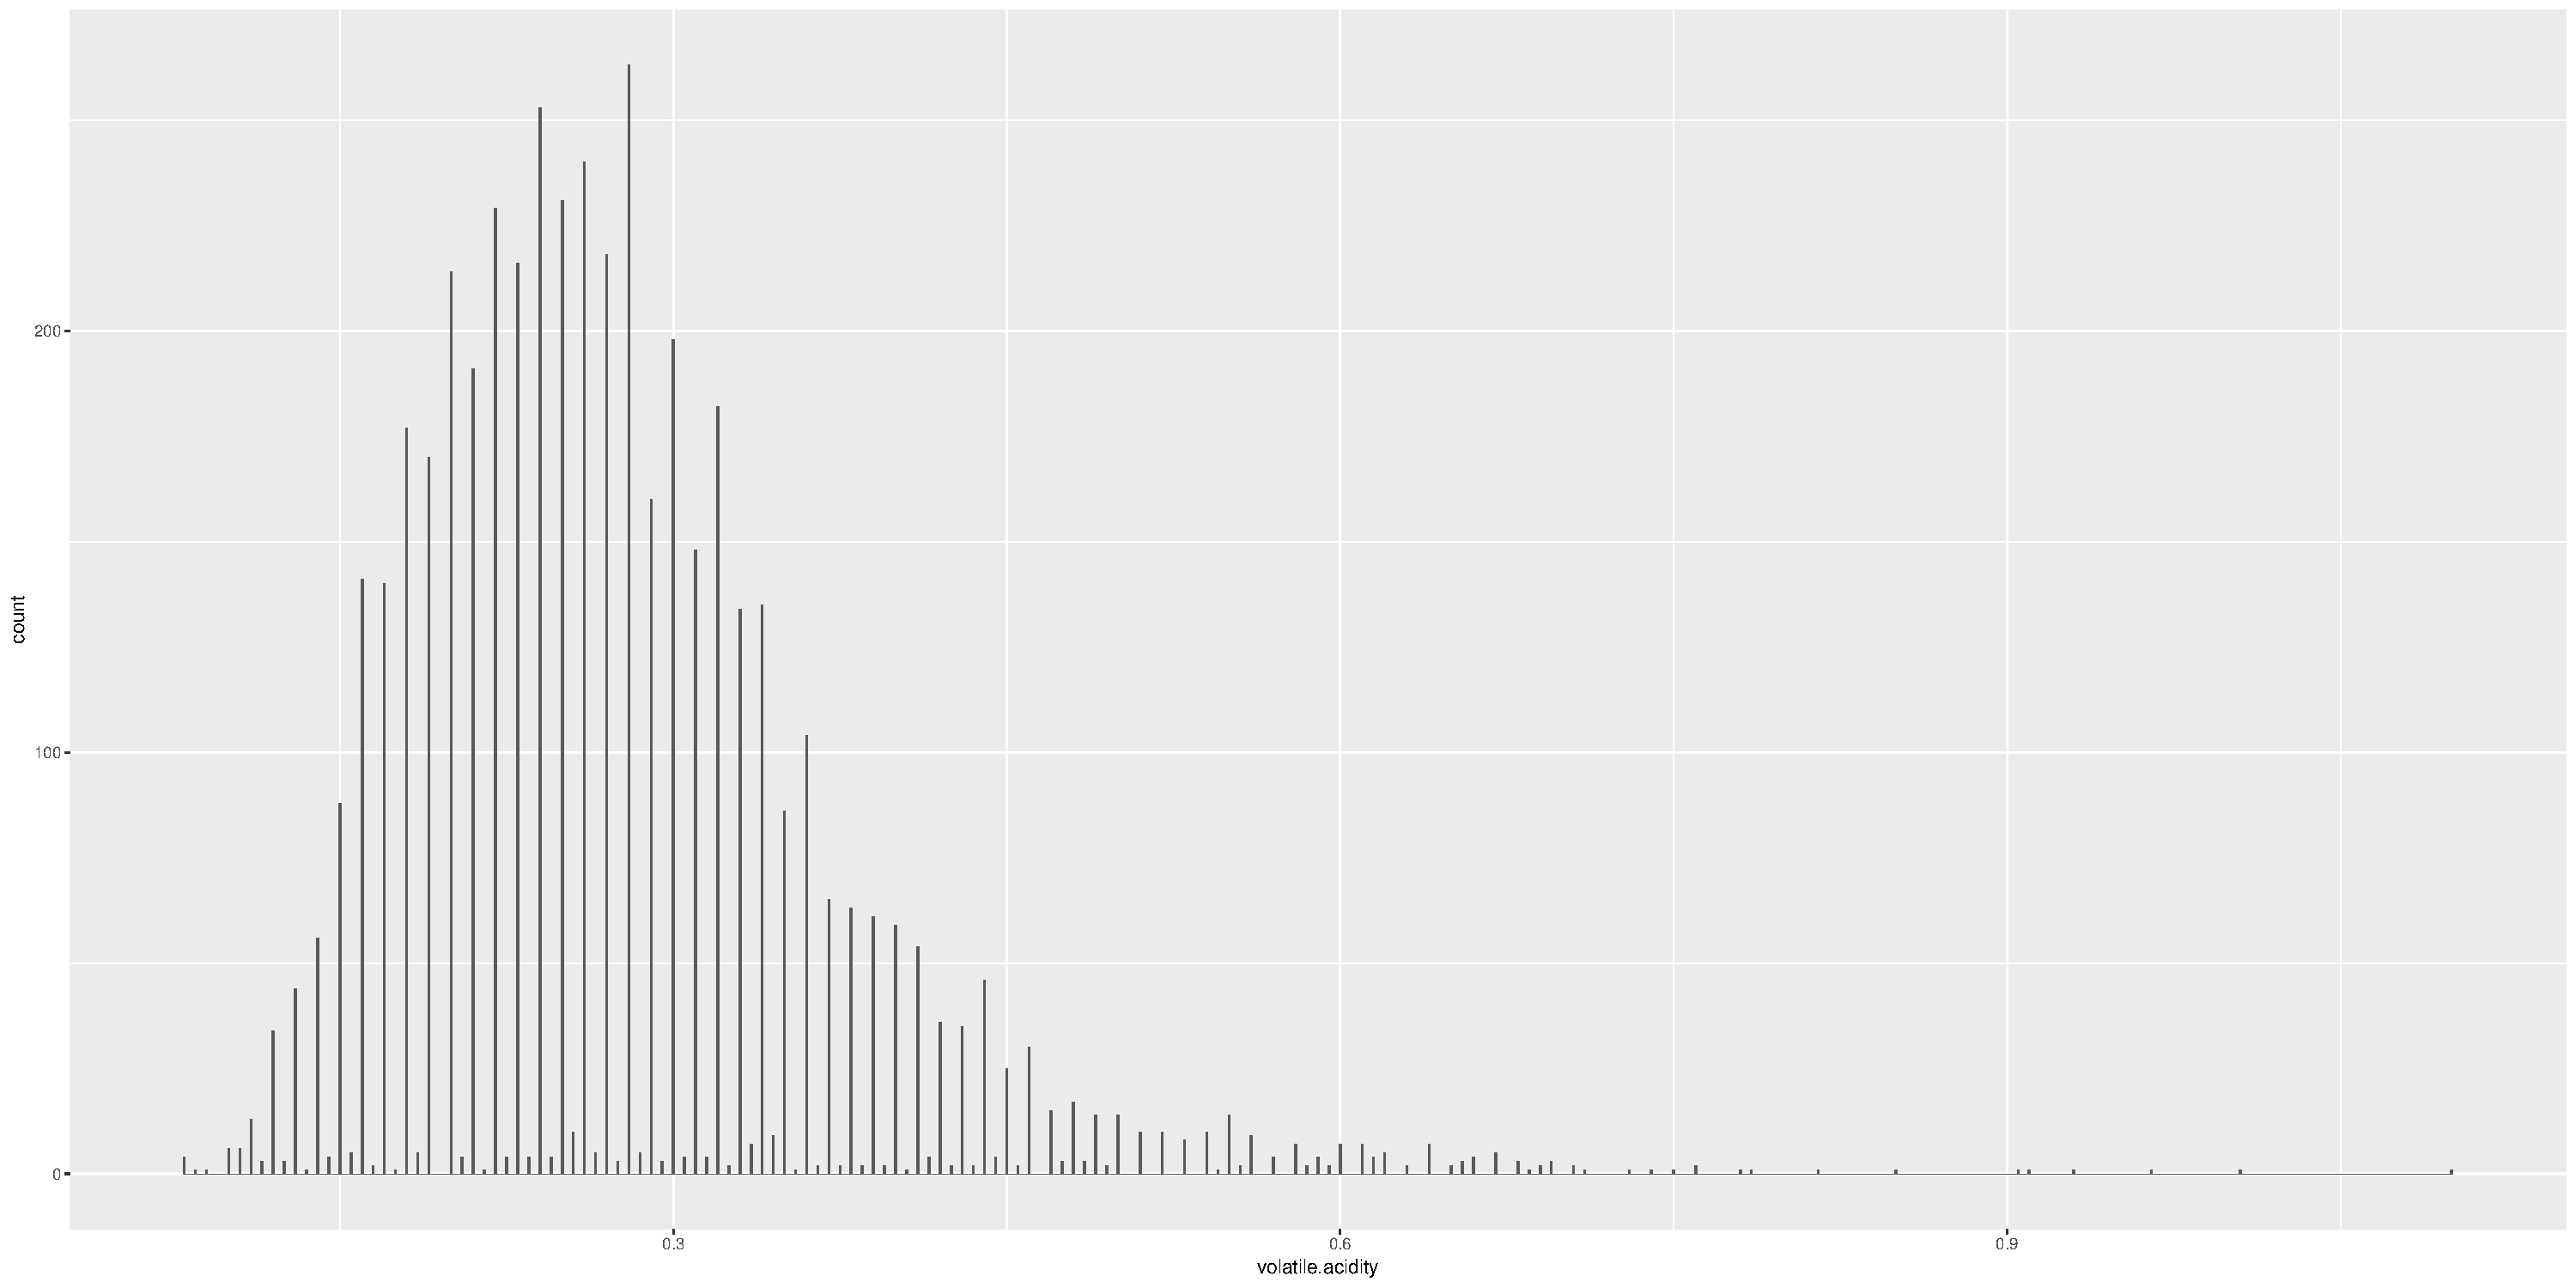
\includegraphics{White_wine_quality_files/figure-latex/unnamed-chunk-7-1.pdf}

Now the distribution looks closer to the bell curve of normal
distribution

\paragraph{Citric acid}\label{citric-acid}

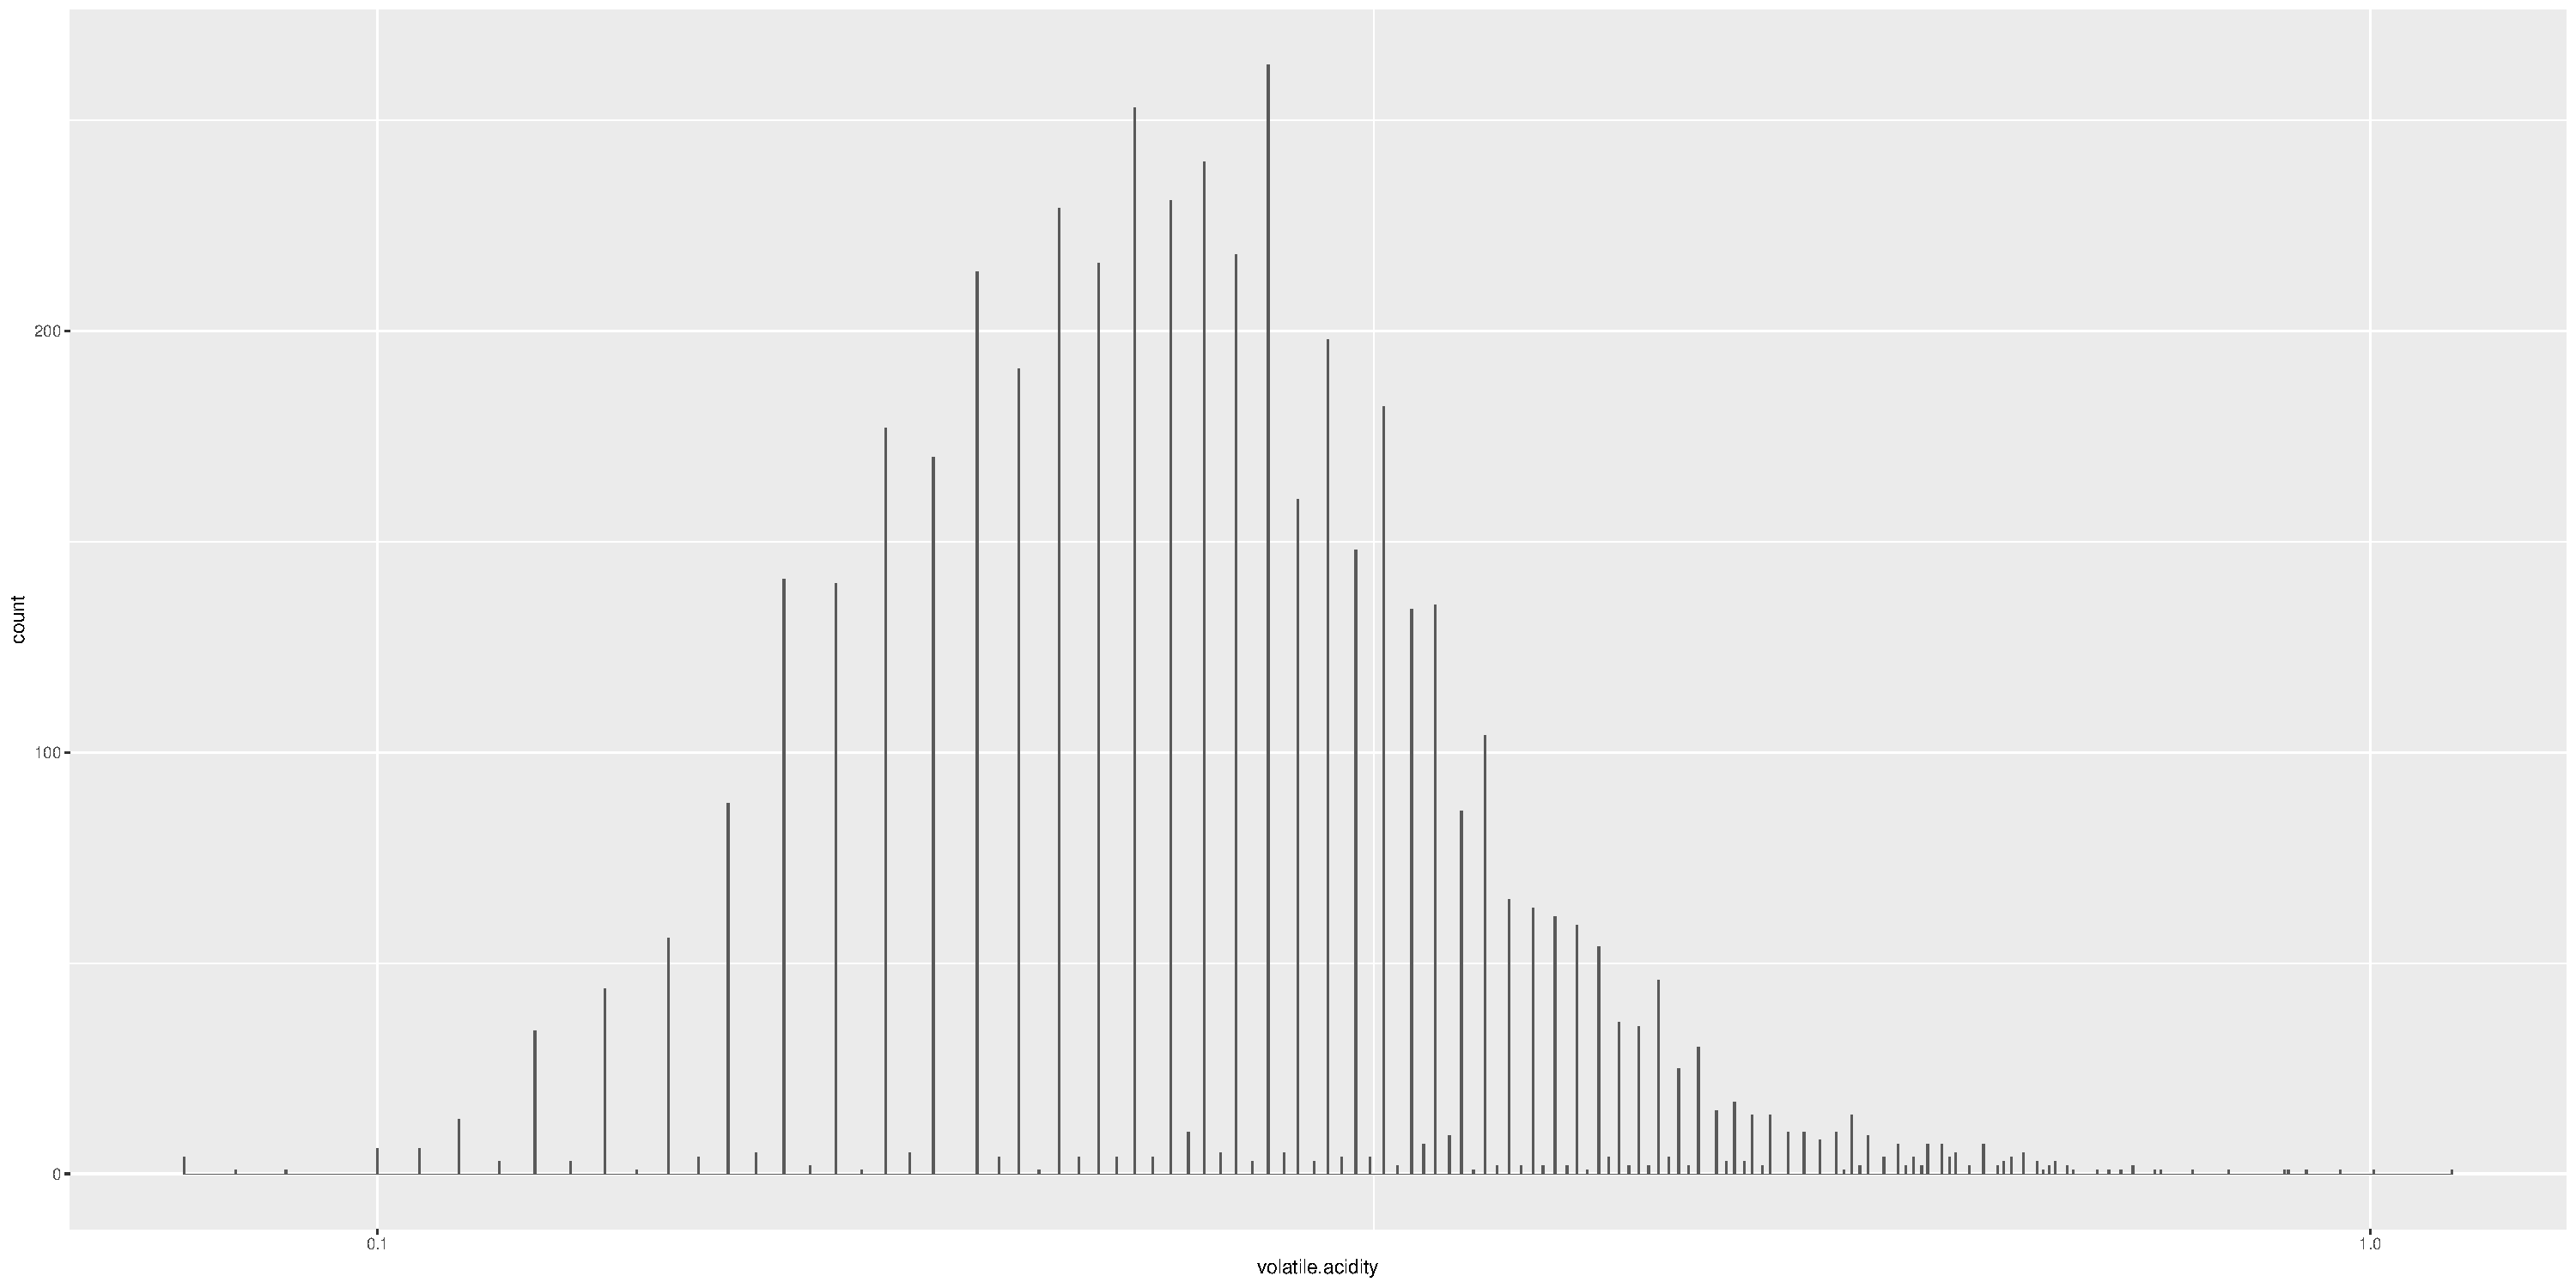
\includegraphics{White_wine_quality_files/figure-latex/unnamed-chunk-8-1.pdf}

Bulk of the citric acid data looks normally distributed. There is an
outlier with the value 1.66

\paragraph{Residual sugar}\label{residual-sugar}

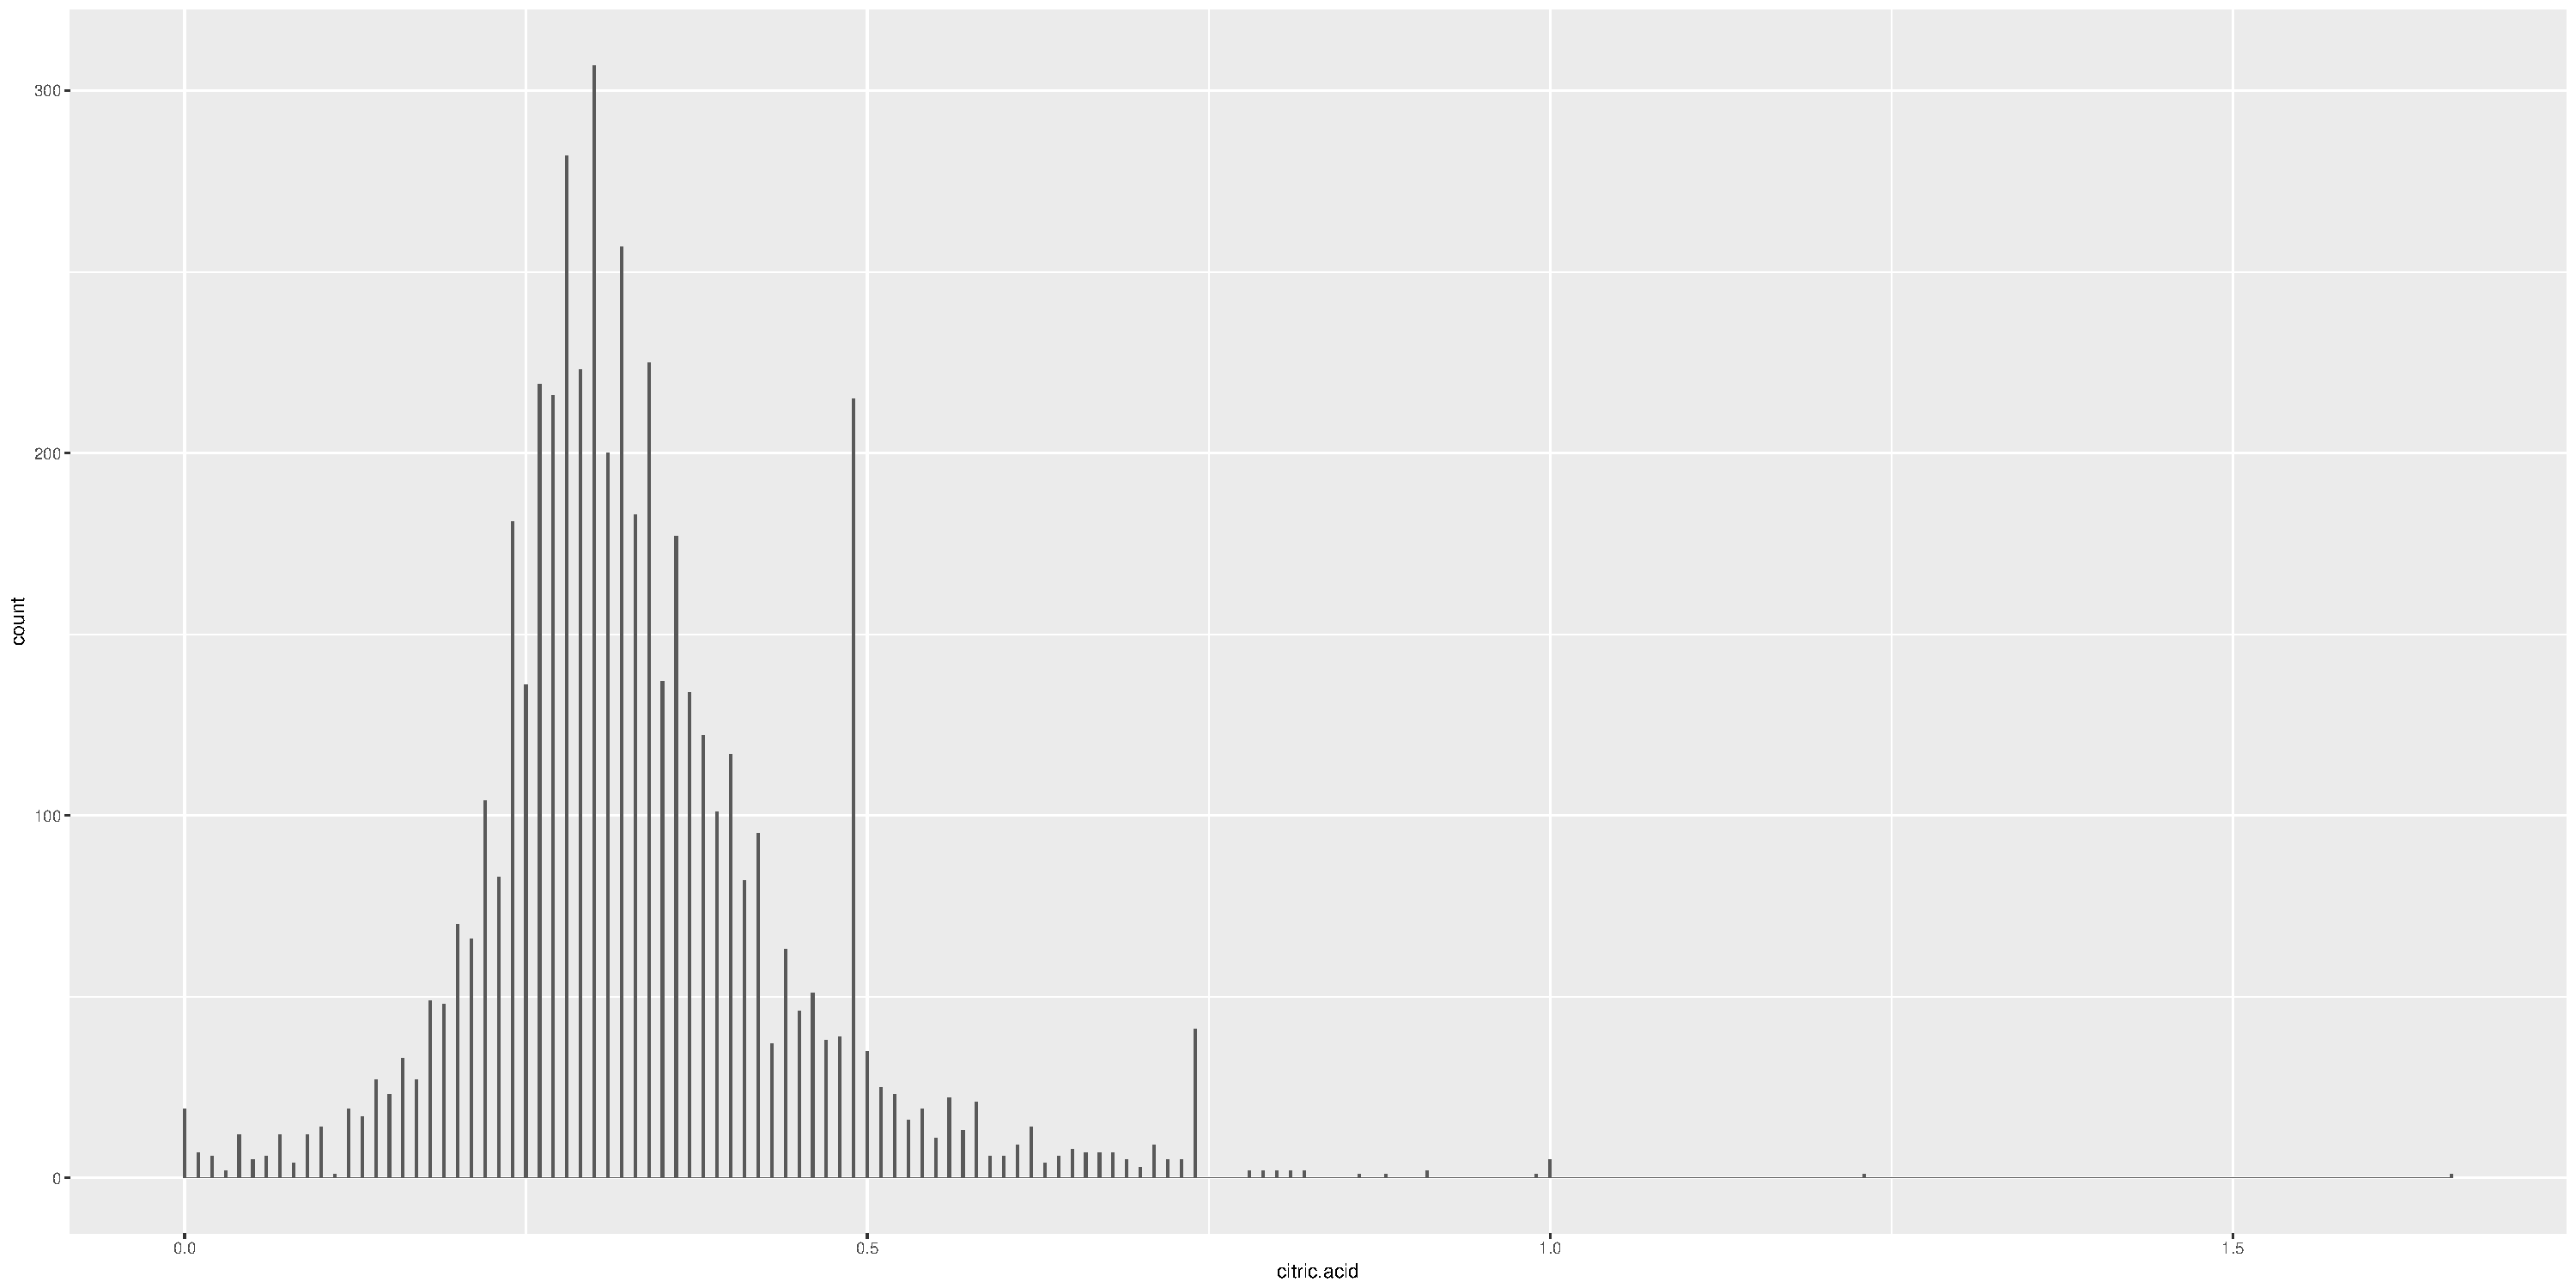
\includegraphics{White_wine_quality_files/figure-latex/unnamed-chunk-9-1.pdf}

The distribution of residual sugar looks clearly skewed to the right
with the maxvalue of 65.8 being an outlier

Let's try a log10 transform on the data

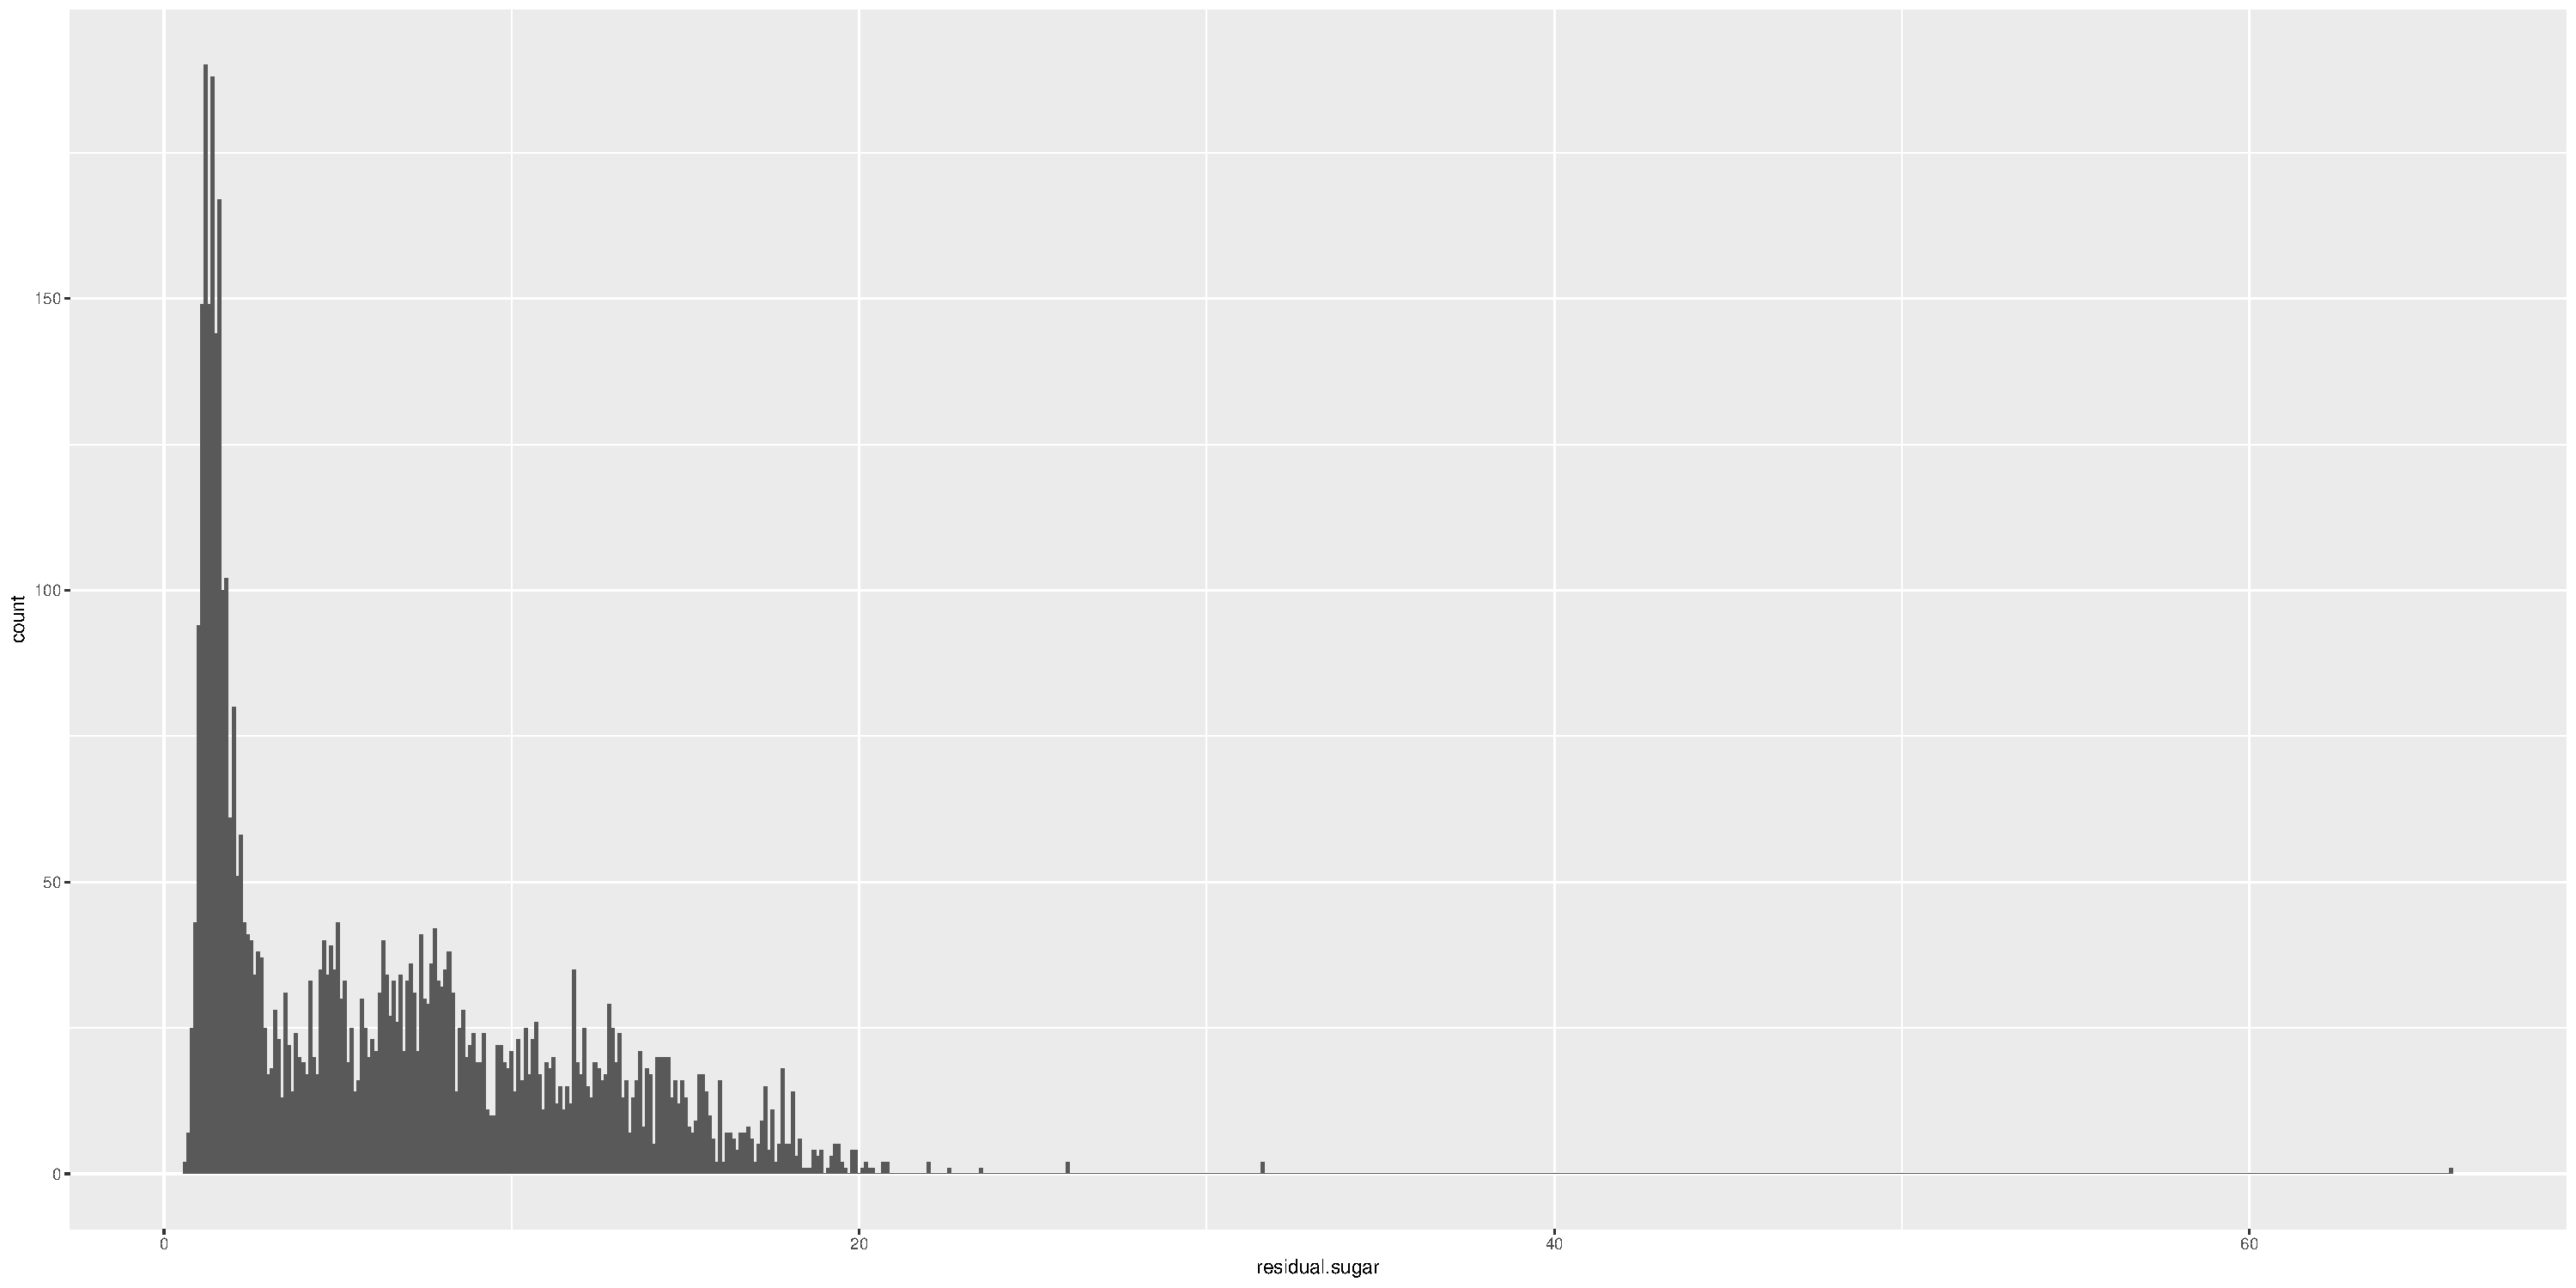
\includegraphics{White_wine_quality_files/figure-latex/unnamed-chunk-10-1.pdf}

Now the distribution looks bimodal with peaks at about 1 and 9 values of
residual sugar

If we trim the top 1\% of residual sugar data, let's see how the
distribution looks

\begin{verbatim}
## Warning: Removed 47 rows containing non-finite values (stat_bin).
\end{verbatim}

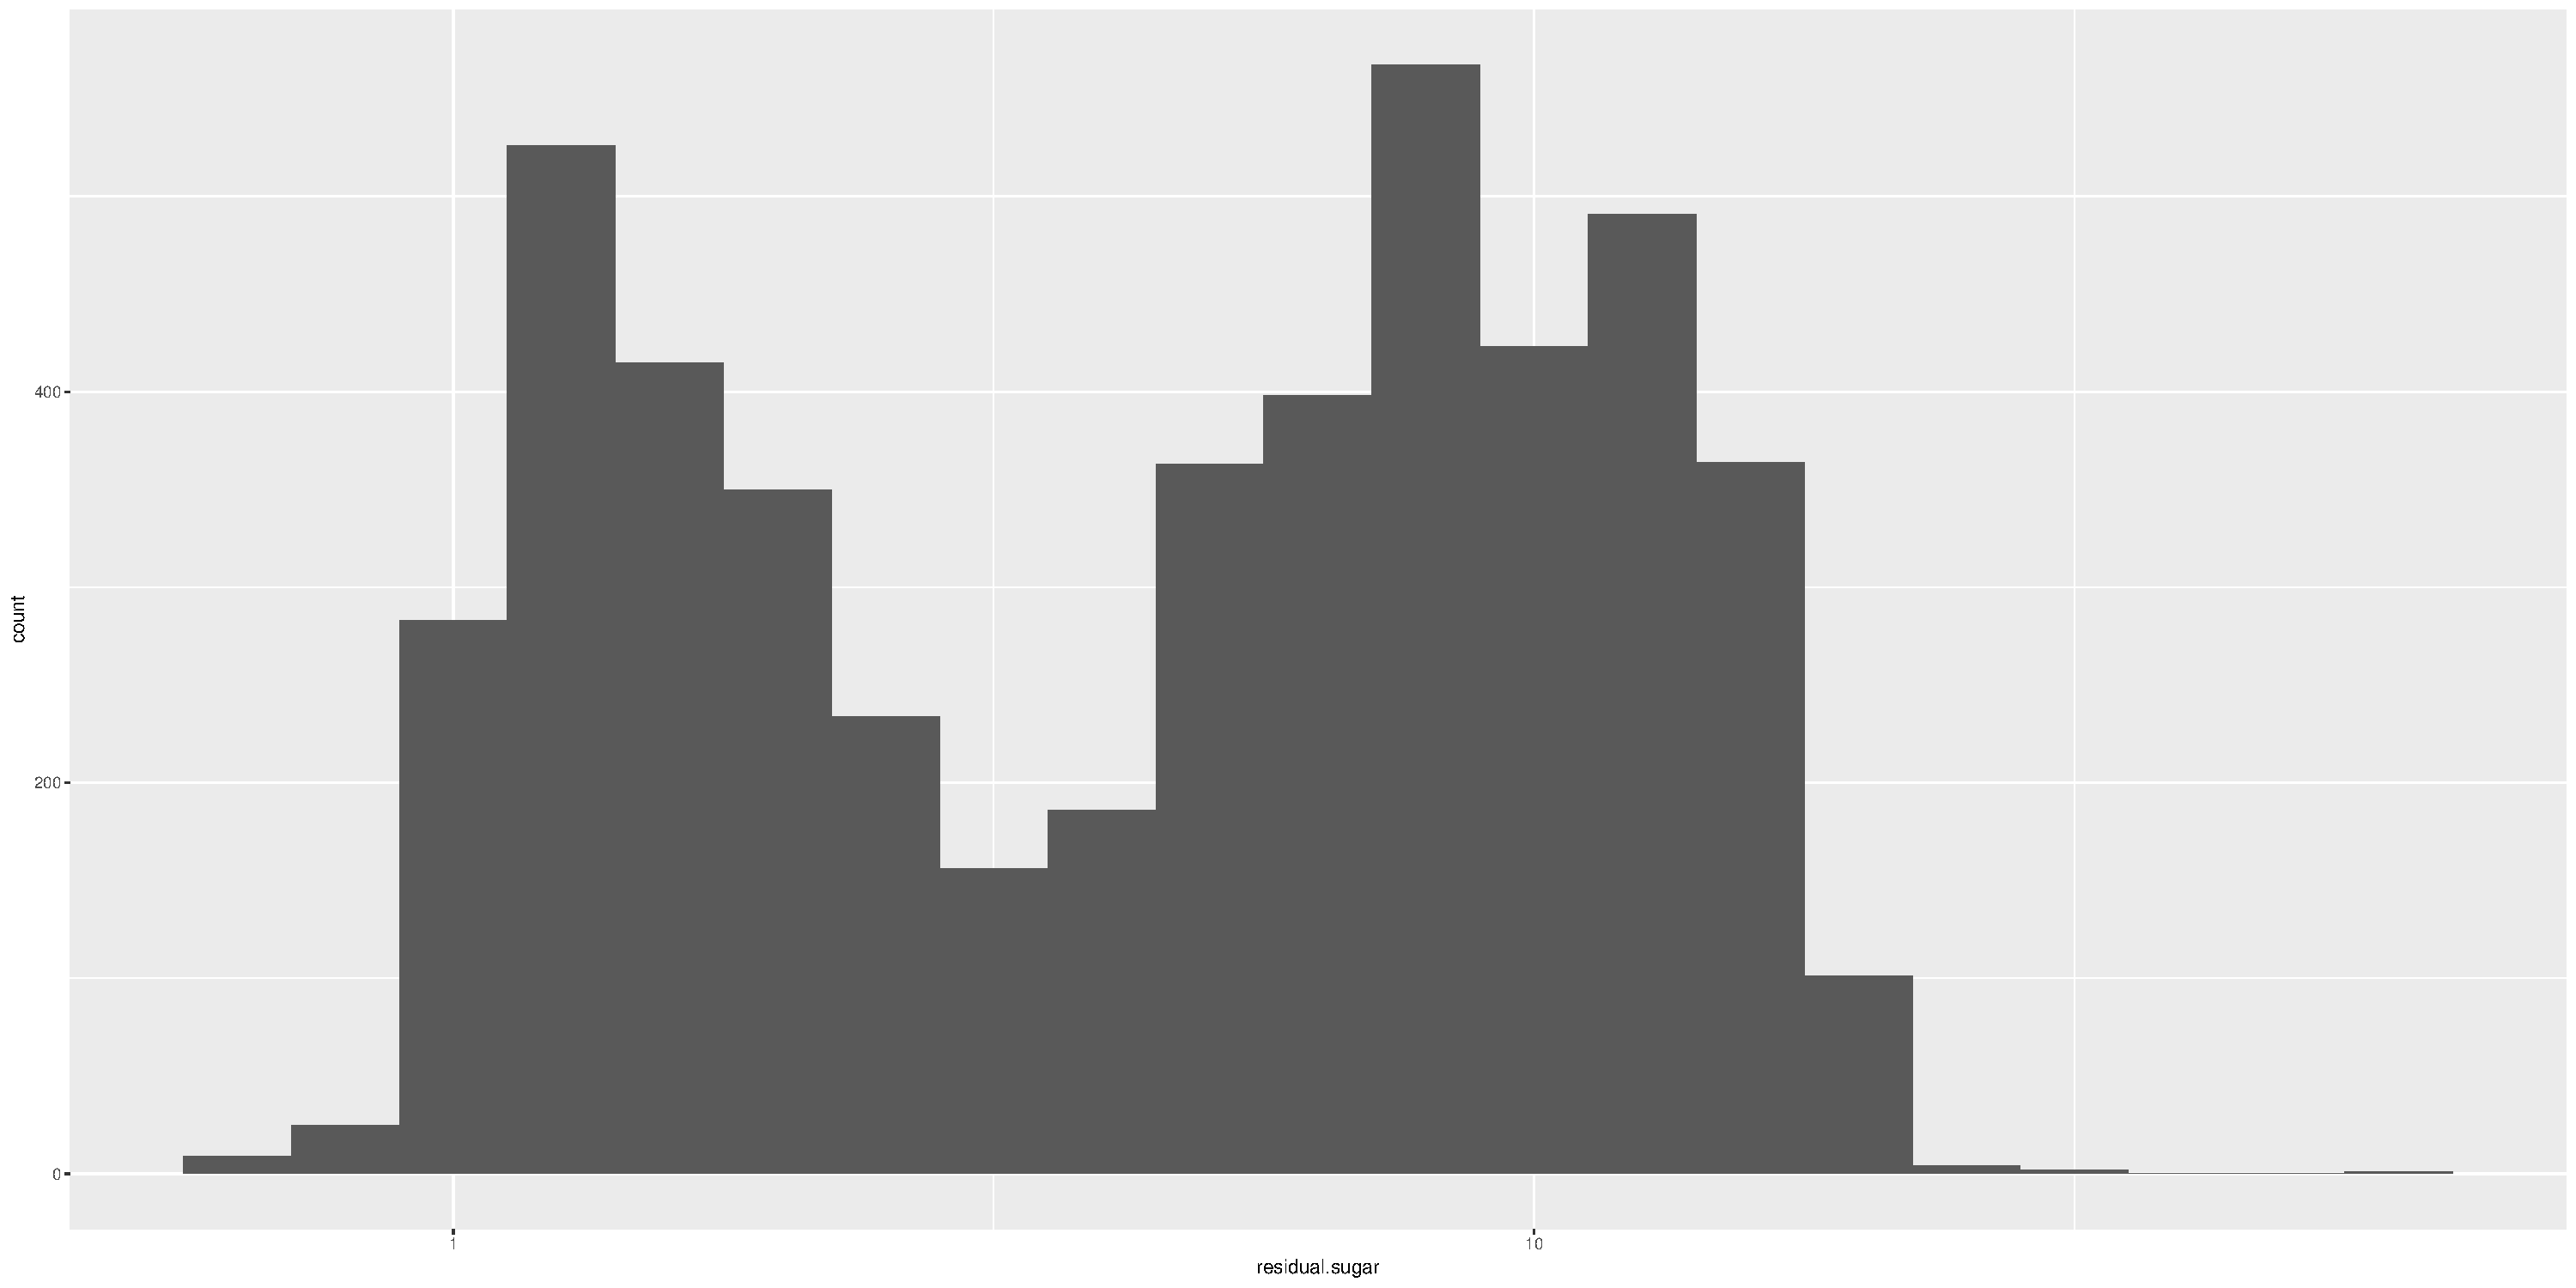
\includegraphics{White_wine_quality_files/figure-latex/unnamed-chunk-11-1.pdf}

The distribution is still skewed to the right after trimming the top 1\%
of data

\paragraph{Chlorides}\label{chlorides}

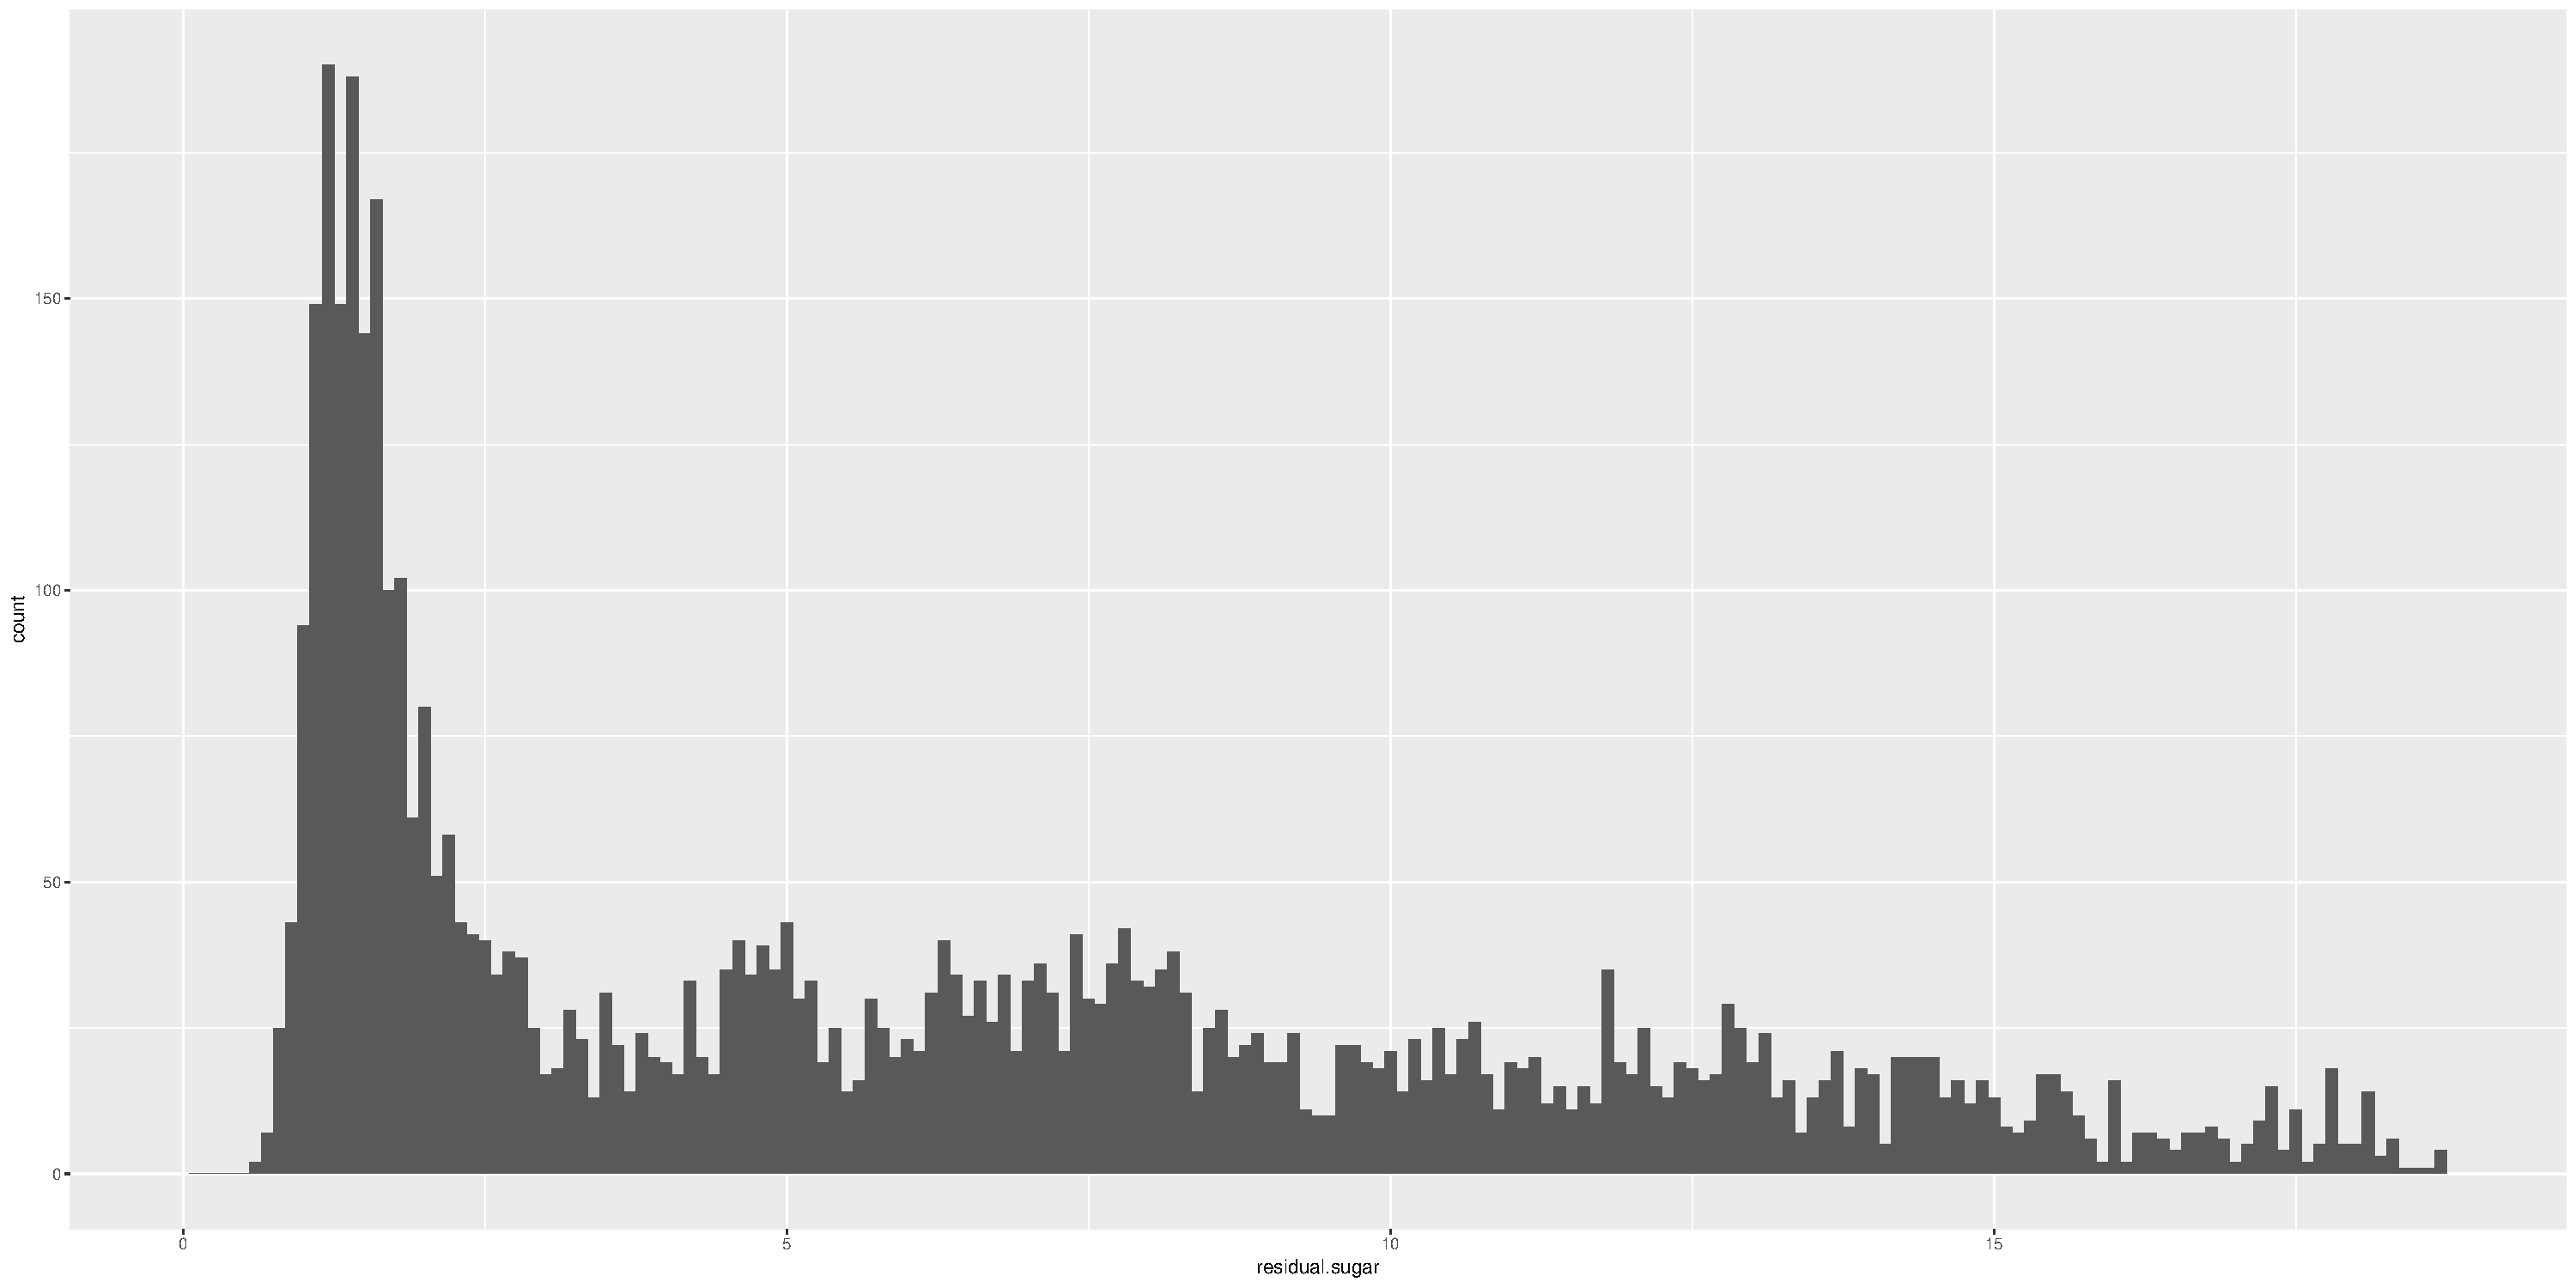
\includegraphics{White_wine_quality_files/figure-latex/unnamed-chunk-12-1.pdf}

The distribution of chloride values looks skewed to the right with a
thin and long tail on the right

Let us trim the top 3\% of chloride values and see how our data looks

\begin{verbatim}
## Warning: Removed 147 rows containing non-finite values (stat_bin).
\end{verbatim}

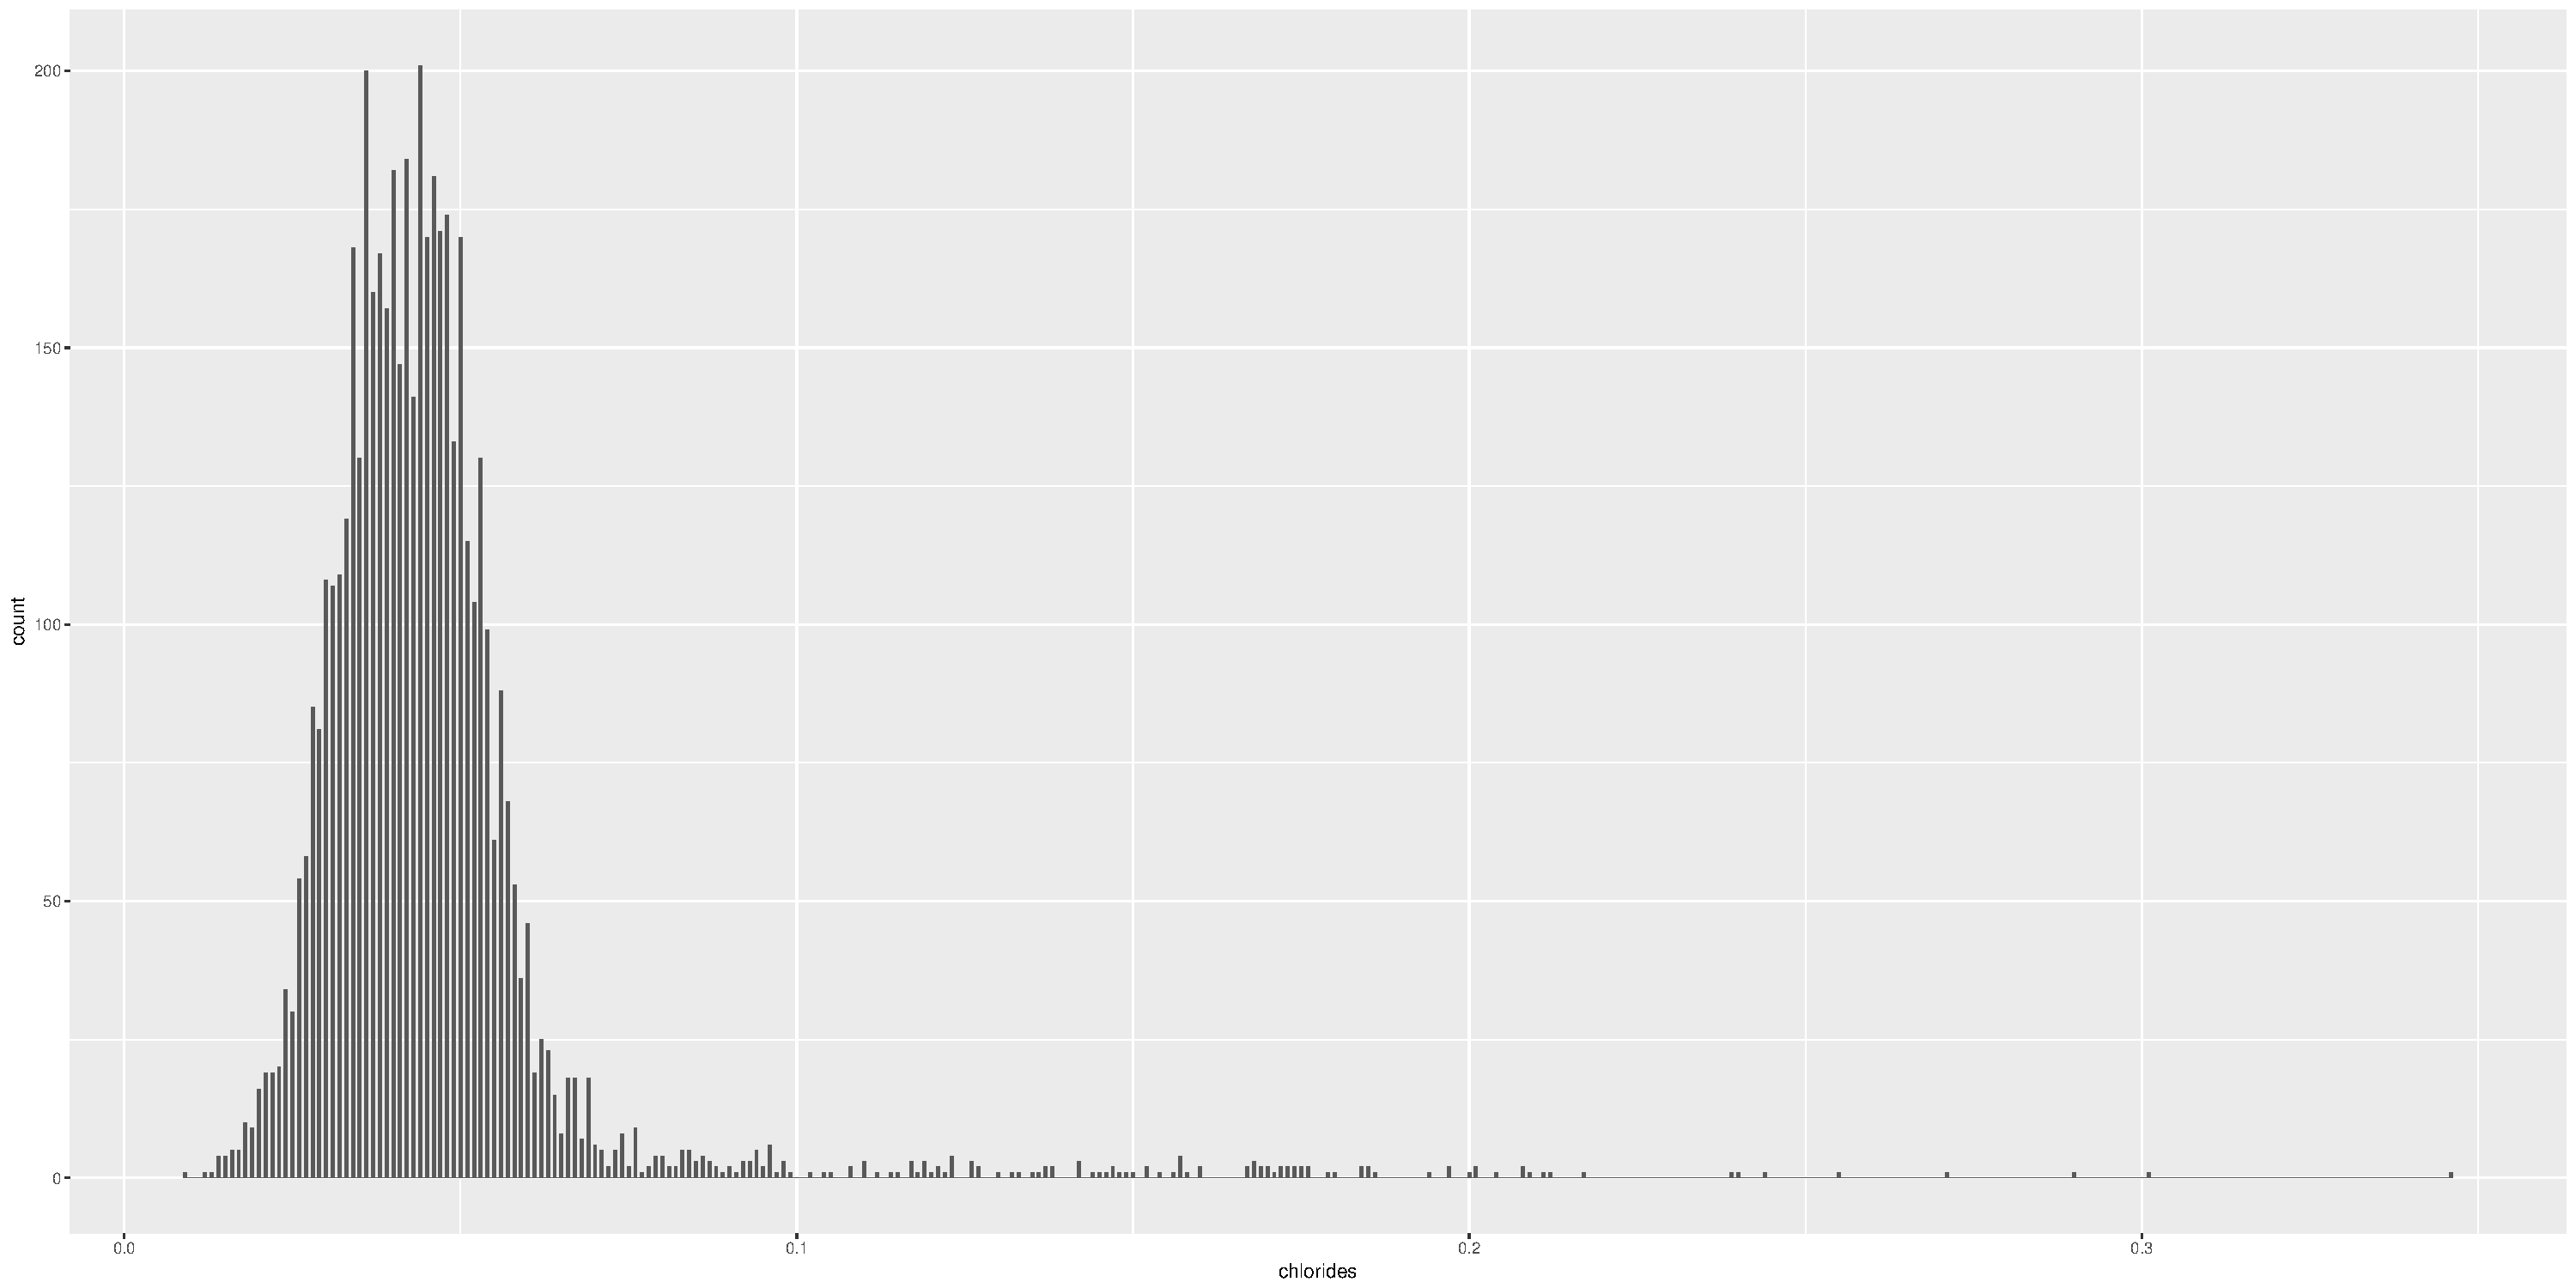
\includegraphics{White_wine_quality_files/figure-latex/unnamed-chunk-13-1.pdf}

Now the data looks a little closer to normal distribution. But it might
not be a good idea to lose 3\% of the data

\paragraph{Free Sulphur dioxide}\label{free-sulphur-dioxide}

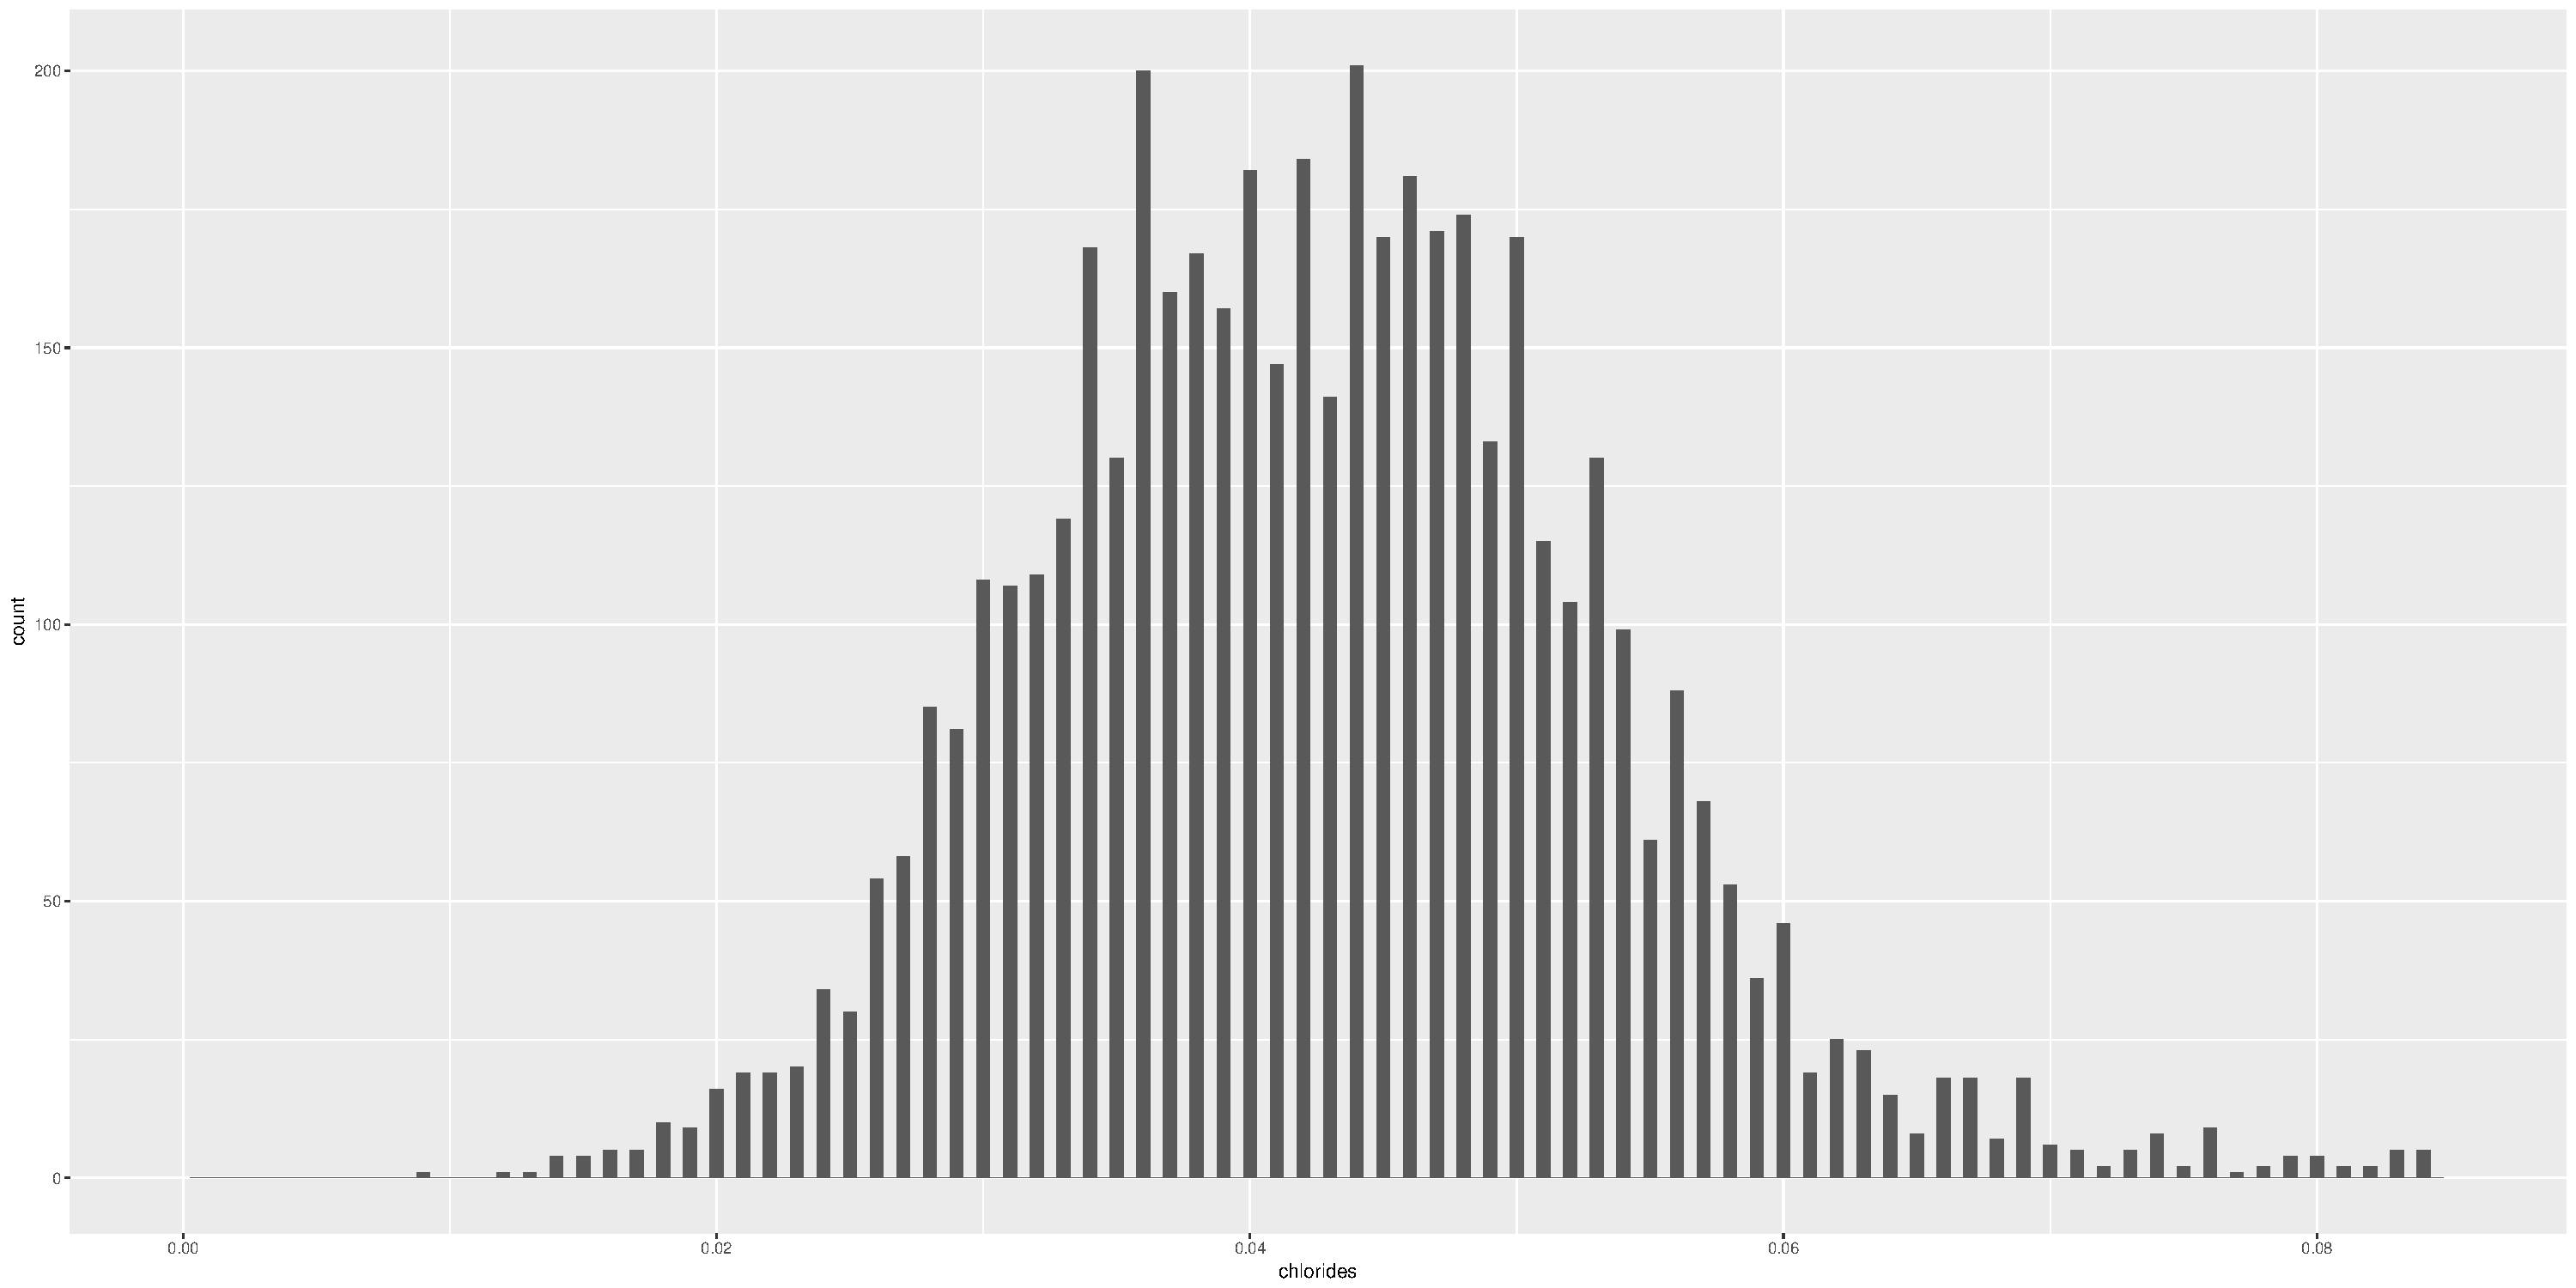
\includegraphics{White_wine_quality_files/figure-latex/unnamed-chunk-14-1.pdf}
The distribution of free sulphurdioxide looks skewed to the right with
an outlier point at 289

\paragraph{Total Sulphur dioxide}\label{total-sulphur-dioxide}

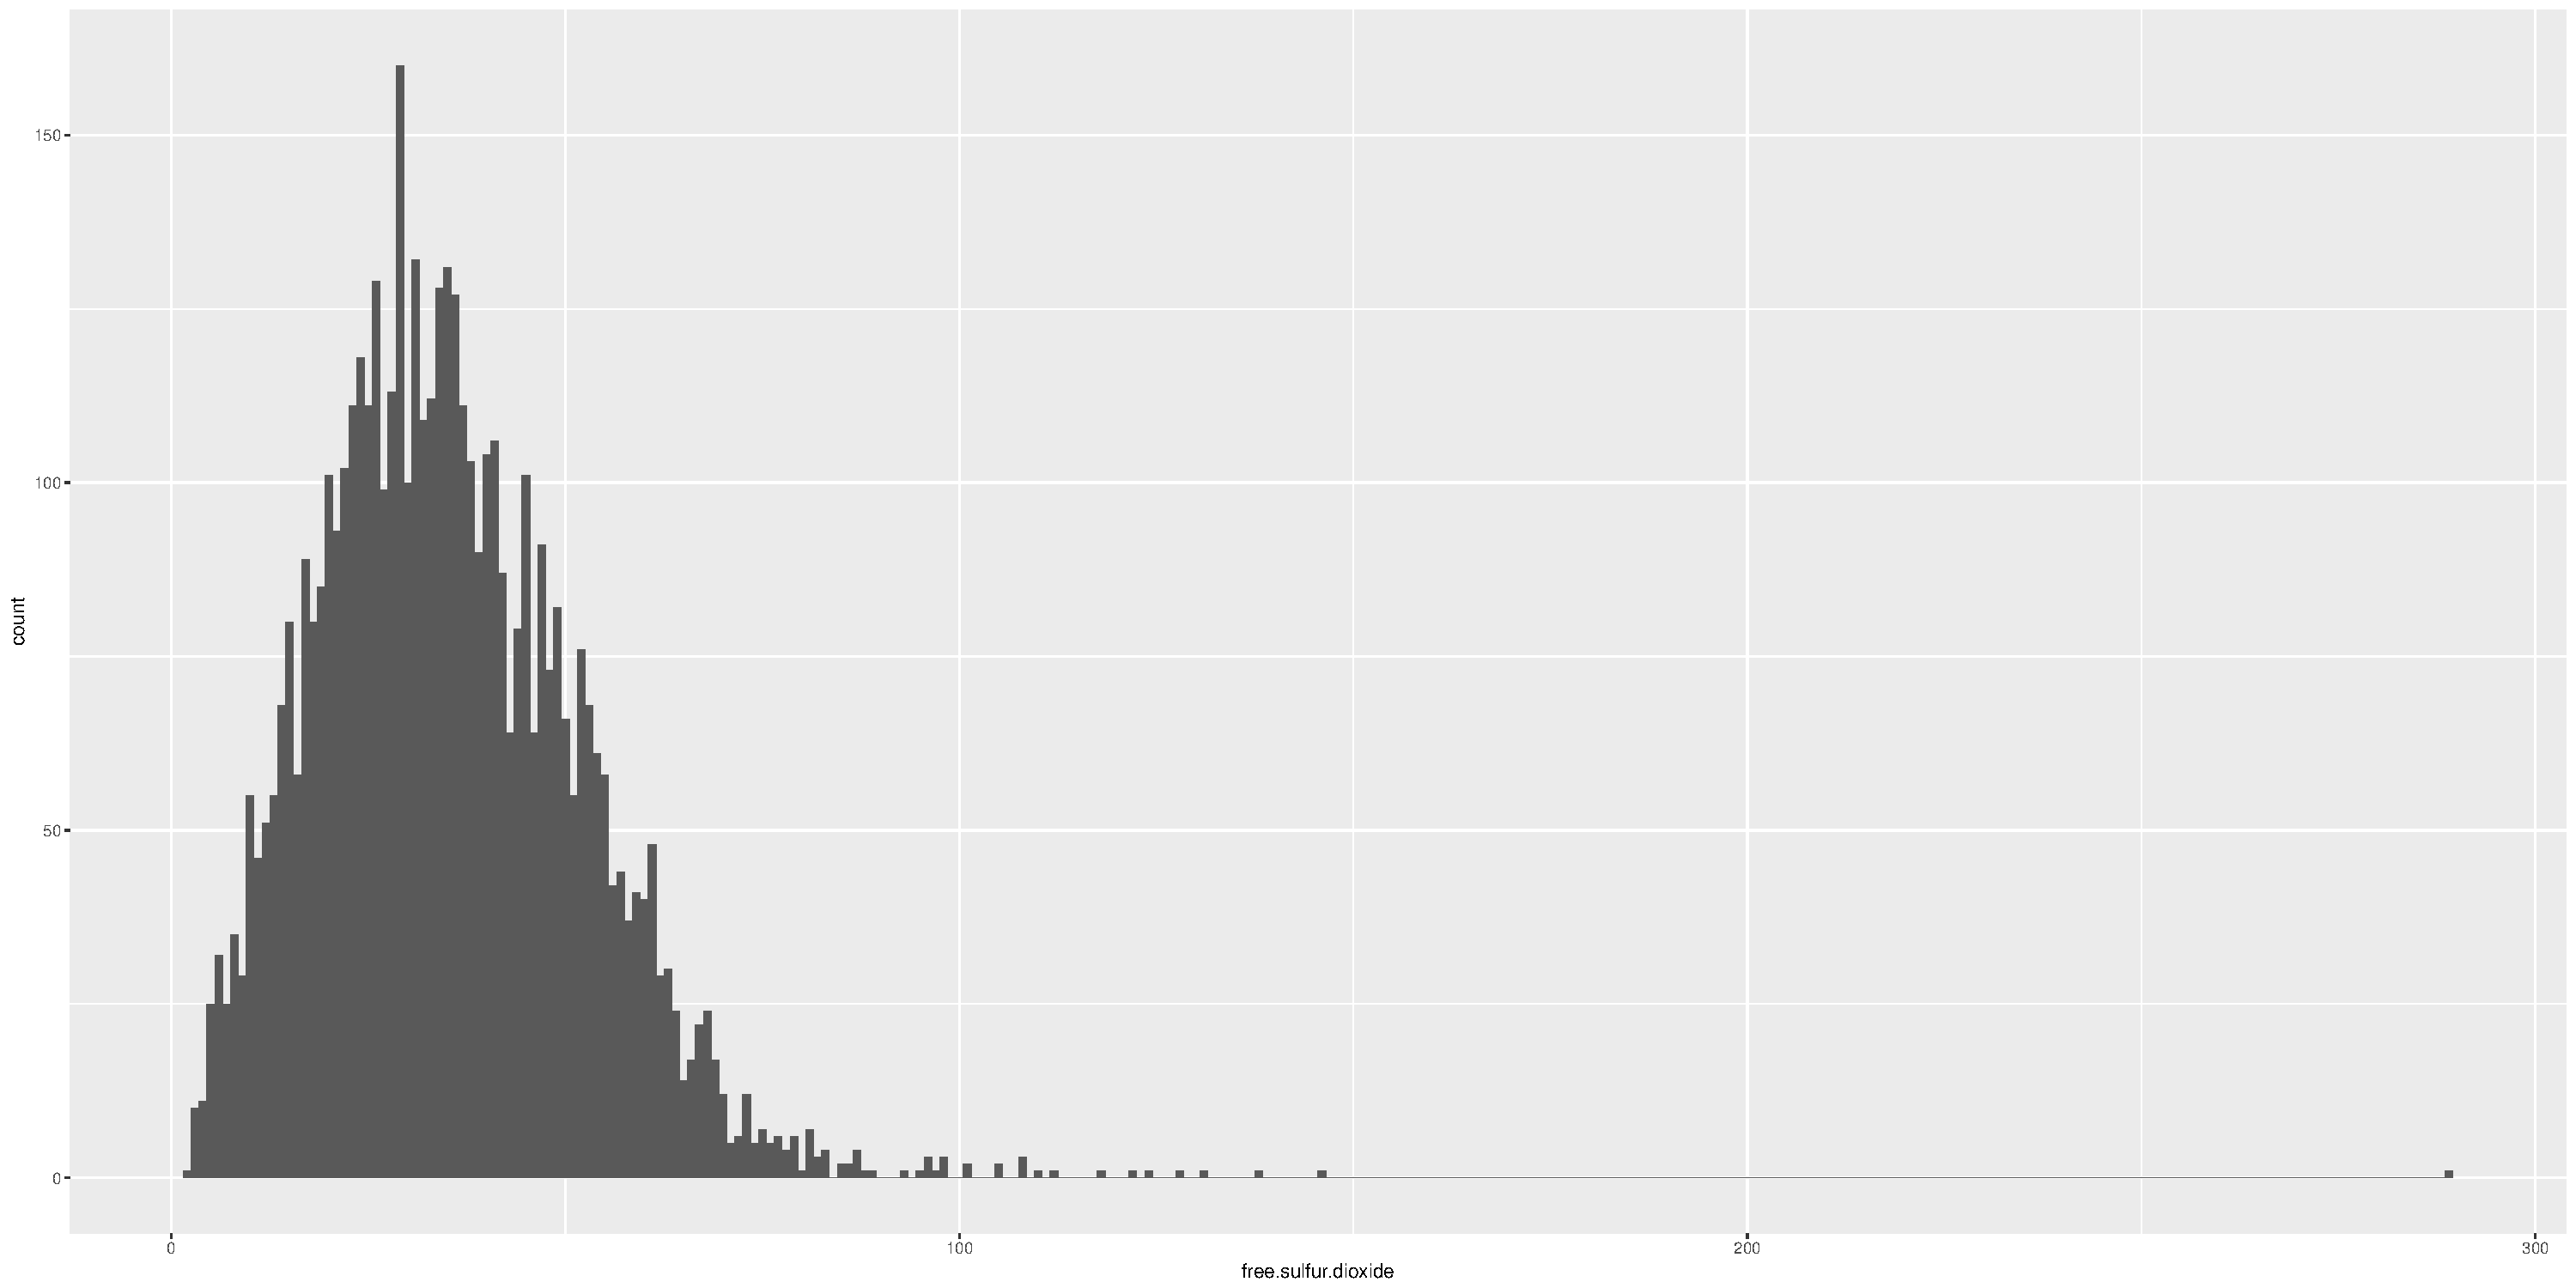
\includegraphics{White_wine_quality_files/figure-latex/unnamed-chunk-15-1.pdf}
The bulk of total sulphur dioxide data looks normally distributed with a
few outliers on the right

\paragraph{Density}\label{density}

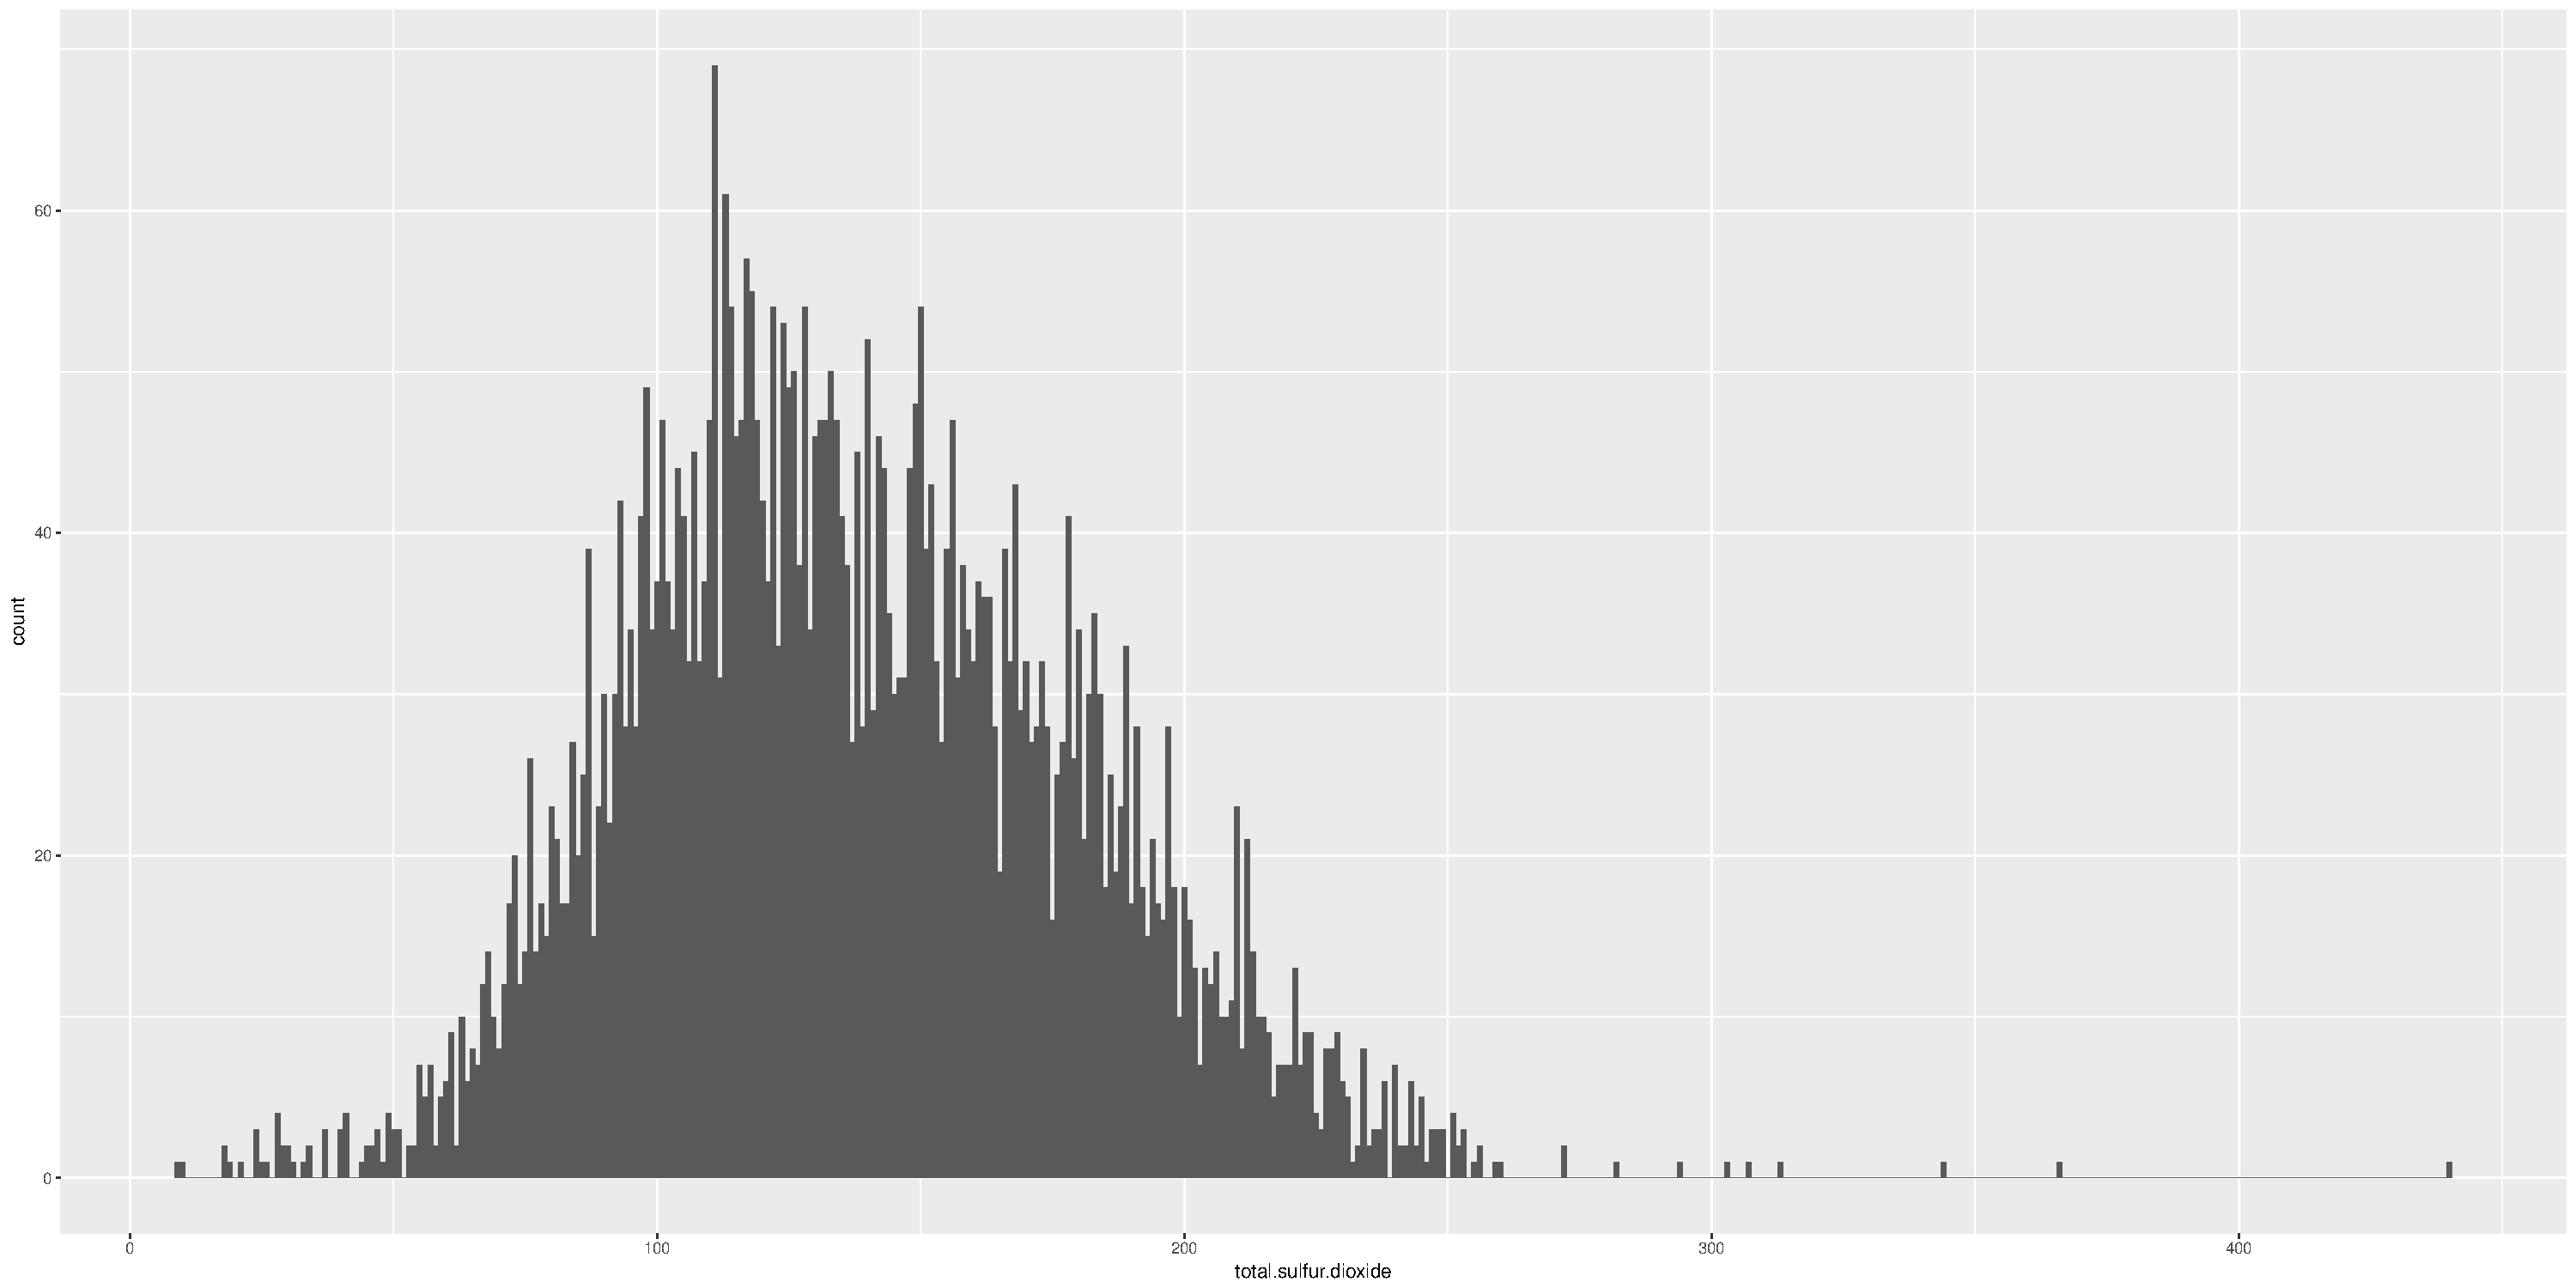
\includegraphics{White_wine_quality_files/figure-latex/unnamed-chunk-16-1.pdf}
The distribution of density looks almost normally distributed Few wines
seem to have a density greater than 1 - most probably they should be
outliers

\paragraph{pH}\label{ph}

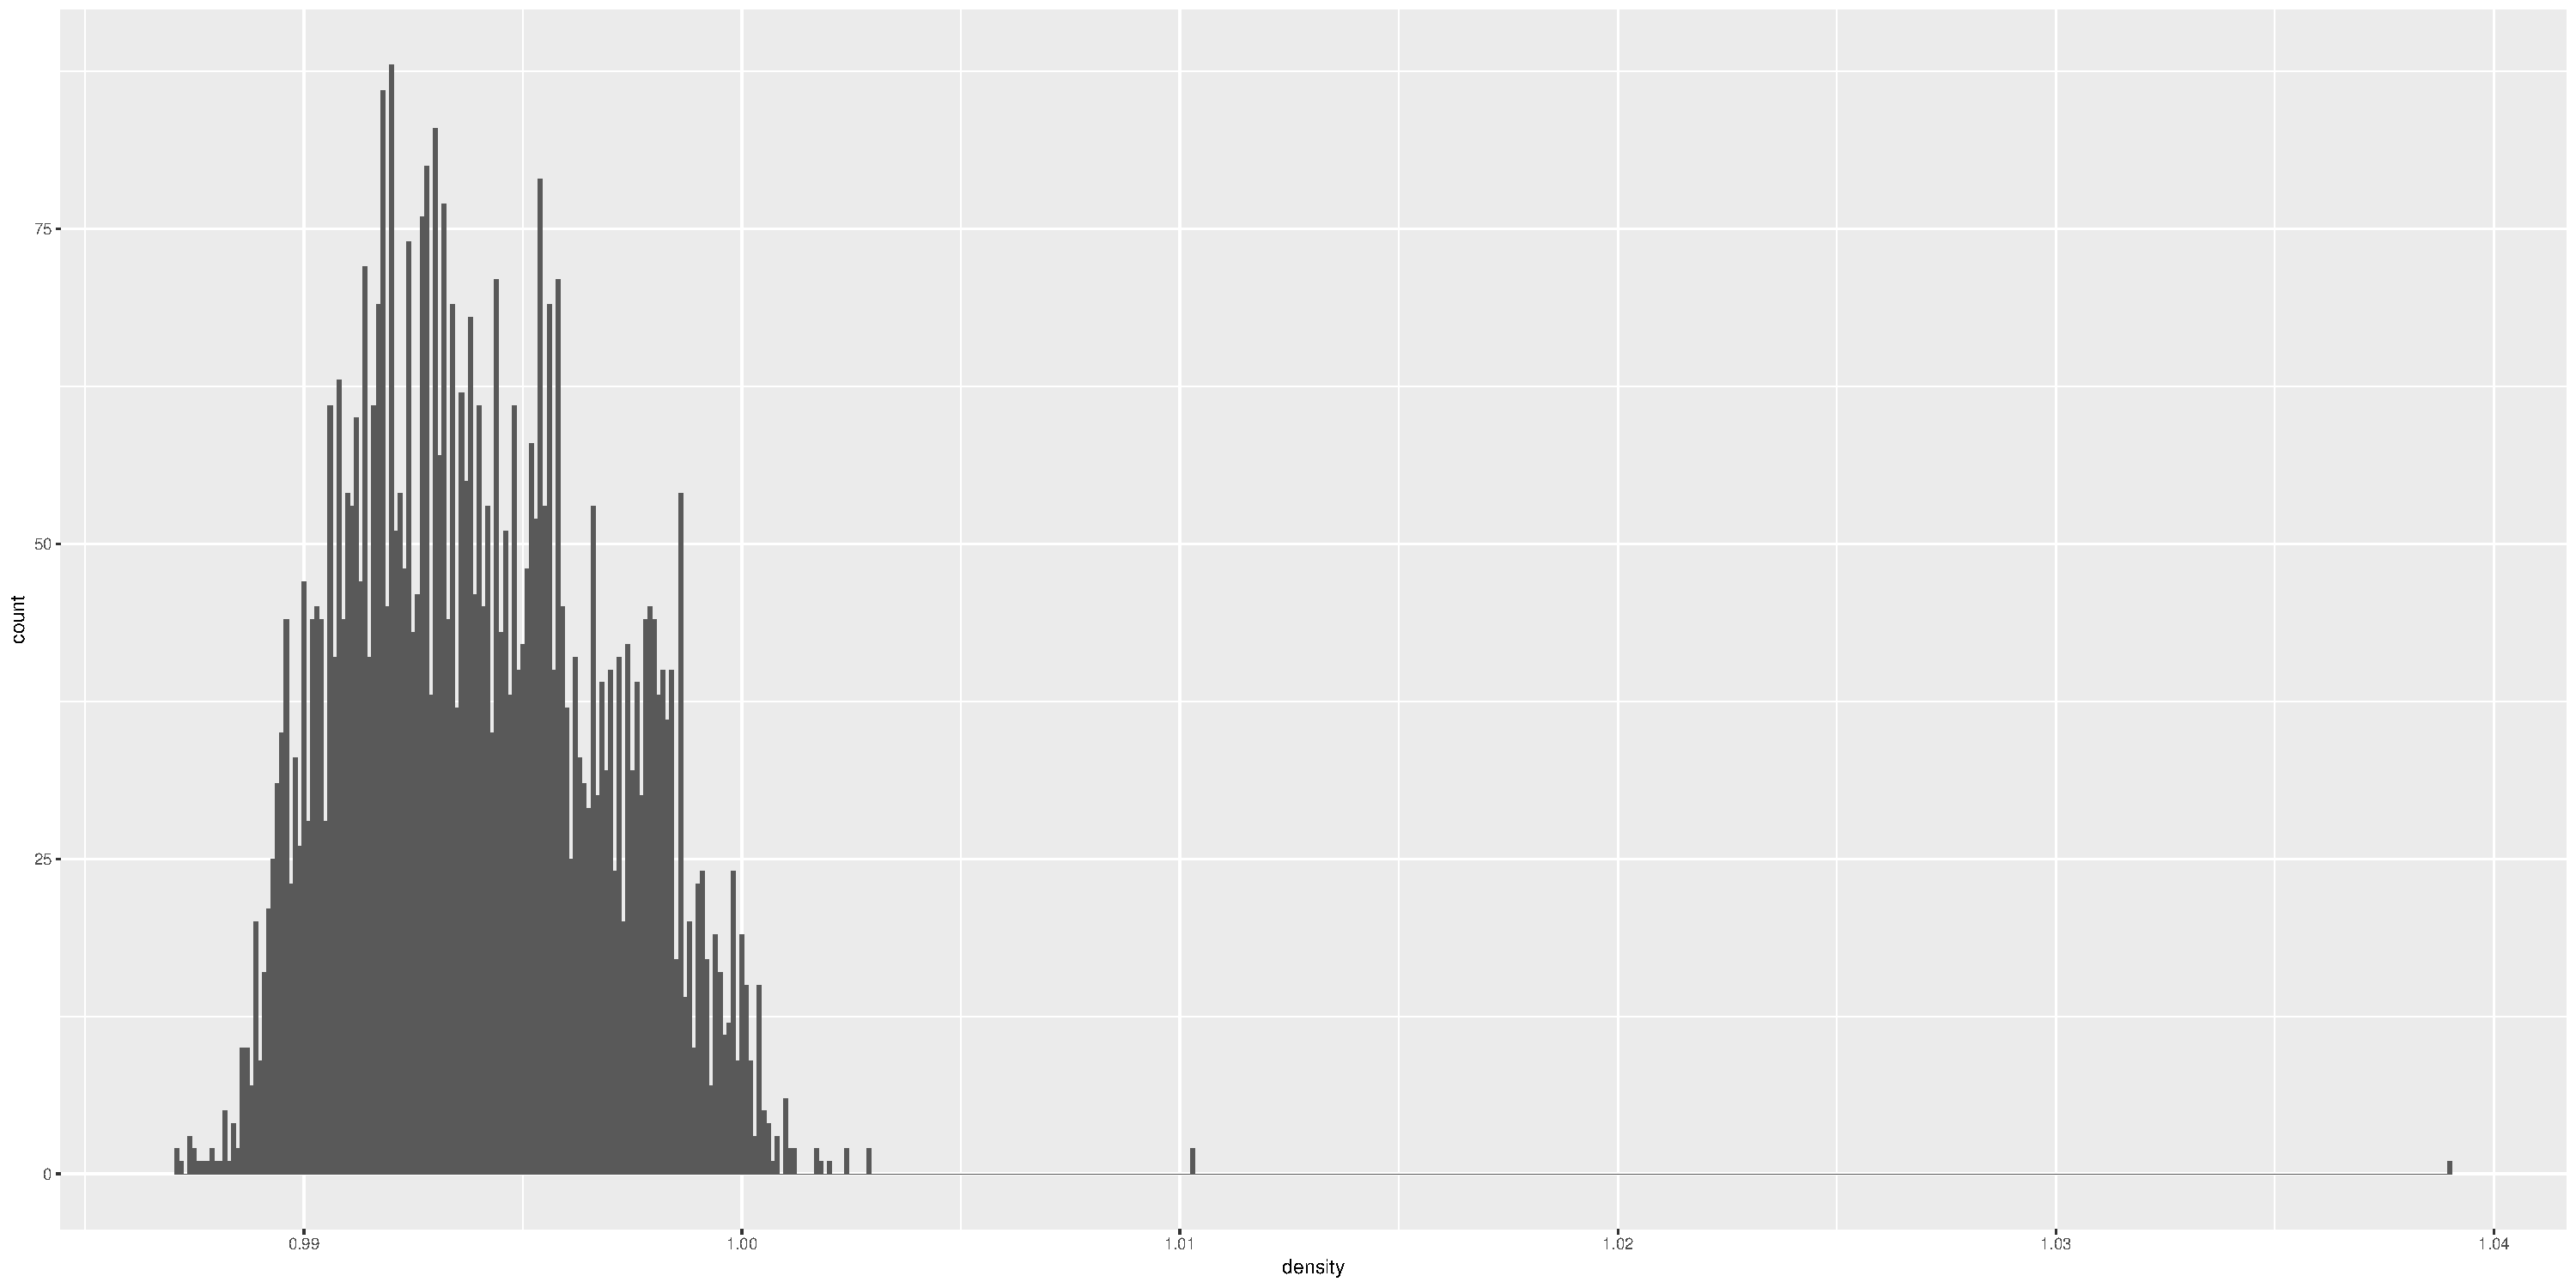
\includegraphics{White_wine_quality_files/figure-latex/unnamed-chunk-17-1.pdf}

pH values appear to be normally distributed. From domain knowledge, we
can expect pH / acidity to be key factors influencing the quality of
wine

\paragraph{Sulphates}\label{sulphates}

\includegraphics{White_wine_quality_files/figure-latex/unnamed-chunk-18-1.pdf}

The distribution of sulphates appears skewed to the right

Let us transform the sulphates axis on a log10 scale

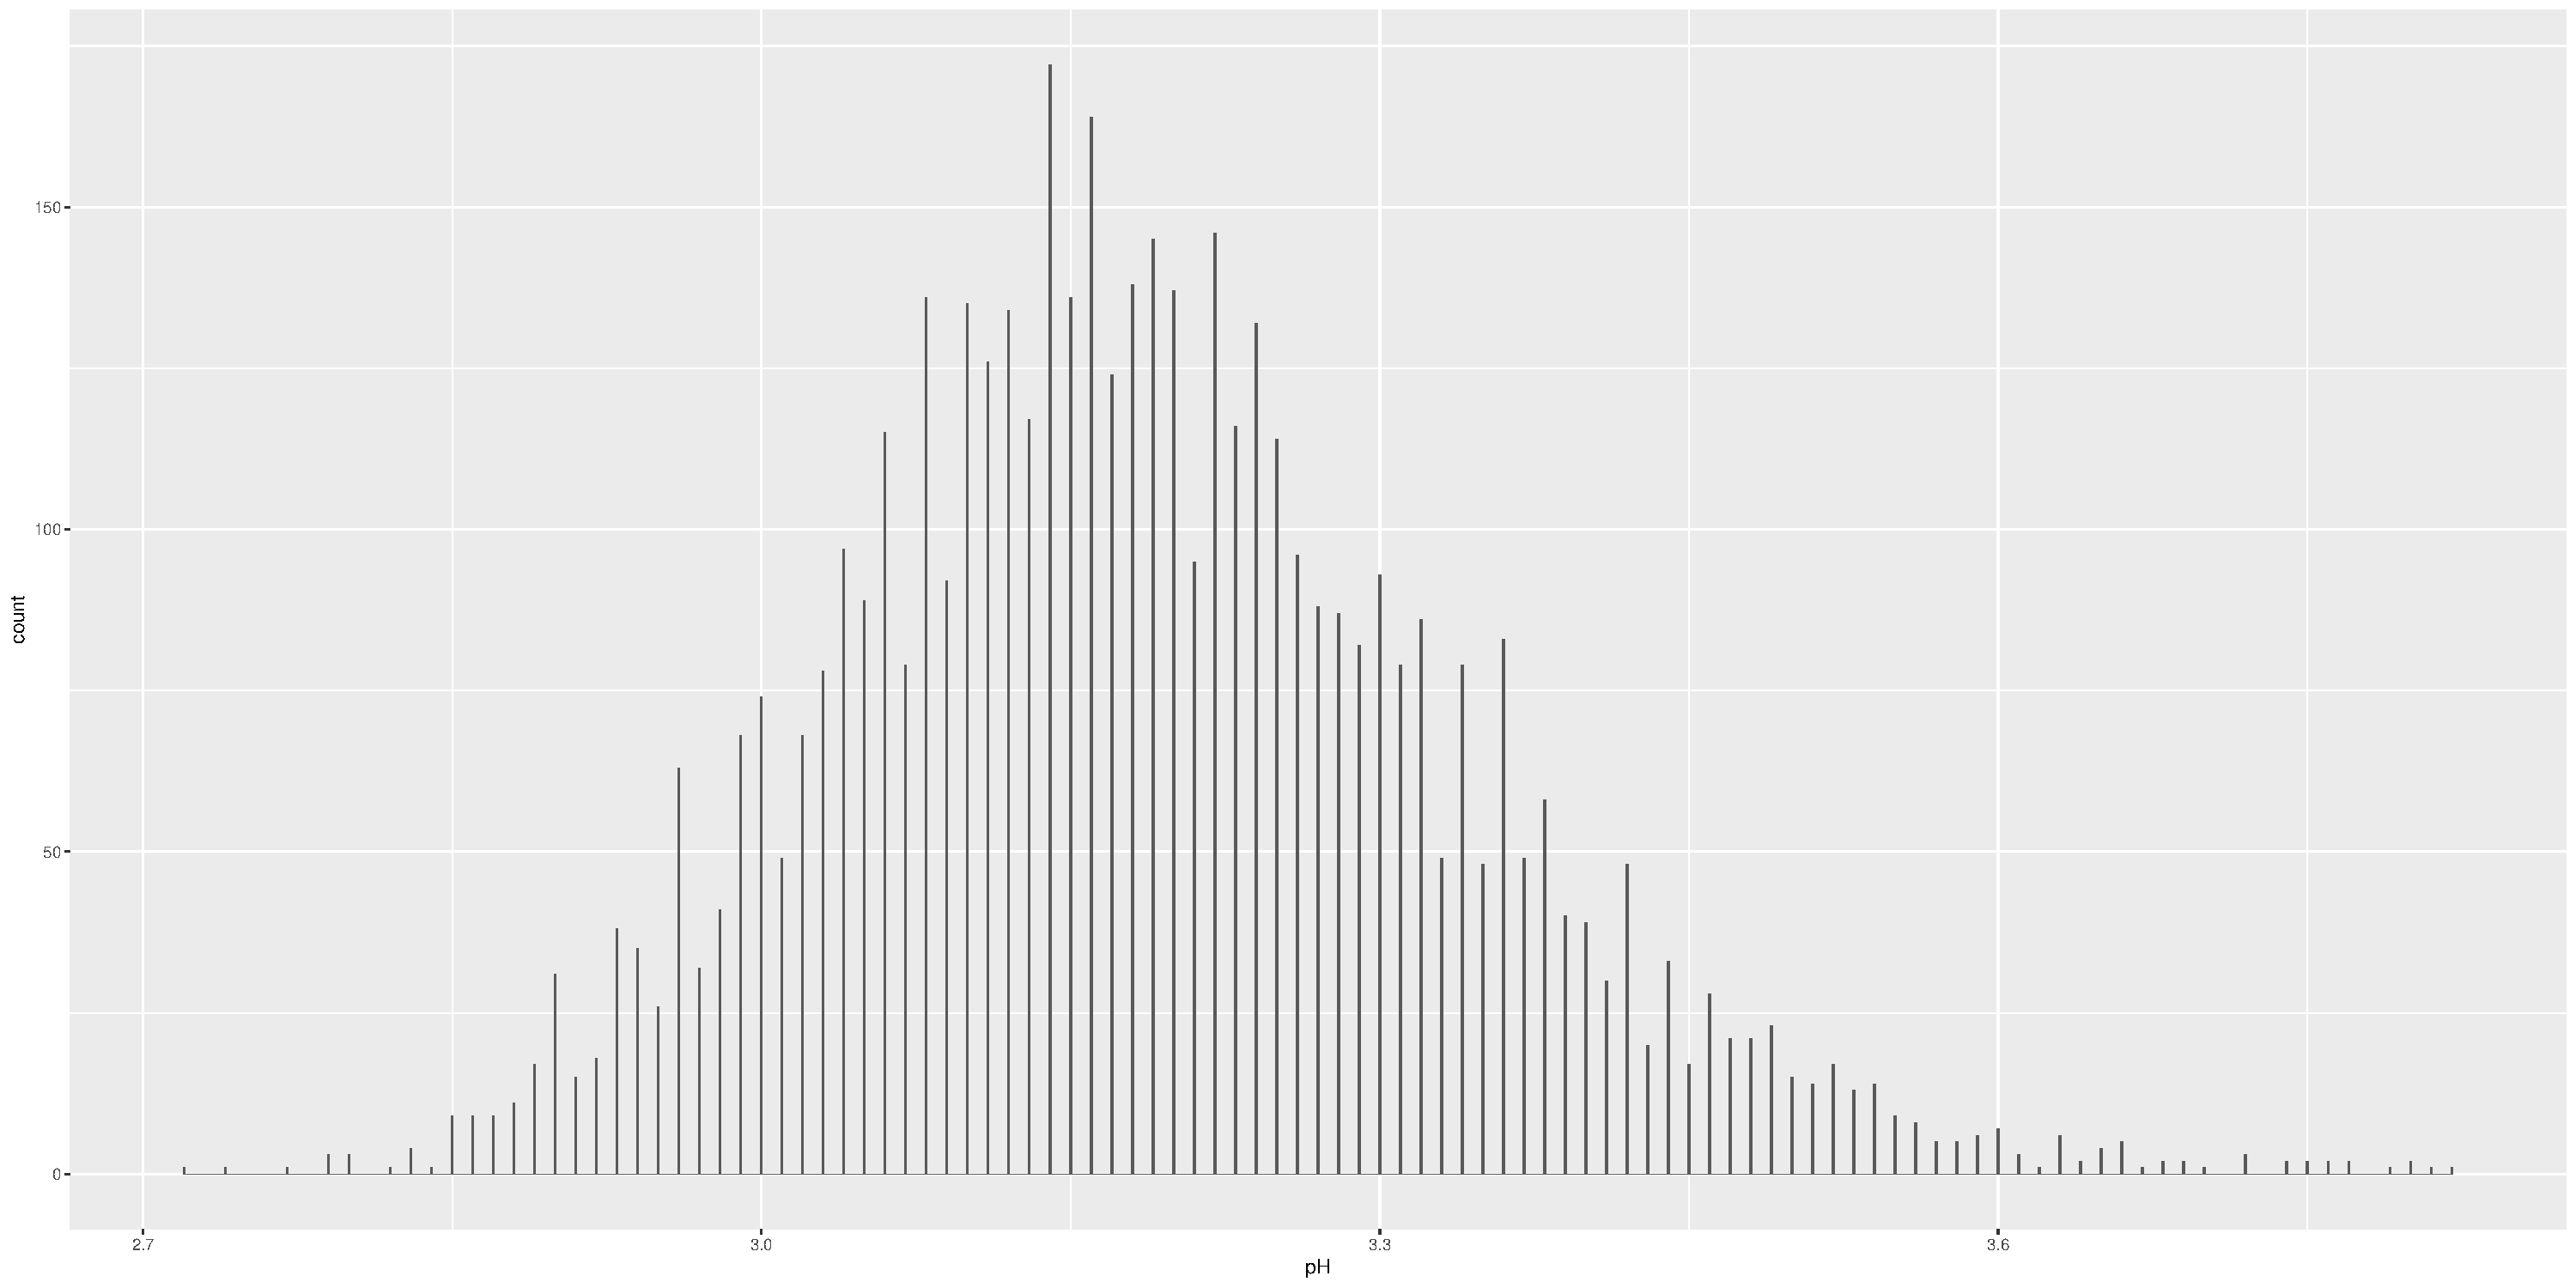
\includegraphics{White_wine_quality_files/figure-latex/unnamed-chunk-19-1.pdf}
The distribution of sulphates appears closer to normal distribution with
a log10 transformation

\paragraph{Alcohol}\label{alcohol}

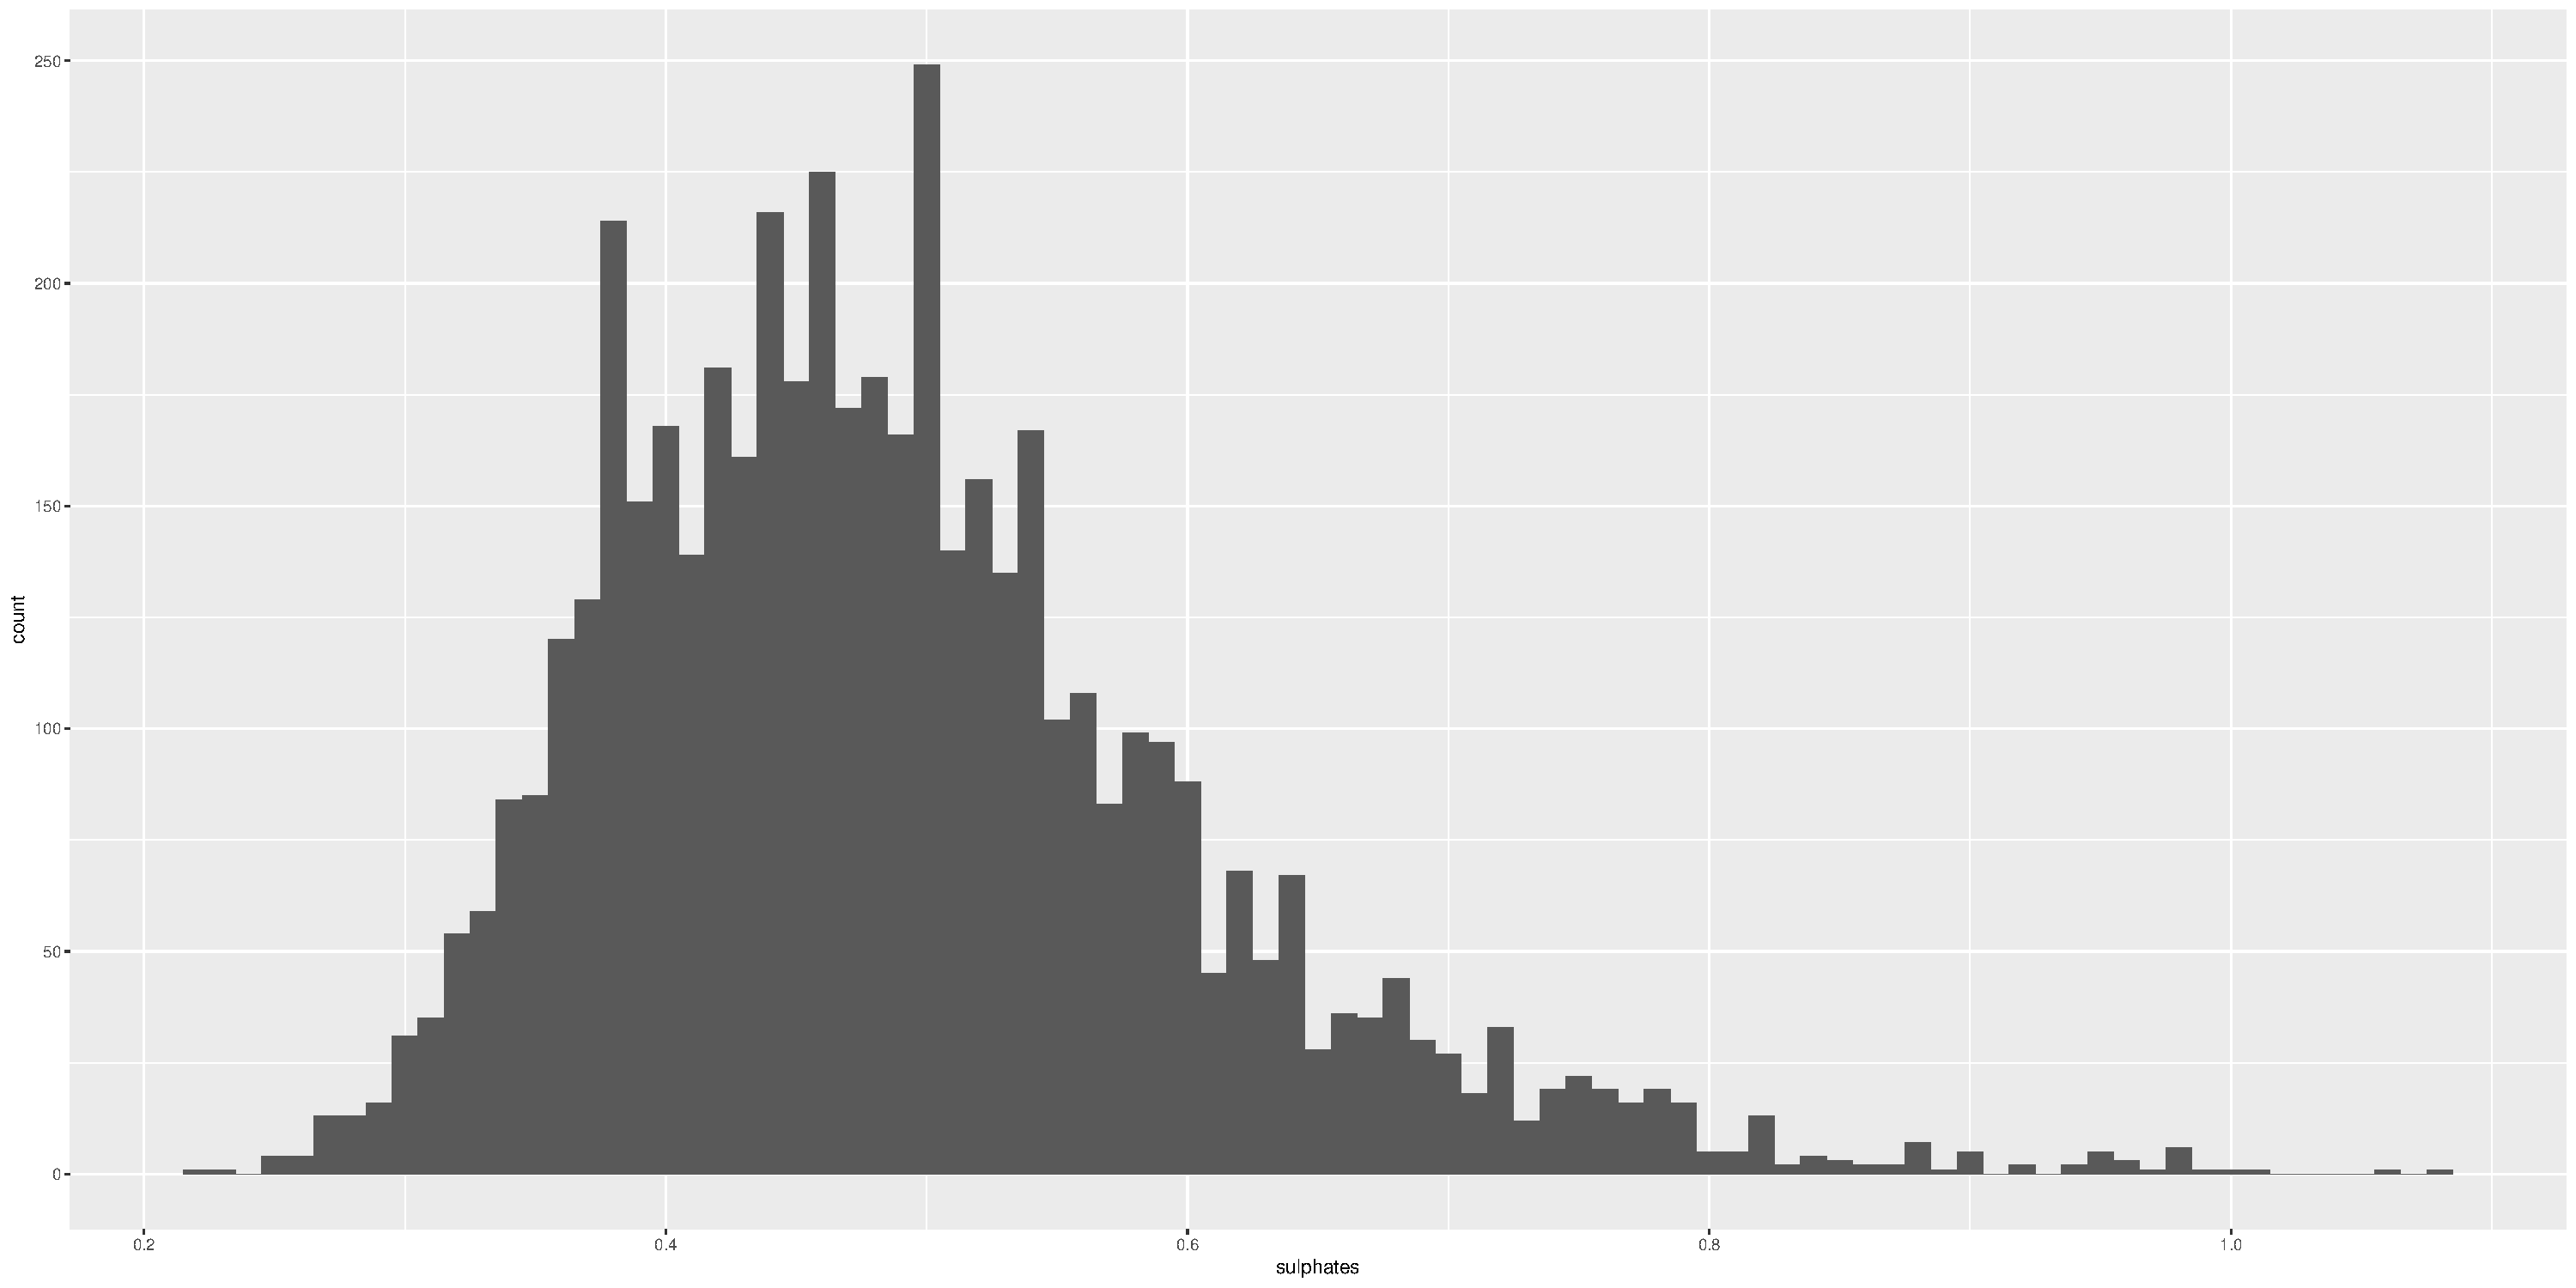
\includegraphics{White_wine_quality_files/figure-latex/unnamed-chunk-20-1.pdf}

The histogram for alcohol level does not look normally distributed.

let us try a log10 transform on alcohol level data

\begin{verbatim}
## `stat_bin()` using `bins = 30`. Pick better value with `binwidth`.
\end{verbatim}

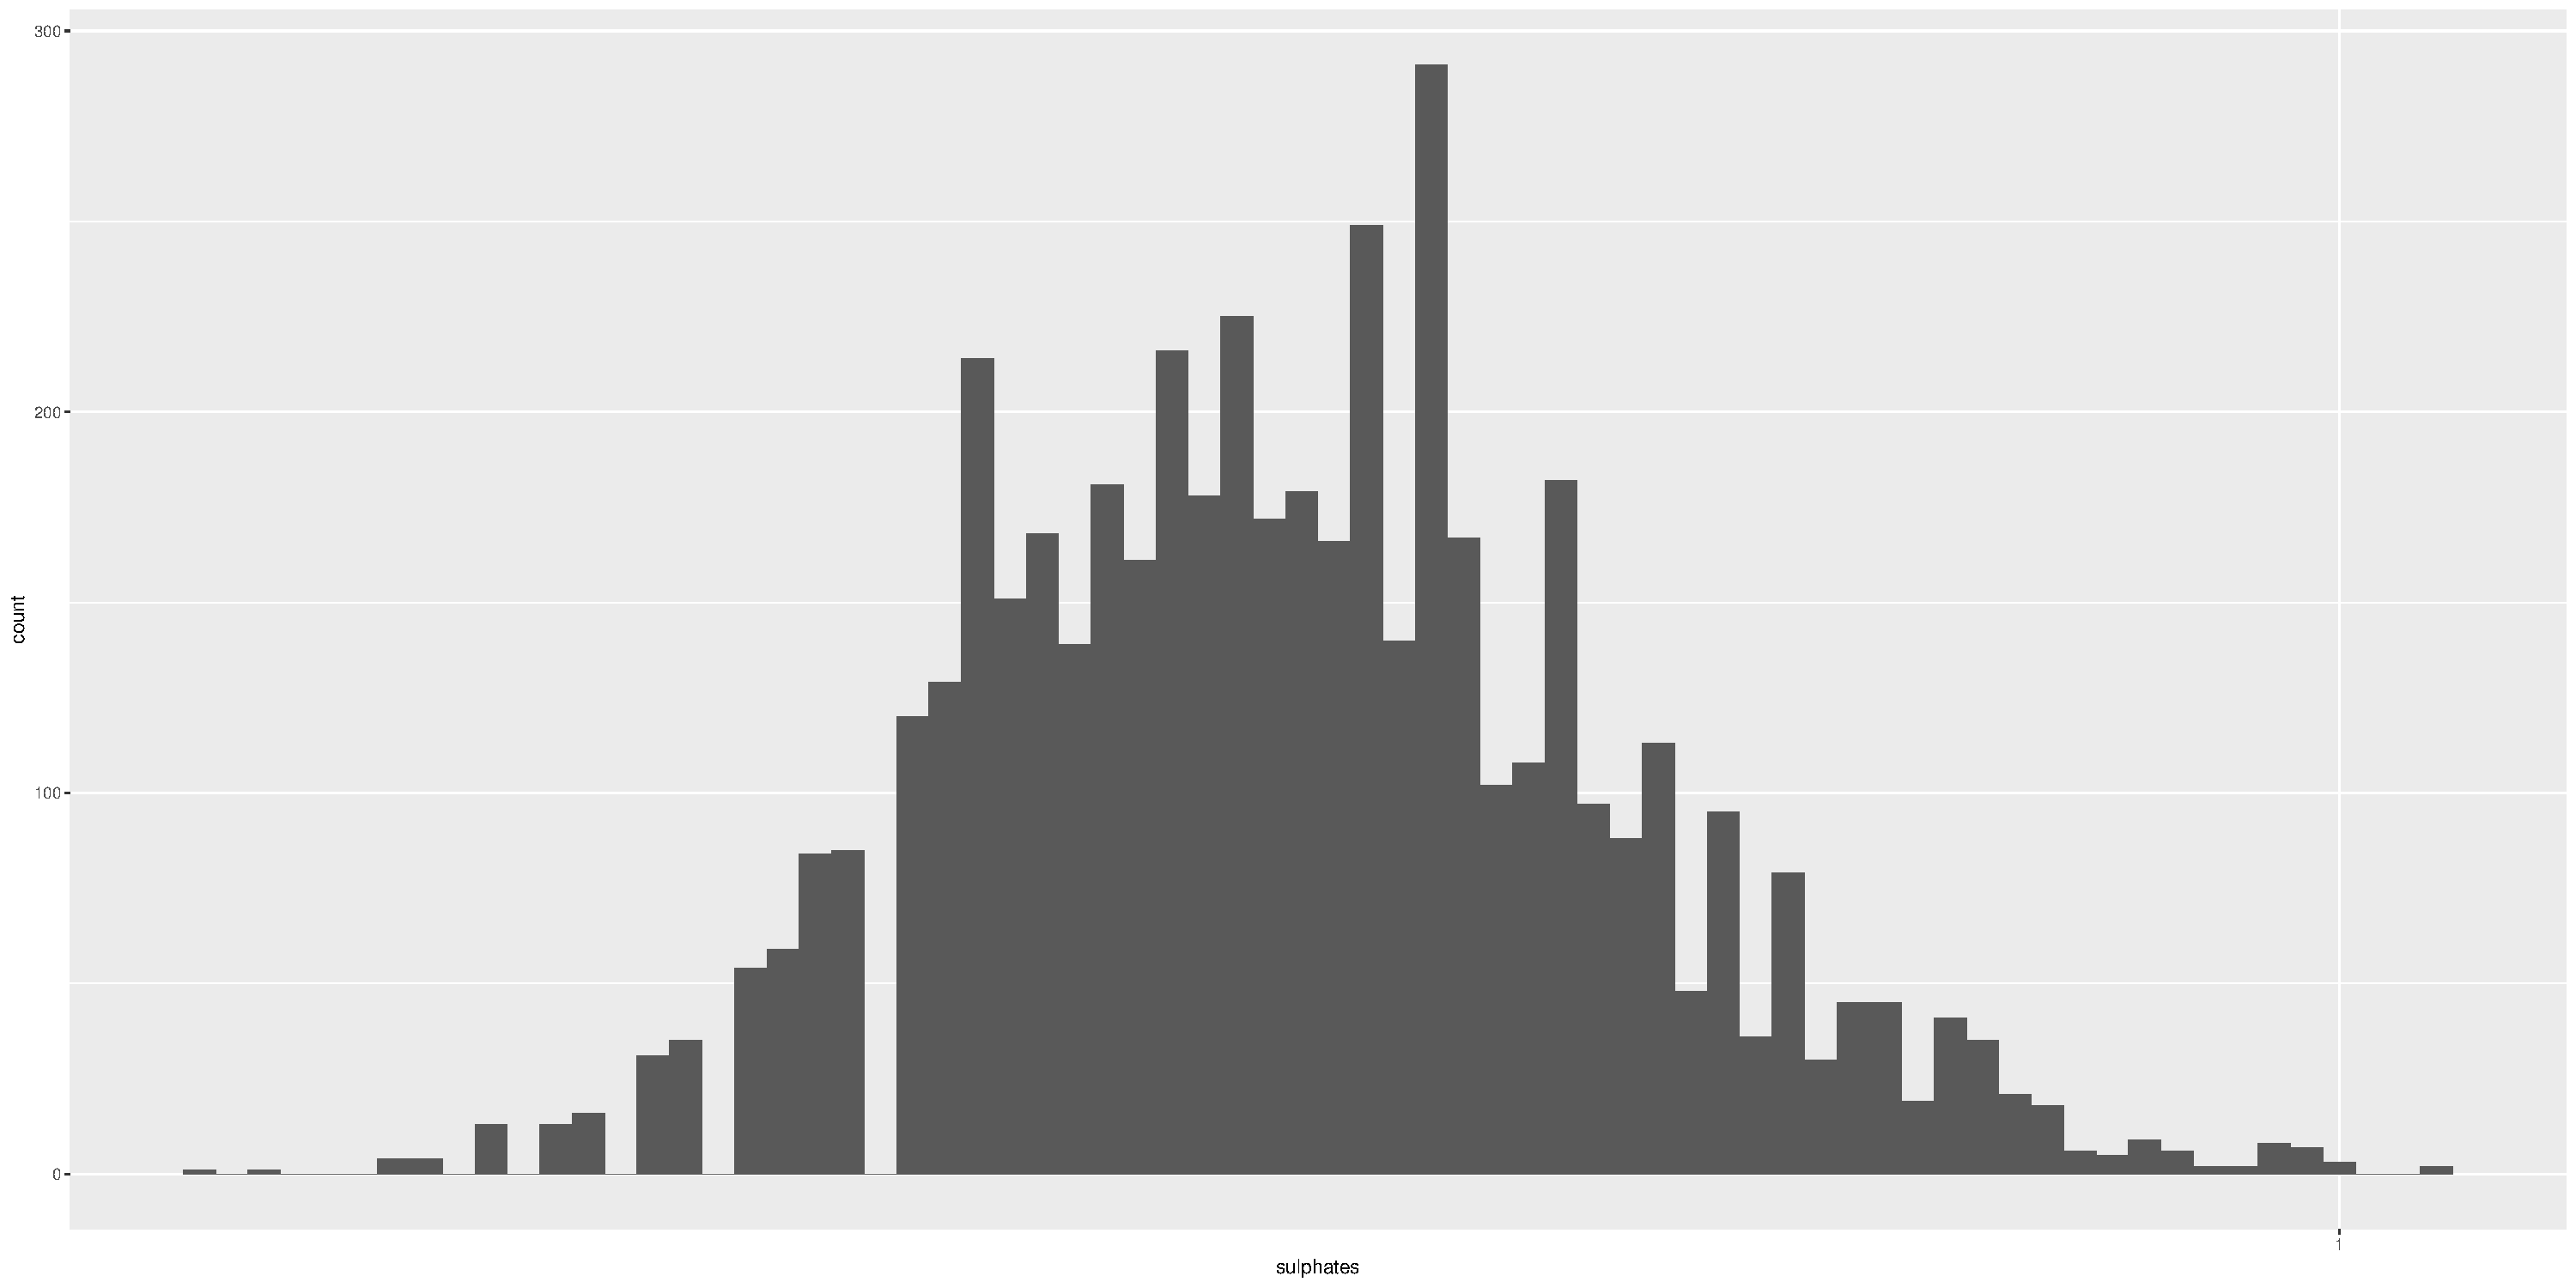
\includegraphics{White_wine_quality_files/figure-latex/unnamed-chunk-21-1.pdf}

Even after the log10 transformation, alcohol level data does not look
normally distributed

Let us try a sqrt transform on the alcohol level data

\begin{verbatim}
## `stat_bin()` using `bins = 30`. Pick better value with `binwidth`.
\end{verbatim}

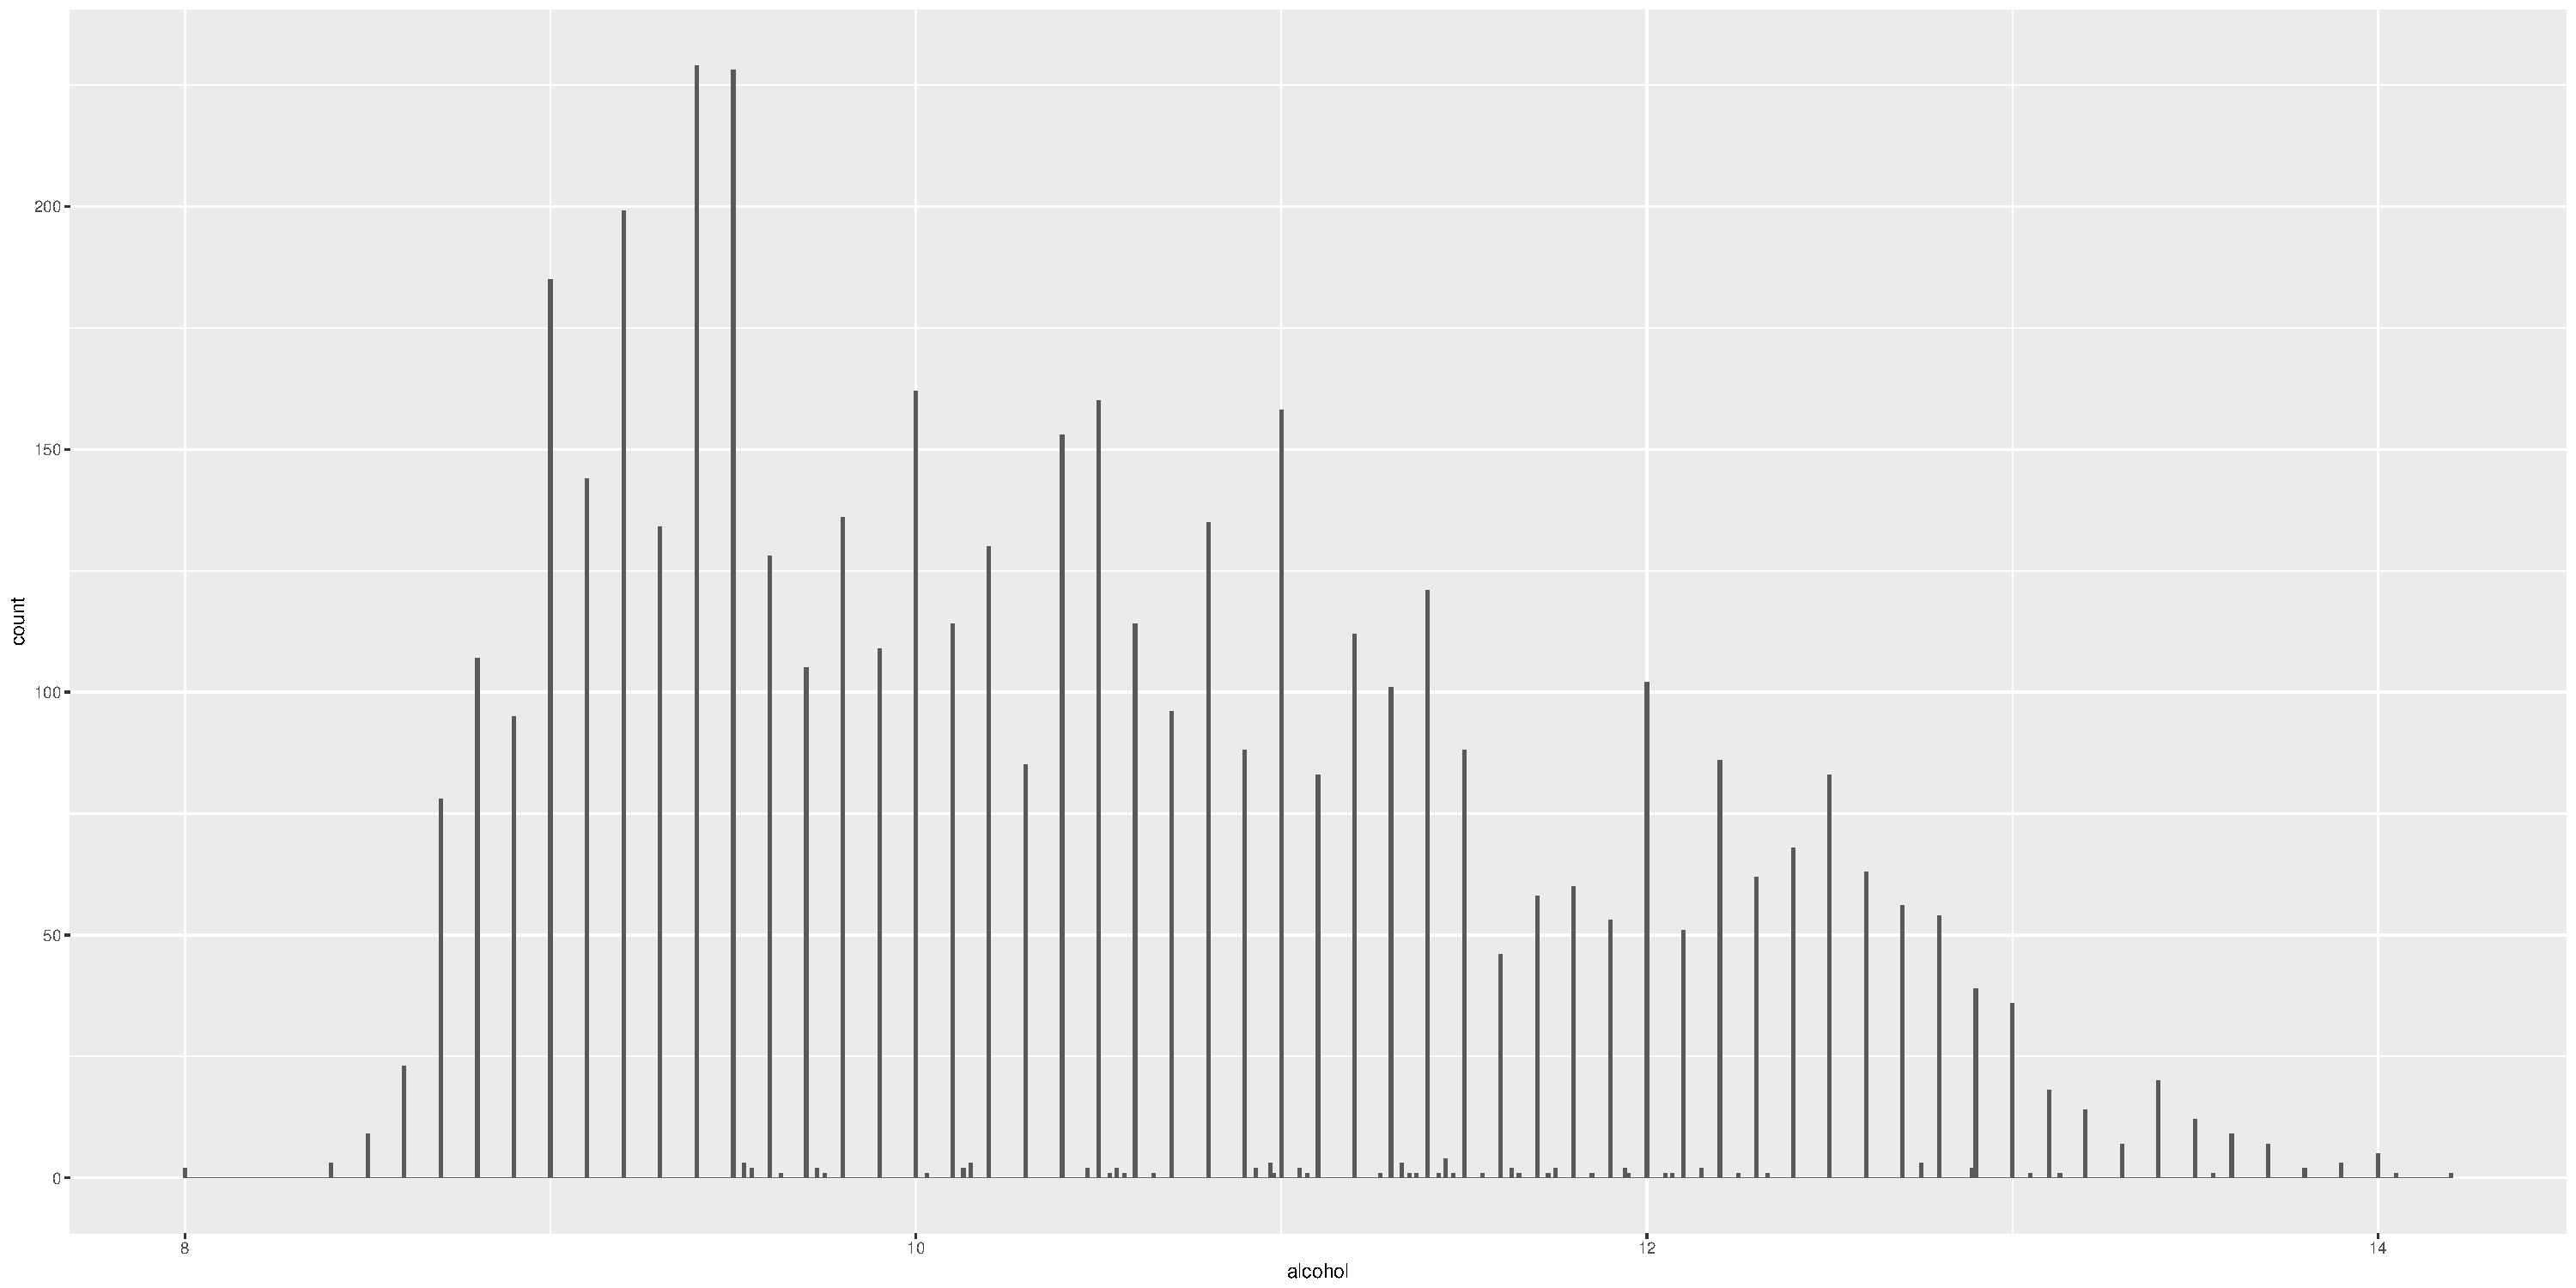
\includegraphics{White_wine_quality_files/figure-latex/unnamed-chunk-22-1.pdf}

The sqrt transformation also doesn't seem to make the alcohol level data
normally distributed

From common knowledge, alcohol levels of wine could be a key influencer
of wine quality

\paragraph{Quality}\label{quality}

\begin{verbatim}
## `stat_bin()` using `bins = 30`. Pick better value with `binwidth`.
\end{verbatim}

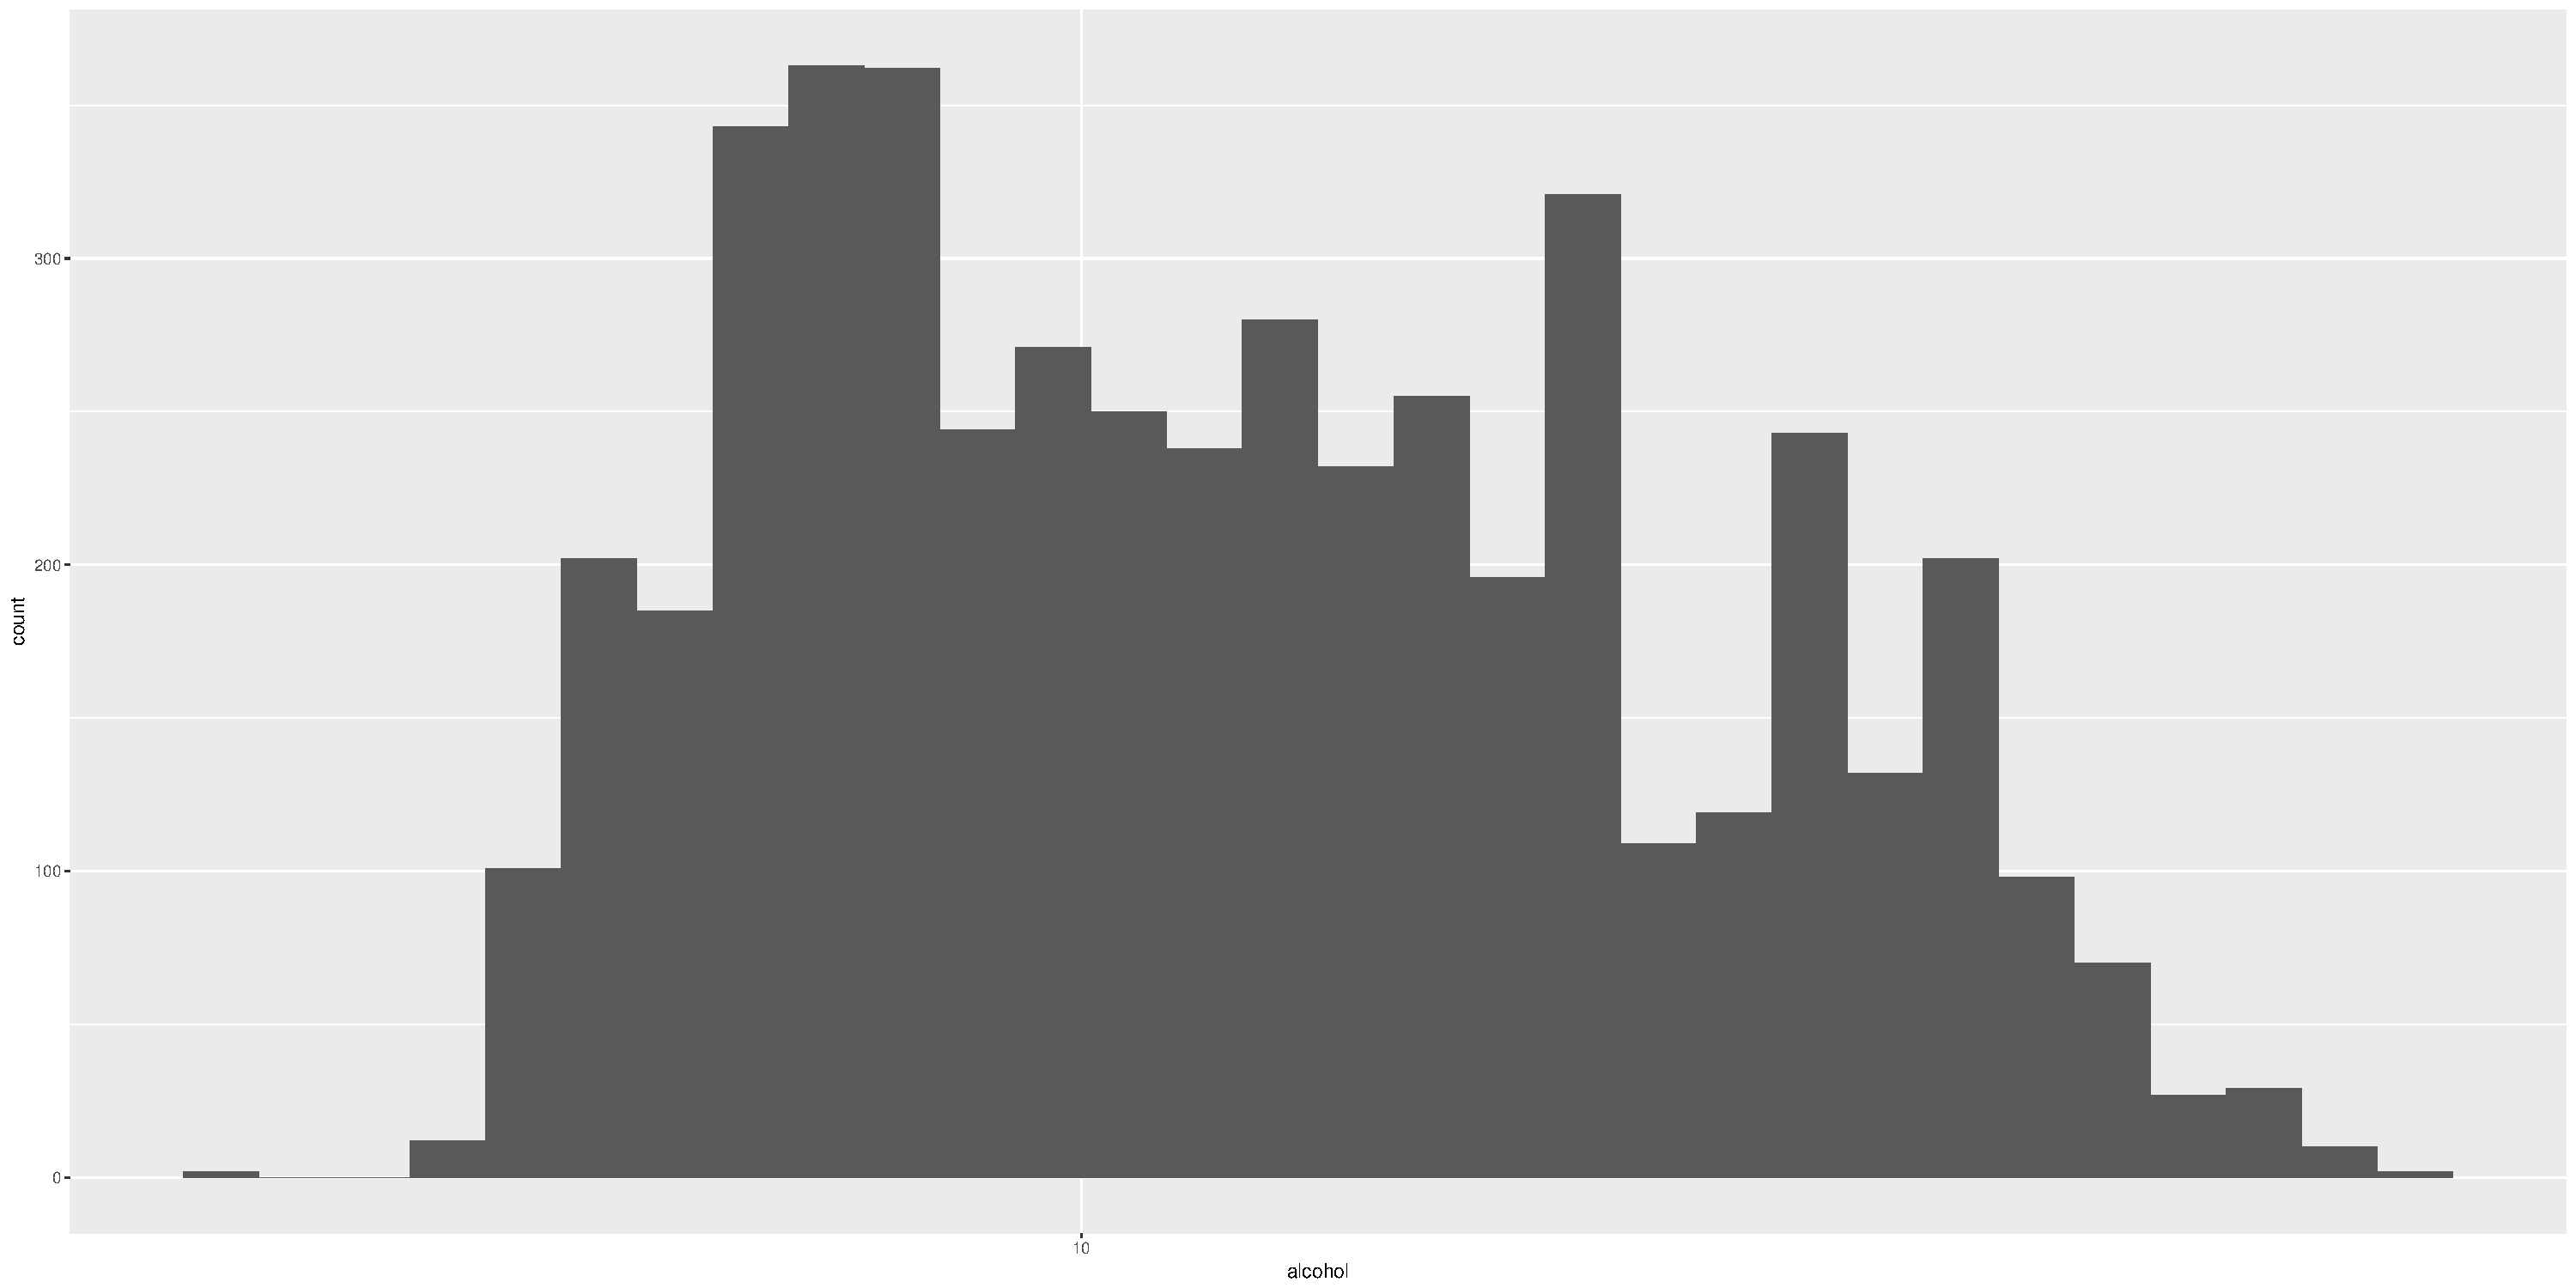
\includegraphics{White_wine_quality_files/figure-latex/unnamed-chunk-23-1.pdf}

From the quality rating histogram, we can see that the bulk of wines
have been rated 6, and only 5 wines have received a quality rating of 9,
which is the best

The histogram consists of discrete bars at 3,4,5,6,7,8 and 9.

\section{Univariate Analysis}\label{univariate-analysis}

\subsubsection{What is the structure of your
dataset?}\label{what-is-the-structure-of-your-dataset}

The dataset contains 4898 rows/observations with 13 variables/columns
eleven of the columns represent physicochemical properties of wines and
hold numerical values, one of the columns is the index/ID of each row
which is an integer and one of the columns holds the quality rating for
the wine which is also an integer

\subsubsection{What is/are the main feature(s) of interest in your
dataset?}\label{what-isare-the-main-features-of-interest-in-your-dataset}

The goal of this project is to investigate the influence of the
physicochemical properties on the quality of wine. Therefore, quality
rating is one of the main features of interest along with some other
properties.

\subsubsection{What other features in the dataset do you think will help
support your investigation into your feature(s) of
interest?}\label{what-other-features-in-the-dataset-do-you-think-will-help-support-your-investigation-into-your-features-of-interest}

Since quality rating is from sensory data, residual sugar and pH could
affect the sweetness/taste of wine and alcohol content could affect the
experience of wine consumption. But the investigation will look at all
the properties in the dataset

\subsubsection{Did you create any new variables from existing variables
in the
dataset?}\label{did-you-create-any-new-variables-from-existing-variables-in-the-dataset}

No, from just univariate exploration, it could not be ascertained if new
variables need to be created.It will be looked at if further exploration
gives rise to the need for creating more variables

\subsubsection{Of the features you investigated, were there any unusual
distributions?}\label{of-the-features-you-investigated-were-there-any-unusual-distributions}

\subsubsection{Did you perform any operations on the data to tidy,
adjust, or change the
form}\label{did-you-perform-any-operations-on-the-data-to-tidy-adjust-or-change-the-form}

\subsubsection{of the data? If so, why did you do
this?}\label{of-the-data-if-so-why-did-you-do-this}

The data was assessed for missing or duplicate values. It appeared
fairly tidy and prepared for analysis. Some distributions were heavily
skewed, so I used log transformation of data and tried trimming a
portion of the data to look at the distribution

\section{Bivariate Plots Section}\label{bivariate-plots-section}

Let us look at a scatterplot matrix to explore relationships between
variables. Let us leave `X' (which is the index/count) out. ```

\includegraphics{White_wine_quality_files/figure-latex/Bivariate_Plots-1.pdf}

We get a fair idea of the relationships from the scatterplot matrix but
it would be useful to go into the Pearson correlation coefficients for
the variables excluding quality It does not make sense to include the
`X' variable which is the index, when we want to look at correlations.
Since quality is a categorical ordinal variable, the Spearman
correlation coefficient should be calculated. So I am using the
dataframe excluding X and quality to look at Pearson coefficients

Let us generate a correlation matrix to get a visual idea about the
strength of the relationships

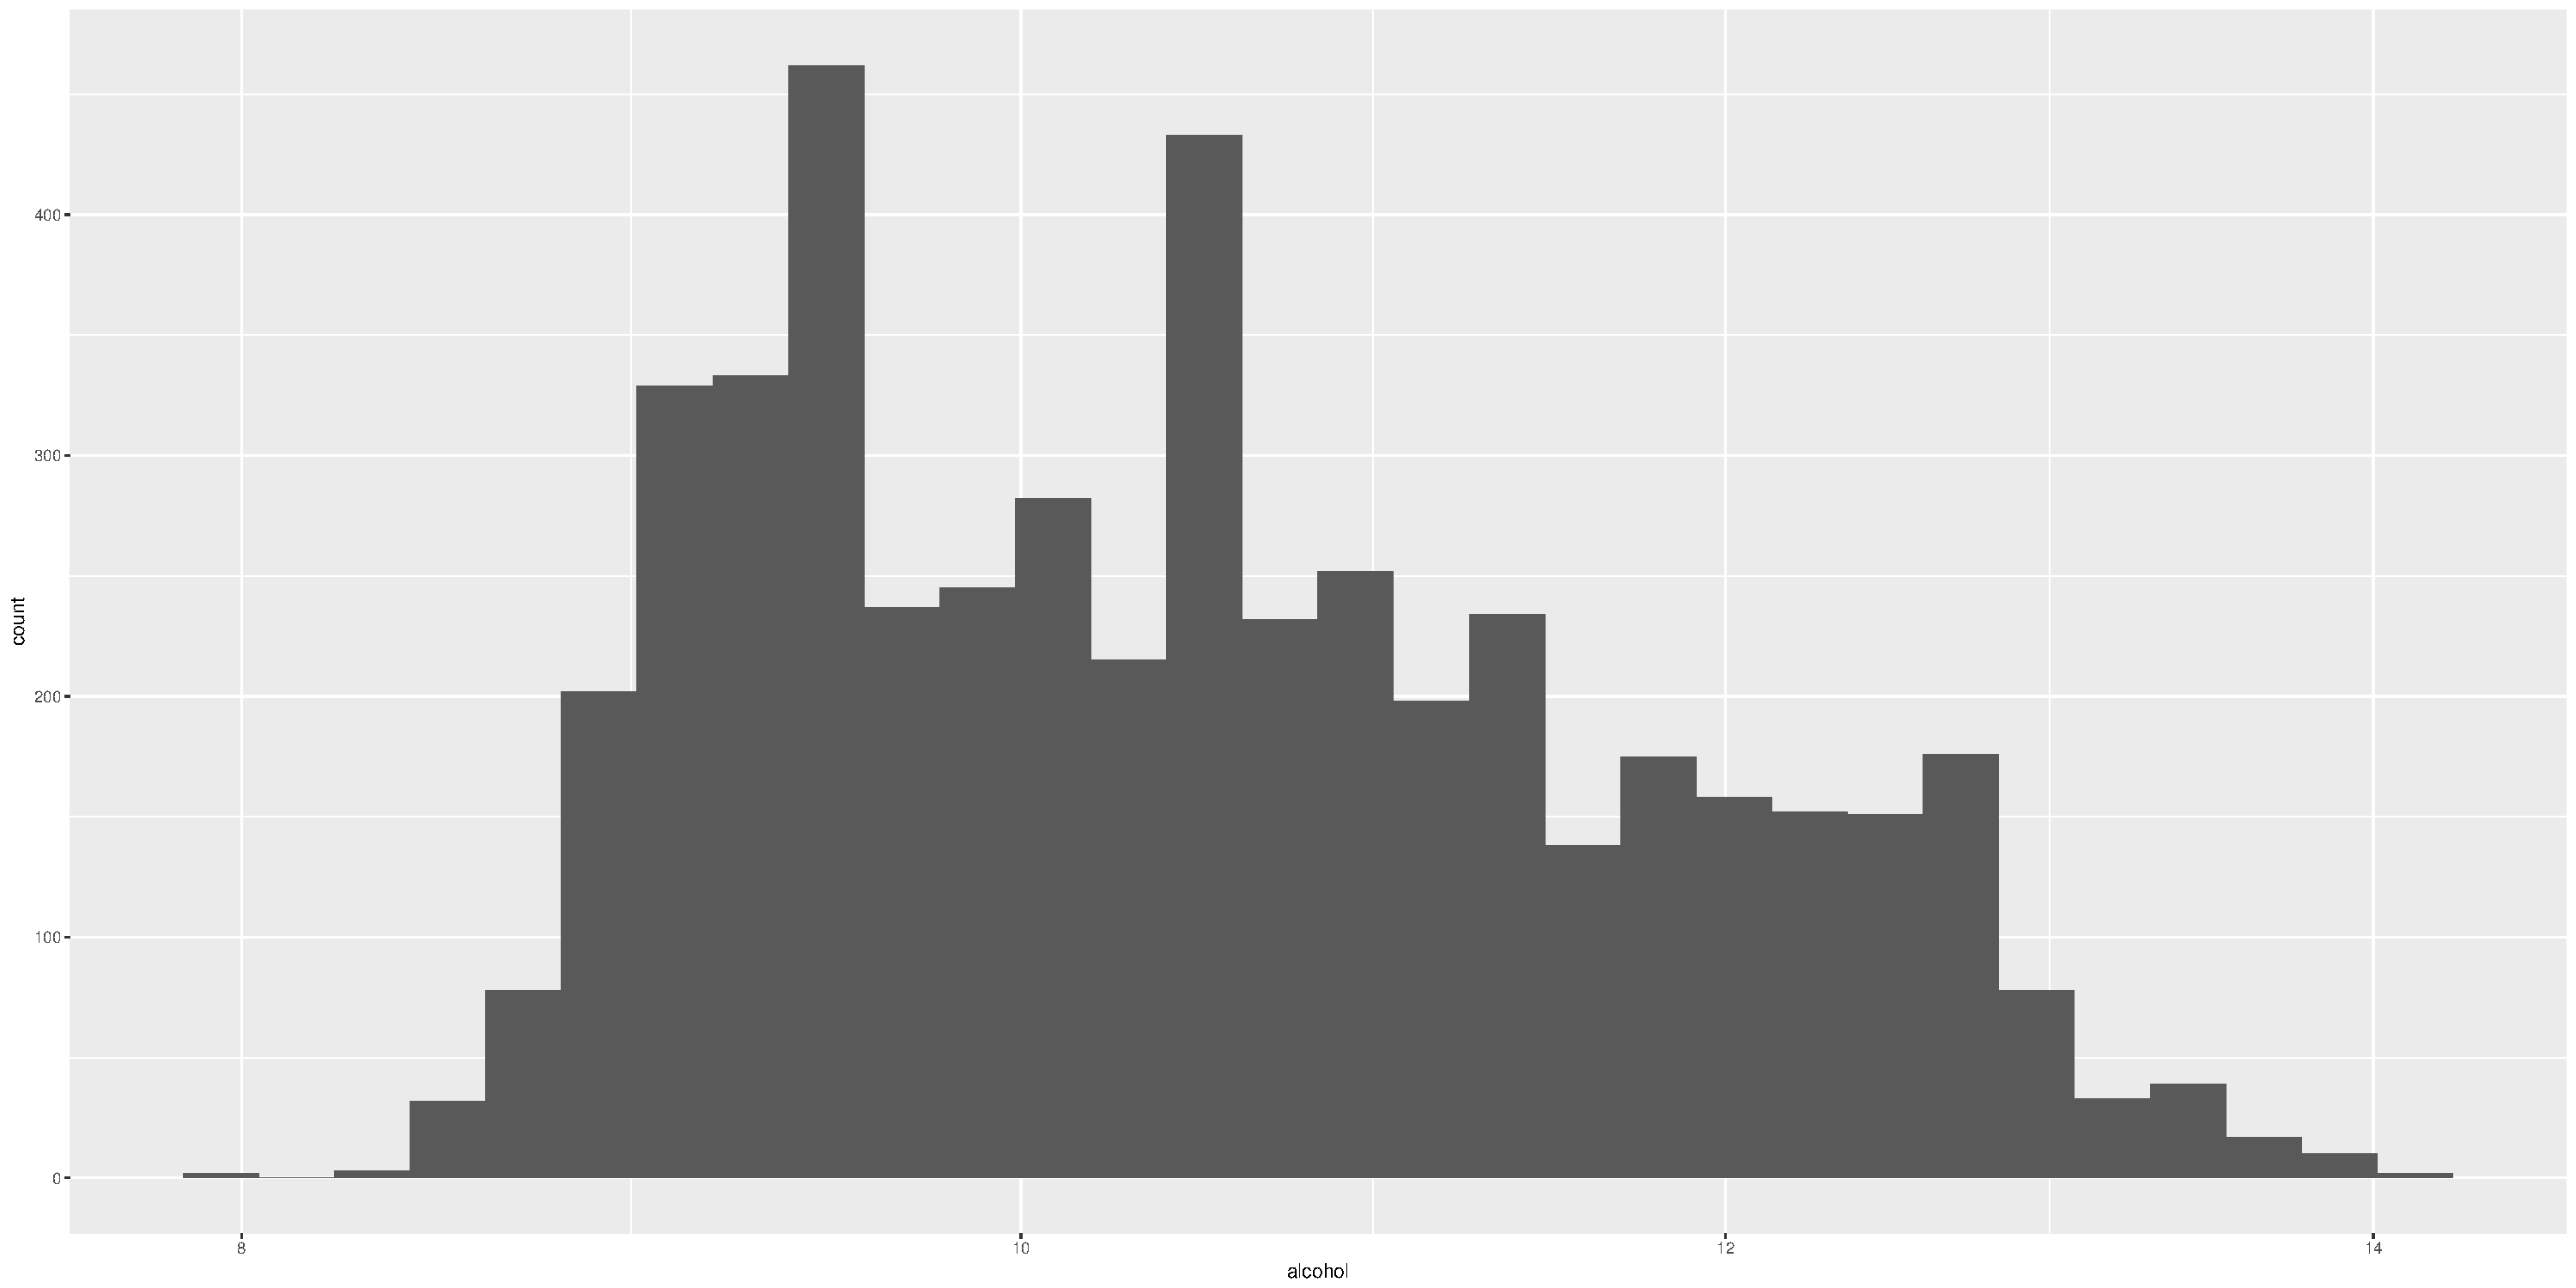
\includegraphics{White_wine_quality_files/figure-latex/unnamed-chunk-24-1.pdf}

Let's look closely at the correlation coefficicents from the above
visual

The values that are greater than \textbar{}0.3\textbar{} are interpreted
to be more meaningful as they signify a moderate/strong relationship

We see some moderate and some strong relationships from the visual
above:

\begin{itemize}
\item
  Fixed acidity and pH have a moderate negative correlation, which can
  be reasoned out as pH value decreases with increasing acidity
\item
  Residual sugar has a strong positive correlation with density which
  makes sense as more sugar makes the wine denser
\item
  Free and total sulphur dioxide have a strong positive relationship
  which is expected, because total sulphur dioxide is the sum of free
  and bound sulphurdioxide
\item
  Alcohol and density have a strong negative relationship suggesting
  that higher alcohol content results in lesser wine density . Alcohol
  is less dense than water, so this relationship seems to make sense
\end{itemize}

Let's plot the moderate correlations

Fixed acidity vs pH
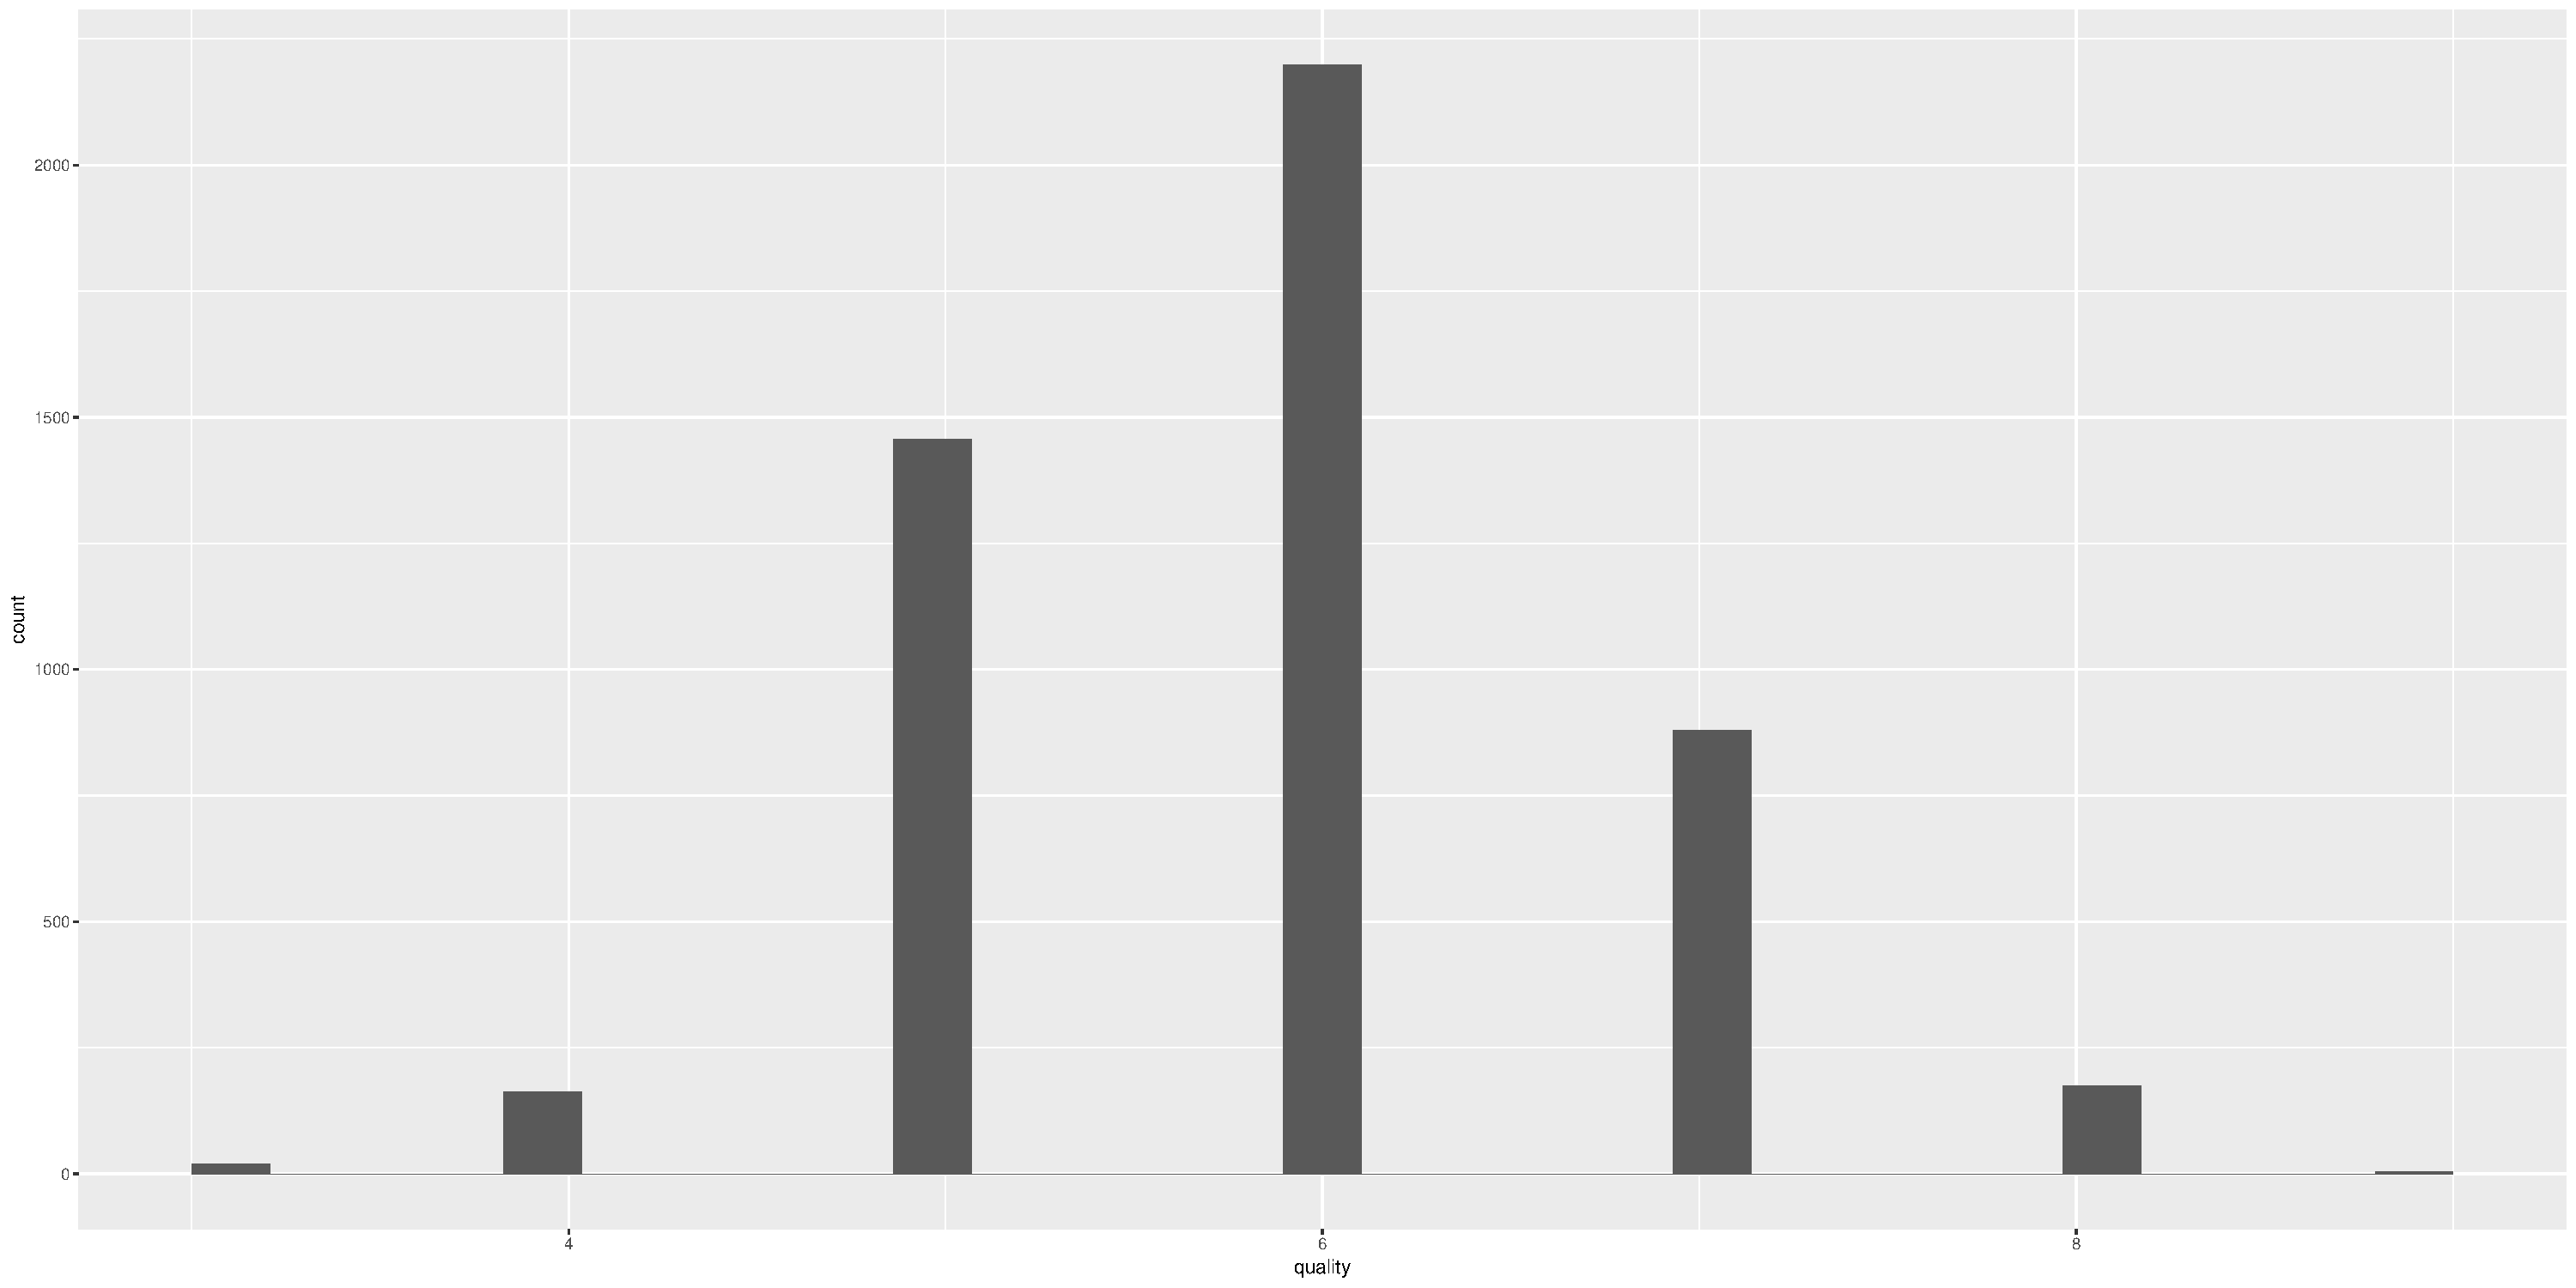
\includegraphics{White_wine_quality_files/figure-latex/unnamed-chunk-25-1.pdf}

Free Sulphur dioxide vs Total sulphur dioxide

\begin{verbatim}
## Warning: Removed 1 rows containing non-finite values (stat_smooth).
\end{verbatim}

\begin{verbatim}
## Warning: Removed 1 rows containing missing values (geom_point).
\end{verbatim}

\includegraphics{White_wine_quality_files/figure-latex/unnamed-chunk-26-1.pdf}

Let us visualize the strong relationships:

Residual sugar vs density

\includegraphics{White_wine_quality_files/figure-latex/unnamed-chunk-27-1.pdf}

Let's limit the axis to exclude outliers, reduce overplotting and look
at the plot with a linear trendline

\begin{verbatim}
## Warning: Removed 1 rows containing non-finite values (stat_smooth).
\end{verbatim}

\begin{verbatim}
## Warning: Removed 1 rows containing missing values (geom_point).
\end{verbatim}

\begin{verbatim}
## Warning: Removed 9 rows containing missing values (geom_smooth).
\end{verbatim}

\includegraphics{White_wine_quality_files/figure-latex/unnamed-chunk-28-1.pdf}

Let us visualize the relationship between alcohol and density

\includegraphics{White_wine_quality_files/figure-latex/unnamed-chunk-29-1.pdf}

Let's reduce overplotting and look at the plot again with a linear
trendline, excluding two outliers
\includegraphics{White_wine_quality_files/figure-latex/unnamed-chunk-30-1.pdf}

\subsubsection{Spearman's correlation coefficients for quality with
other
variables}\label{spearmans-correlation-coefficients-for-quality-with-other-variables}

Spearman's correlation is generally used when ordinal variables are
invloved. In this case we want to correlate continuous variables with an
ordinal variable. For the purpose of this course, I have used Spearman's
coefficient but there could be more complex but more suited methods to
accomplish this. The following are the Spearman correlation coefficients
for all variables with quality:

\begin{verbatim}
##        fixed.acidity     volatile.acidity          citric.acid 
##          -0.08448545          -0.19656168           0.01833273 
##       residual.sugar            chlorides  free.sulfur.dioxide 
##          -0.08206979          -0.31448848           0.02371338 
## total.sulfur.dioxide              density                   pH 
##          -0.19668029          -0.34835102           0.10936208 
##            sulphates              alcohol              quality 
##           0.03331897           0.44036918           1.00000000
\end{verbatim}

From the above values we find that - Quality and Chlorides are
moderately negatively correlated - Quality and density are moderately
negatively correlated - Quality and alcohol are positively correlated

\subsubsection{Creating some variables}\label{creating-some-variables}

\paragraph{Discrete Quality Variable}\label{discrete-quality-variable}

It would be helpful to create a discrete quality variable and view the
summary

\begin{verbatim}
##    3    4    5    6    7    8    9 
##   20  163 1457 2198  880  175    5
\end{verbatim}

\paragraph{Quality Bucket Variable}\label{quality-bucket-variable}

Let's also create a quality bucket variable

Summary of quality variable

\begin{verbatim}
##    Min. 1st Qu.  Median    Mean 3rd Qu.    Max. 
##   3.000   5.000   6.000   5.878   6.000   9.000
\end{verbatim}

Summary of quality buckets:

\begin{verbatim}
##      low moderate     high 
##      183     4535      180
\end{verbatim}

\paragraph{Residual Sugar bucket
variable}\label{residual-sugar-bucket-variable}

Summary statistics for residual sugar

\begin{verbatim}
##    Min. 1st Qu.  Median    Mean 3rd Qu.    Max. 
##   0.600   1.700   5.200   6.391   9.900  65.800
\end{verbatim}

Let's create a residual.sugar.bucket variable and view the summary

\begin{verbatim}
##    Low Medium   High 
##   1500   1604   1794
\end{verbatim}

\paragraph{Alcohol Bucket Variable}\label{alcohol-bucket-variable}

Let's create an alcohol.bucket variable

Summary Statistics for the alcohol bucket variable:

\begin{verbatim}
##      low moderate     high 
##     1436     2751      711
\end{verbatim}

\paragraph{Density Bucket Variable}\label{density-bucket-variable}

Summary of density

\begin{verbatim}
##    Min. 1st Qu.  Median    Mean 3rd Qu.    Max. 
##  0.9871  0.9917  0.9937  0.9940  0.9961  1.0390
\end{verbatim}

Let's create a density.bucket variable

Summary Statistics for the alcohol bucket variable:

\begin{verbatim}
##    low medium   high 
##   1446   1939   1513
\end{verbatim}

\subsubsection{Quality vs Chloride}\label{quality-vs-chloride}

Let's plot discrete quality ratings and chloride values to visualize the
relationship

\includegraphics{White_wine_quality_files/figure-latex/unnamed-chunk-43-1.pdf}

The relationship is not too clear from the box plot. However, the mean
Chloride values for the high quality wines are slightly lesser than the
lower quality wines

\paragraph{Quality vs Density}\label{quality-vs-density}

Let's look at the boxplot of density vs quality, excluding some density
outliers
\includegraphics{White_wine_quality_files/figure-latex/unnamed-chunk-44-1.pdf}

Summary statistics for wine density

\begin{verbatim}
##    Min. 1st Qu.  Median    Mean 3rd Qu.    Max. 
##  0.9871  0.9917  0.9937  0.9940  0.9961  1.0390
\end{verbatim}

Results for density statistics by quality level:

\begin{verbatim}
## quality: 3
##    Min. 1st Qu.  Median    Mean 3rd Qu.    Max. 
##  0.9911  0.9925  0.9944  0.9949  0.9969  1.0001 
## -------------------------------------------------------- 
## quality: 4
##    Min. 1st Qu.  Median    Mean 3rd Qu.    Max. 
##  0.9892  0.9926  0.9941  0.9943  0.9958  1.0004 
## -------------------------------------------------------- 
## quality: 5
##    Min. 1st Qu.  Median    Mean 3rd Qu.    Max. 
##  0.9872  0.9933  0.9953  0.9953  0.9972  1.0024 
## -------------------------------------------------------- 
## quality: 6
##    Min. 1st Qu.  Median    Mean 3rd Qu.    Max. 
##  0.9876  0.9917  0.9937  0.9940  0.9959  1.0390 
## -------------------------------------------------------- 
## quality: 7
##    Min. 1st Qu.  Median    Mean 3rd Qu.    Max. 
##  0.9871  0.9906  0.9918  0.9925  0.9937  1.0004 
## -------------------------------------------------------- 
## quality: 8
##    Min. 1st Qu.  Median    Mean 3rd Qu.    Max. 
##  0.9871  0.9903  0.9916  0.9922  0.9935  1.0006 
## -------------------------------------------------------- 
## quality: 9
##    Min. 1st Qu.  Median    Mean 3rd Qu.    Max. 
##  0.9897  0.9898  0.9903  0.9915  0.9906  0.9970
\end{verbatim}

Summary statistics for density by quality.bucket:

\begin{verbatim}
## quality.bucket: low
##    Min. 1st Qu.  Median    Mean 3rd Qu.    Max. 
##  0.9892  0.9926  0.9941  0.9943  0.9960  1.0004 
## -------------------------------------------------------- 
## quality.bucket: moderate
##    Min. 1st Qu.  Median    Mean 3rd Qu.    Max. 
##  0.9871  0.9918  0.9938  0.9941  0.9962  1.0390 
## -------------------------------------------------------- 
## quality.bucket: high
##    Min. 1st Qu.  Median    Mean 3rd Qu.    Max. 
##  0.9871  0.9903  0.9916  0.9922  0.9935  1.0006
\end{verbatim}

Summary statistics for density bucket by quality bucket:

\begin{verbatim}
## quality.bucket: low
##    low medium   high 
##     35     94     54 
## -------------------------------------------------------- 
## quality.bucket: moderate
##    low medium   high 
##   1305   1792   1438 
## -------------------------------------------------------- 
## quality.bucket: high
##    low medium   high 
##    106     53     21
\end{verbatim}

About 90\% of high quality wines fall in the low and medium density
buckets (60\% - low density and 30\% - medium density bucket) Only about
10\% of high quality wines have high density. In general, we see that
the mean density for high quality wines is lesser than that of low
quality wines

\paragraph{Quality vs Alcohol}\label{quality-vs-alcohol}

Let's look at the boxplot of alcohol vs quality
\includegraphics{White_wine_quality_files/figure-latex/unnamed-chunk-49-1.pdf}

It's interesting to see a clear trend of increasing alcohol content as
the quality of wine gets better.

Summary Statistics for Alcohol bucket variable

\begin{verbatim}
##    Min. 1st Qu.  Median    Mean 3rd Qu.    Max. 
##    8.00    9.50   10.40   10.51   11.40   14.20
\end{verbatim}

\begin{verbatim}
##      low moderate     high 
##      183     4535      180
\end{verbatim}

\begin{verbatim}
##    Mode   FALSE    TRUE 
## logical      34     146
\end{verbatim}

More than 80\% of high quality wines have alcohol content greater than
the mean alcohol content in wines

Summary Statistics for Alcohol bucket by Quality bucket

\begin{verbatim}
## quality.bucket: low
##      low moderate     high 
##       61      112       10 
## -------------------------------------------------------- 
## quality.bucket: moderate
##      low moderate     high 
##     1357     2564      614 
## -------------------------------------------------------- 
## quality.bucket: high
##      low moderate     high 
##       18       75       87
\end{verbatim}

Only 5\% of low quality wines have high alcohol content, while about
50\% of high quality wines have high alcohol content

\section{Bivariate Analysis}\label{bivariate-analysis}

\subsubsection{\texorpdfstring{Talk about some of the relationships you
observed in this part of the\\
investigation. How did the feature(s) of interest vary with other
features in\\
the
dataset?}{Talk about some of the relationships you observed in this part of the investigation. How did the feature(s) of interest vary with other features in the dataset?}}\label{talk-about-some-of-the-relationships-you-observed-in-this-part-of-the-investigation.-how-did-the-features-of-interest-vary-with-other-features-in-the-dataset}

From the bivariate exploration, it was seen that quality, which is the
main feature of interest did not strongly correlate with any of the
variables. Alcohol level, density and chlorides seemed to correlate
moderately with quality.

\subsubsection{\texorpdfstring{Did you observe any interesting
relationships between the other features\\
(not the main feature(s) of
interest)?}{Did you observe any interesting relationships between the other features (not the main feature(s) of interest)?}}\label{did-you-observe-any-interesting-relationships-between-the-other-features-not-the-main-features-of-interest}

Though quality did not directly correlate strongly with the variables,
alcohol level vs density and residual sugar vs density are strong
relationships. Fixed acidity acidity correlated negatively with pH which
makes sense from knowledge of general chemistry

High quality wines seem to have high alcohol content and low density

\subsubsection{What was the strongest relationship you
found?}\label{what-was-the-strongest-relationship-you-found}

\begin{itemize}
\tightlist
\item
  Density vs residual sugar (0.8)
\item
  Density vs alcohol (-0.8)
\end{itemize}

\section{Multivariate Plots Section}\label{multivariate-plots-section}

Let's pick the strongest relationships we saw in bivariate analysis and
add a third variable to the plots

I'm curious about residual sugar since it is a parameter that can affect
taste distinctly. So in the plot of density vs residual sugar, let us
see how adding information on the quality bucket helps us understand the
relationship The outliers for density have been excluded

\paragraph{Density vs residual sugar, by quality
bucket}\label{density-vs-residual-sugar-by-quality-bucket}

\includegraphics{White_wine_quality_files/figure-latex/Multivariate_Plots-1.pdf}

The gradient in color denoting quality is not very clear. There is
overplotting and the moderate quality wines are dominant

Let us subset the data to look at only low and high quality wines to see
if we can get clearer insight

\includegraphics{White_wine_quality_files/figure-latex/unnamed-chunk-54-1.pdf}
For a fixed value of density, the higher quality wines have more
residual sugar than the lower quality wines which is interesting.

Now let us color the density vs residual sugar plot by alcohol bucket

\includegraphics{White_wine_quality_files/figure-latex/unnamed-chunk-55-1.pdf}
Here the gradient in color denoting alcohol bucket looks very
interesting For a fixed density, wines with higher residual sugar have
greater alcohol content At higher levels of residual sugar, the density
is higher and alcohol content is lower

Let us facet the density vs residual sugar plot colored by alcohol using
quality.discrete

\includegraphics{White_wine_quality_files/figure-latex/unnamed-chunk-56-1.pdf}
The plots with lower quality ratings are dominated by wines with lower
alcohol As the quality rating increases, wines have higher alcohol and
lower density

\paragraph{Density vs alcohol level, by quality
bucket}\label{density-vs-alcohol-level-by-quality-bucket}

Let us add quality bucket tto our density vs alcohol plot excluding
density outliers
\includegraphics{White_wine_quality_files/figure-latex/unnamed-chunk-57-1.pdf}

Again we see that the moderate quality wines are dominant Let us subset
the data to include only low and high quality wines

\includegraphics{White_wine_quality_files/figure-latex/unnamed-chunk-58-1.pdf}

This plot shows us that wines with higher quality have higher alcohol
content and lower density. At lower alcohol levels, the variation in
density is more

Let us color the density vs alcohol plot by residual sugar

\includegraphics{White_wine_quality_files/figure-latex/unnamed-chunk-59-1.pdf}

We can seethat wines with higher residual sugar have higher density for
the same alcohol content

Now let's facet this graph by quality

\includegraphics{White_wine_quality_files/figure-latex/unnamed-chunk-60-1.pdf}
The variation in density decreases as quality gets better. the plots
with medium quality ratings are dominated by wines with high residual
sugar

Since alcohol vs quality was the strongest relationship we saw among all
the relationships with quality, let's explore that by coloring it by
residual sugar

\includegraphics{White_wine_quality_files/figure-latex/unnamed-chunk-61-1.pdf}

The buckets of residual sugar seem to be distributed among the levels of
quality, with a slight domination on the higher side of quality. Not
much can be ascertained about the influence of residual sugar on
quality.

As quality increases the alcohol content increases and the variation in
alcohol content decreases

\paragraph{Quality Prediction Model}\label{quality-prediction-model}

Let's try to build a mdel to predict quality given the values for a few
properties. Since quality is not strongly correlated with any of the
features the accuracy of the model cannot be expected to be high

Let's try using alcohol as the first feature since the correlation with
alcohol was highest for quality, The other features I'm choosing are:
density, chlorides and residual sugar

\begin{Shaded}
\begin{Highlighting}[]
\NormalTok{m1 <-}\StringTok{ }\KeywordTok{lm}\NormalTok{(}\KeywordTok{I}\NormalTok{(quality)}\OperatorTok{~}\KeywordTok{I}\NormalTok{(alcohol), }\DataTypeTok{data=}\NormalTok{wq)}
\NormalTok{m2 <-}\StringTok{ }\KeywordTok{update}\NormalTok{(m1, }\OperatorTok{~}\StringTok{ }\NormalTok{. }\OperatorTok{+}\StringTok{ }\NormalTok{density)}
\NormalTok{m3 <-}\StringTok{ }\KeywordTok{update}\NormalTok{(m2, }\OperatorTok{~}\StringTok{ }\NormalTok{. }\OperatorTok{+}\StringTok{ }\NormalTok{chlorides)}
\NormalTok{m4 <-}\StringTok{ }\KeywordTok{update}\NormalTok{(m3, }\OperatorTok{~}\StringTok{ }\NormalTok{. }\OperatorTok{+}\StringTok{ }\NormalTok{residual.sugar)}

\KeywordTok{mtable}\NormalTok{(m1, m2, m3, m4)}
\end{Highlighting}
\end{Shaded}

\begin{verbatim}
## 
## Calls:
## m1: lm(formula = I(quality) ~ I(alcohol), data = wq)
## m2: lm(formula = I(quality) ~ I(alcohol) + density, data = wq)
## m3: lm(formula = I(quality) ~ I(alcohol) + density + chlorides, data = wq)
## m4: lm(formula = I(quality) ~ I(alcohol) + density + chlorides + 
##     residual.sugar, data = wq)
## 
## ==========================================================================
##                        m1            m2            m3            m4       
## --------------------------------------------------------------------------
##   (Intercept)         2.582***    -22.492***    -21.150***     87.563***  
##                      (0.098)       (6.165)       (6.162)      (12.392)    
##   I(alcohol)          0.313***      0.360***      0.343***      0.237***  
##                      (0.009)       (0.015)       (0.015)       (0.018)    
##   density                          24.728***     23.671***    -84.931***  
##                                    (6.079)       (6.074)      (12.340)    
##   chlorides                                      -2.382***     -1.776**   
##                                                  (0.558)       (0.555)    
##   residual.sugar                                                0.052***  
##                                                                (0.005)    
## --------------------------------------------------------------------------
##   R-squared           0.190         0.192         0.195         0.212     
##   adj. R-squared      0.190         0.192         0.195         0.211     
##   sigma               0.797         0.796         0.795         0.787     
##   F                1146.395       583.290       396.315       328.736     
##   p                   0.000         0.000         0.000         0.000     
##   Log-likelihood  -5839.391     -5831.127     -5822.011     -5771.696     
##   Deviance         3112.257      3101.773      3090.247      3027.406     
##   AIC             11684.782     11670.255     11654.021     11555.391     
##   BIC             11704.272     11696.241     11686.504     11594.371     
##   N                4898          4898          4898          4898         
## ==========================================================================
\end{verbatim}

The R square values are very poor which implies we will have to adopt a
better approach to building a predictive model for quality. Using more
relevant features and complex methods may help build a better predictive
model for quality

\section{Multivariate Analysis}\label{multivariate-analysis}

\subsubsection{\texorpdfstring{Talk about some of the relationships you
observed in this part of the\\
investigation. Were there features that strengthened each other in terms
of\\
looking at your feature(s) of
interest?}{Talk about some of the relationships you observed in this part of the investigation. Were there features that strengthened each other in terms of looking at your feature(s) of interest?}}\label{talk-about-some-of-the-relationships-you-observed-in-this-part-of-the-investigation.-were-there-features-that-strengthened-each-other-in-terms-of-looking-at-your-features-of-interest}

Quality was the main feature of interest. Density and alcohol levels
seemed to influence quality and the relationships were explored more in
detail by introducing bucket variables for alcohol, quality, density and
residual sugar. But since none of the relationships were strong enough
to build a predictive model for quality, the R squared values for the
linear model are poor

\subsubsection{Were there any interesting or surprising interactions
between
features?}\label{were-there-any-interesting-or-surprising-interactions-between-features}

It was interesting to observe the variation in density / alcohol levels
as the quality gets better. Faceting plots by quality and coloring them
with a feature helped to understand and explain some trends

\subsubsection{\texorpdfstring{OPTIONAL: Did you create any models with
your dataset? Discuss the\\
strengths and limitations of your
model.}{OPTIONAL: Did you create any models with your dataset? Discuss the strengths and limitations of your model.}}\label{optional-did-you-create-any-models-with-your-dataset-discuss-the-strengths-and-limitations-of-your-model.}

\subsection{I tried to create a linear predictive model for quality
using alcohol, density, chlorides and residual sugar. Since the strength
of relationships with quality was not great, the model does very poorly.
More data with relevant features and more complex methods may help to
build a better
model}\label{i-tried-to-create-a-linear-predictive-model-for-quality-using-alcohol-density-chlorides-and-residual-sugar.-since-the-strength-of-relationships-with-quality-was-not-great-the-model-does-very-poorly.-more-data-with-relevant-features-and-more-complex-methods-may-help-to-build-a-better-model}

\section{Final Plots and Summary}\label{final-plots-and-summary}

\subsubsection{Plot One}\label{plot-one}

\includegraphics{White_wine_quality_files/figure-latex/Plot_One-1.pdf}

\subsubsection{Description One}\label{description-one}

This plot clearly illustrates that higher quality wines have higher
alcohol content. The black dots denote the mean alcohol content for
every quality level. The increasing trend in alcohol content is very
pronounced from rating 5 - 9. The strongest correlation observed with
quality was that of alcohol content with a Spearman's coefficient of
0.44

\subsubsection{Plot Two}\label{plot-two}

\includegraphics{White_wine_quality_files/figure-latex/Plot_Two-1.pdf}

\subsubsection{Description Two}\label{description-two}

This graph is colored by quality bucket and shows only the low and high
quality wines It is interesting to see that higher alcohol content
corresponds to lesser density (alcohol is less denser than water). From
Plot one and two, we can infer that higher quality wines have higher
alcohol and lesser density

\subsubsection{Plot Three}\label{plot-three}

\includegraphics{White_wine_quality_files/figure-latex/Plot_Three-1.pdf}

\subsubsection{Description Three}\label{description-three}

The variance in density with decreasing alcohol content is accounted for
by the residual sugar levels in wine. Density, alcohol and residual
sugar were part of strong correlations and this plot summarizes their
relationship. When this plot was faceted by quality it could further
help in picturing the variation of these parameters with quality.

\begin{center}\rule{0.5\linewidth}{\linethickness}\end{center}

\section{Reflection}\label{reflection}

Univariate explorationhelped get an idea about the individual
distributions of data and it was interesting to apply transformations
and see their effect.\\
I had expected residual sugar to be a direct influencer of taste and
therefore quality since the quality rating is sensory data. It turned
out that residual sugar correlated with density strongly and explained
the variance in density over alcohol and quality levels.

The interesting part of the exploration was investigating the strong
relationships between density and residual sugar, density and alcohol
and connecting them to quality ratings using colored and faceted plots.

Thelinear predictive model for quality was built using alcohol, density,
chlorides and residual sugar. Since the strength of relationships with
quality is not great, the model does very poorly. More data with
relevant features and more complex methods may help to build a better
model

\section{Resources}\label{resources}

\url{https://www.rdocumentation.org/packages/GGally/versions/1.3.2/topics/ggpairs}

\url{https://www.rdocumentation.org/packages/memisc/versions/0.99.14.9/topics/mtable}

\url{https://s3.amazonaws.com/udacity-hosted-downloads/ud651/wineQualityInfo.txt}


\end{document}
